\documentclass[12pt,a4paper,twoside,openright]{book}

\usepackage[italian]{babel}
\usepackage{style/isi-lt}
\usepackage{amssymb}
\usepackage{hyperref}
\usepackage{url}
\usepackage{listings}
\usepackage{graphicx}
\usepackage[export]{adjustbox}

\definecolor{dkgreen}{rgb}{0,0.6,0}
\definecolor{gray}{rgb}{0.5,0.5,0.5}
\definecolor{mauve}{rgb}{0.58,0,0.82}

\lstset{
  frame=single,
  captionpos=b,
  language=Java,
  aboveskip=3mm,
  belowskip=3mm,
  showstringspaces=false,
  columns=flexible,
  basicstyle={\small\ttfamily},
  numbers=none,
  numberstyle=\tiny\color{gray},
  keywordstyle=\color{blue},
  commentstyle=\color{dkgreen},
  stringstyle=\color{mauve},
  breaklines=true,
  breakatwhitespace=true,
  tabsize=3
}

%--------------------------------------------------------------------
%---------------------- INFORMAZIONI SULLA TESI ---------------------
%--------------------------------------------------------------------

\universita{Alma Mater Studiorum -- Università di Bologna}
\campus{Campus di Cesena}
\dipartimento{Dipartimento di Informatica -- Scienza e Ingegneria}
\cdl{Corso di Laurea in Ingegneria e Scienze Informatiche}

\titolo{Studio e analisi dell'architettura di applicazioni di realtà mista in HoloLens 2:\\un caso di studio}
\materia{Sistemi Embedded e Internet of Things}

\laureando{Filippo Vissani}

\relatore[Prof.]{Alessandro Ricci}
\correlatorea[Dott. Ing.]{Angelo Croatti}

\annoaccademico{2020 -- 2021}

\dedica{“Reality is what you want it to be.”

M. Pell}

\makeindex

\begin{document}
\frontmatter 

\maketitle
\tableofcontents

\chapter{Introduzione}
\markboth{INTRODUZIONE}{INTRODUZIONE}
Negli ultimi anni realtà virtuale e realtà aumentata hanno iniziato a diffondersi sempre più rapidamente.
Ogni anno vengono introdotte tecnologie che garantiscono esperienze sempre migliori.
Una di queste tecnologie è HoloLens 2, un dispositivo concepito da Microsoft per permettere esperienze di realtà mista.

In questa tesi si vogliono presentare i risultati degli studi effettuati sullo sviluppo di applicazioni Mixed Reality per HoloLens 2.

La realtà mista viene prima di tutto descritta da un punto di vista teorico, ma vengono anche definite architettura e struttura delle applicazioni relative.
L'obiettivo è quello di fornire una visione completa della Mixed Reality, non solo da un punto di vista teorico, ma anche tecnico e pratico.

Nel primo capitolo, dopo l'introduzione di alcuni cenni storici, vengono presentati i principali aspetti della realtà mista, che viene anche comparata alla realtà virtuale e alla realtà aumentata.
Successivamente vengono descritte la caratteristiche che un'applicazione Mixed Reality ha.
Infine, vengono introdotti i dispositivi attualmente in commercio che supportano questa tecnologia e i framework di sviluppo relativi.

Il secondo capitolo introduce HoloLens 2 da un punto di vista tecnico, insieme all'architettura e allo sviluppo di applicazioni Mixed Reality per questo dispositivo.
In questo capitolo vengono evidenziate le potenzialità del dispositivo e viene anche fornito un primo esempio di applicazione.

Nel terzo capitolo vengono descritti alcuni ambiti in cui l'applicazione di HoloLens 2 può migliorare determinati aspetti, come la produttività, l'efficienza e la sicurezza.

Per mostrare in pratica alcune delle potenzialità della Mixed Reality descritte nei capitoli precedenti, nel quarto capitolo viene presentato il caso di studio, relativo all'ambito sanitario. Qui viene fornita una descrizione dettagliata del caso, corredata dall'analisi dei requisiti e da una proposta di progetto.
Infine, viene definito lo sviluppo del prototipo relativo al progetto, in modo da rendere il lettore cosciente di cosa può fare HoloLens 2 concretamente. 
	
\mainmatter

\pagestyle{fancy} 
\fancyhead[LE,RO]{\thepage}
\fancyfoot{}

\chapter{Introduzione alla Mixed Reality}

\section{Cenni Storici}\label{sec:Sezione1.1}
I concetti di realtà virtuale (VR) e realtà aumentata (AR) comparirono per la prima volta nel 1965, quando Ivan Sutherland (ricercatore dell’Università di Harvard) pubblicò un saggio \cite{theultimatedisplay} contenente la seguente citazione:
\begin{center}
\textit{“The ultimate display would, of course, be a room within which the computer can control the existence of matter. A chair displayed in such a room would be good enough to sit in. Handcuffs displayed in such a room would be confining, and a bullet displayed in such a room would be fatal. With appropriate programming such a display could literally be the Wonderland into which Alice walked.”} 
\end{center}

\begin{figure}[t]
    \centering
    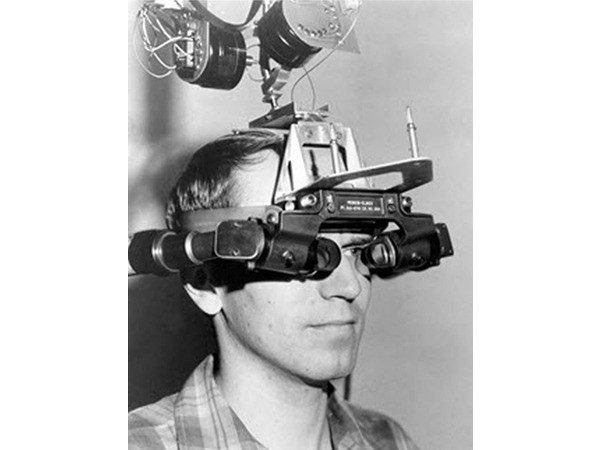
\includegraphics[width=\textwidth]{images/sword-of-damocles-vr.jpg}
    \caption{"La Spada di Damocle" è il soprannome dato al primo head mounted display al mondo, costruito da Ivan Sutherland nel 1968.}
    \label{fig:figure1}
\end{figure}

Anni dopo, nel 1968, Sutherland riuscì a sviluppare con successo il primo head-mounted display (HMD) della storia (Figura \ref{fig:figure1}). A causa del suo peso, doveva essere appeso al soffitto e per questo motivo venne soprannominato “Spada di Damocle”.

Lo sviluppo tecnologico avvenuto fra gli anni ‘80 e ‘90 fu fondamentale per permettere alla realtà aumentata di diventare un campo di ricerca indipendente. 

Il termine “realtà aumentata” venne coniato nel 1992 da Thomas Caudell e David Mizell \cite{Caudell}, impiegati alla Boeing Computer Services Research.
I due ricercatori svilupparono un HMD che permetteva di sovrapporre schemi specifici di un aereo (generati al computer) su schede riutilizzabili (Figura \ref{fig:figure12}). 
In questo modo, invece di riconfigurare manualmente ogni scheda per ogni fase del processo di produzione, le istruzioni di cablaggio personalizzate sarebbero state visualizzate dal lavoratore e modificate in modo rapido ed efficiente grazie al visore.

\begin{figure}[t]
    \centering
    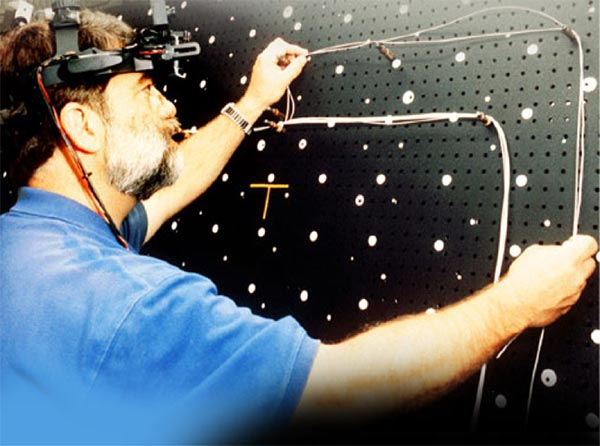
\includegraphics[width=\textwidth]{images/David-Mizell-AR.jpg}
    \caption{I ricercatori di Boeing hanno utilizzato un see-through HMD, creato da David Mizell, per guidare l'assemblaggio dei fasci di cavi per gli aerei.}
    \label{fig:figure12}
\end{figure}

Nel 1994 Paul Milgram pubblicò un articolo intitolato: “Augmented reality: A class of displays on the reality-virtuality continuum” \cite{Milgram}, introducendo i concetti di "reality-virtuality (RV) continuum" e di “mixed reality (MR)”, che definiscono la correlazione fra mondo reale e virtuale.

Negli anni successivi il campo della realtà aumentata ha continuato a evolversi e si è sempre più affermato nella cultura popolare. le tecnologie AR e VR sono diventate rapidamente di qualità superiore, più economiche e più ampiamente disponibili agli utenti.
\newpage
\section{Definizioni di VR, MR e AR}\label{sec:Sezione1.2}
Spesso i termini "realtà aumentata" e "realtà virtuale" vengono erroneamente interscambiati, quando in verità si tratta di due tecnologie con caratteristiche ben distinte.

Nella realtà aumentata le informazioni generate al computer vengono sovrapposte al mondo fisico, abbiamo quindi un mondo composto da una parte reale e una parte virtuale che sono in stretta correlazione fra loro. 

Entrando più nel dettaglio, gli aspetti chiave della realtà aumentata sono i seguenti:

\begin{itemize}
    \item Il mondo reale viene aumentato da informazioni digitali sovrapposte a esso.
    \item Le informazioni vengono visualizzate in registrazione spaziale e temporale con il mondo fisico.
    \item Le informazioni visualizzate dipendono dalla posizione e dalla prospettiva dell’utente nel mondo reale.
    \item L'esperienza di realtà aumentata è interattiva, ovvero l’utente può interagire con le informazioni e apportare modifiche a esse.
    \item Il livello d'interattività può variare dal semplice cambiamento della prospettiva alla manipolazione e persino alla creazione di nuove informazioni.
\end{itemize}

Nella realtà virtuale invece l’utente viene proiettato in un ambiente generato interamente al computer, non necessariamente correlato con il mondo reale.
I sensi vengono occlusi in tutto o in parte, in modo da far sembrare reale l’ambiente creato artificialmente.
Una volta definite le caratteristiche di queste due tecnologie la domanda che sorge spontanea è:
\begin{center}
"Che rapporto c’è fra VR e AR?"
\end{center}
La risposta la diede Paul Milgram nel 1994, pubblicando “Augmented Reality: A class of displays on the reality-virtuality continuum” \cite{Milgram} che, come detto nella sezione \ref{sec:Sezione1.1}, definisce i concetti di Reality-Virtuality Continuum e di Mixed Reality. 

Il RV continuum presenta una gamma di realtà che varia dal completamente reale al completamente virtuale (Figura \ref{fig:figure13}).
Secondo Milgram tutto ciò che risiede fra questi due estremi fa parte della Mixed Reality, che è composta dalla Augmented Reality, dove la realtà viene aumentata da entità virtuali e dalla Augmented Virtuality, dove il mondo virtuale viene aumentato da entità appartenenti al mondo reale.
\begin{figure}[t]
    \centering
    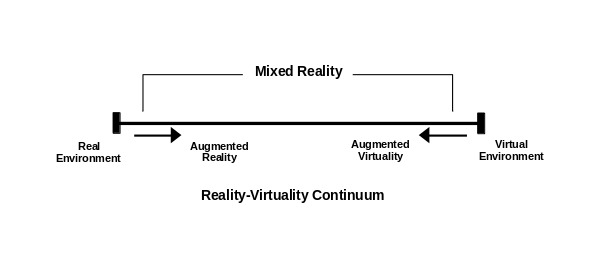
\includegraphics[width=\textwidth]{images/RV-continuum.jpg}
    \caption{Rappresentazione semplificata del Reality-Virtuality Continuum teorizzato da Paul Milgram.}
    \label{fig:figure13}
\end{figure}

Ciò che distingue la realtà mista da quella virtuale è l'integrazione delle entità virtuali nell'ambiente, chiamata registrazione spaziale; queste infatti, hanno una posizione e occupano uno spazio nel mondo fisico esattamente come se fossero reali, mentre nelle applicazioni AR il contenuto digitale si sovrappone al mondo reale senza integrarsi.
La Figura \ref{fig:figure14} descrive meglio questo concetto: abbiamo un’applicazione MR che introduce entità virtuali all’interno di un ambiente reale; 
la posizione di queste entità non dipende dalla posizione dell’utente nell’ambiente, quindi se ad esempio l’utente si spostasse verso un altro lato del tavolo vedrebbe la casa virtuale da un’altra prospettiva. 
Naturalmente è possibile anche interagire con le entità virtuali, che possono essere spostate, ridimensionate o anche eliminate.

\begin{figure}[t]
    \centering
    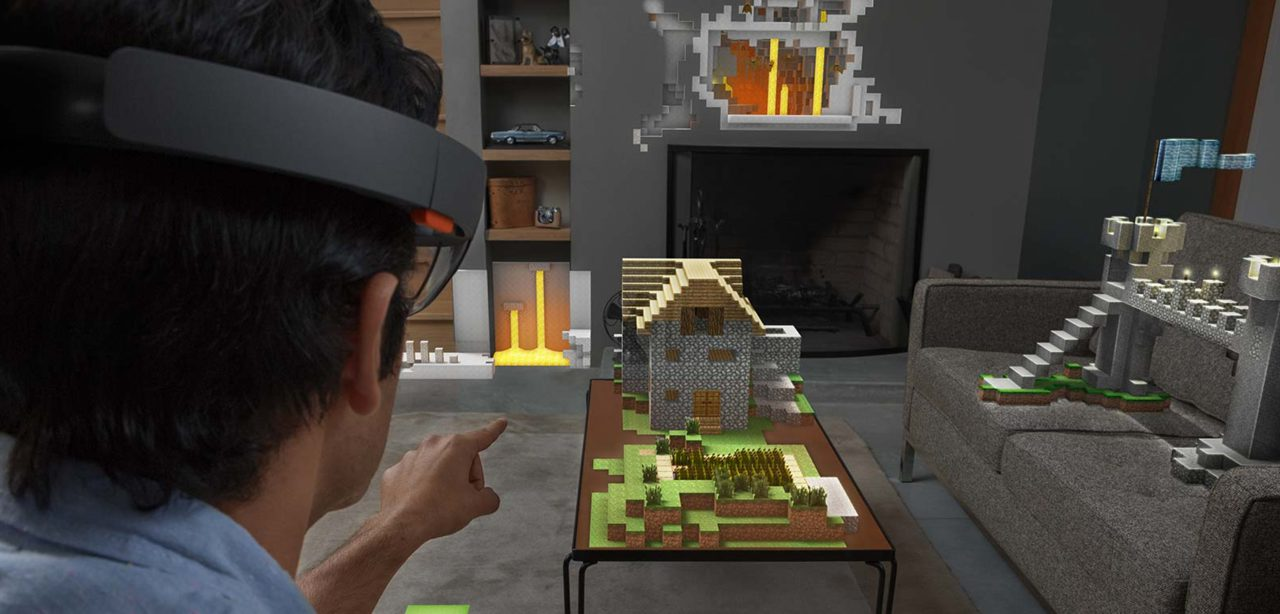
\includegraphics[width=\textwidth]{images/hololens-ar.jpg}
    \caption{Applicazione AR in cui le entità virtuali occupano una posizione nel mondo reale indipendentemente dalla collocazione e dai movimenti dell’utente.}
    \label{fig:figure14}
\end{figure}

In un certo senso, le entità digitali devono essere gestite come oggetti fisici almeno per quanto riguarda la questione della registrazione. Per questo motivo la registrazione con il mondo reale deve essere sia spaziale che temporale.

\section{Caratteristiche di un'Applicazione MR}\label{sec:Sezione1.3}
Nelle applicazioni MR le entità digitali vengono rappresentate dagli ologrammi (Figura \ref{fig:figure14}), che possono assumere qualsiasi forma ed emettere suoni. Inoltre, gli ologrammi possono modificare lo spazio fisico arricchendolo.

Ogni volta che un sistema software basato su AR deve aggiornare la vista dell'utente sull'ambiente Mixed Reality per mostrargli gli ologrammi, vengono richiesti due passaggi. Prima di tutto, il sistema deve identificare lo stato attuale del mondo fisico e calcolare di conseguenza lo stato del mondo digitale. In secondo luogo, emerge l'esigenza di visualizzare ologrammi in registrazione con la realtà in modo efficace considerando le percezioni umane. Generalmente lo stato in tempo reale del mondo fisico è ottenuto sfruttando i sensori forniti dal dispositivo, in particolare a questo scopo vengono utilizzate telecamere e tecniche di computer vision. Un problema significativo nella realtà aumentata è sapere dove si trova l'utente rispetto al sistema di riferimento del mondo reale, ovvero occuparsi del rilevamento del movimento e della posizione.

\subsection{Determinare la Posizione dell'Utente}
Nella realtà aumentata, determinare la prospettiva dell'utente significa calcolare la posa della telecamera, che è rappresentata da una posizione nello spazio 3D con sei gradi di libertà (6DOF). La posa si riferisce alla posizione e all'orientamento della fotocamera. Per identificare la posa della fotocamera è possibile utilizzare sensori inerziali (come accelerometro o giroscopio) e di posizione (come bussola o GPS). Una volta rilevata la posa della fotocamera, ovvero quando il sistema conosce la posizione e l'orientamento attuali dell'utente, gli ologrammi e i contenuti digitali possono essere presentati in allineamento con il mondo reale e proposti all'utente in un dato momento secondo la sua prospettiva. Secondo la letteratura, possono essere considerate diverse tecniche, eventualmente combinate, per determinare dove si trova l'utente e quale è il suo punto di vista. La tecnica più elementare, nota come AR marker based, dove il marker viene utilizzato per consentire il tracciamento al fine di determinare la posa del dispositivo. Oltre ai marker, possono essere applicate anche tecniche di tracciamento visivo in tempo reale. In particolare, il riferimento è a quelle tecniche che consentono una mappatura continua del mondo reale sfruttando un ampio insieme di punti rilevati, note anche come markerless AR.

Comunemente, un marker è un'immagine 2D asimmetrica che rappresenta un pattern molto semplice con l'obiettivo di essere rapidamente riconoscibile dagli algoritmi di visione artificiale (tipicamente modelli quadrati, in bianco e nero). In alcuni casi (ad esempio sfruttando Vuforia) è possibile sfruttare anche oggetti 3D come marker.
Grazie alla loro forma e struttura predefiniti, i marker possono essere localizzati facilmente dal visore. Quindi, vengono utilizzati per un rapido calcolo della posa.
Inoltre, per quanto riguarda quelli 2D, l'elevato contrasto dei quadrati in bianco e nero aiuta a facilitare il rilevamento.
I marker vengono posizionati nell'ambiente reale con lo scopo di individuare un sistema di riferimento da utilizzare per accoppiare il layer digitale con quello reale. Utilizzando un marker posto in una posizione ben nota del mondo reale, la funzione di tracciamento utilizza la fotocamera per stimare la posa del dispositivo in tempo reale in base a ciò che sta "vedendo". 

In condizioni di scarsa illuminazione o quando la telecamera è lontana dal marker tracciato, è possibile utilizzare tecniche basate sul rilevamento di \textit{natural feature point}.
Natural Feature Tracking (NFT) è una tecnica AR per riconoscere e tracciare una scena per determinare la posa della fotocamera, evitando deliberatamente di usare i marker.
NFT può sfruttare elementi incorporati nel mondo reale per migliorare i punti e le regioni di tracciamento. Il risultato può essere definito "markerless tracking" perché i "marker" non sono visibili all'utente.
Sebbene gli approcci senza marker possano sembrare la soluzione migliore, bisogna tenere in considerazione che tracciare la posa della fotocamera in ambienti sconosciuti può essere complicato. Negli ultimi anni è stata sviluppata una tecnologia nota come SLAM (Simultaneous Localization and Mapping), che ridefinisce l'idea originale di AR markerless basata su feature point. Tuttavia, l'NFT può essere meno costoso dal punto di vista computazionale di un sistema SLAM completo e generalmente è più adatto per i dispositivi mobili.
SLAM inizia con un ambiente sconosciuto e vuoto in cui il dispositivo di realtà aumentata cerca di generare una mappa e localizzarsi all'interno di essa. Attraverso una serie di algoritmi computazionalmente costosi, SLAM utilizza i dati del sensore IMU (unità di misura inerziale) per costruire una mappa dell'ambiente sconosciuto e allo stesso tempo per identificare la sua posizione.
Infine, l'AR markerless utilizza in genere anche la funzione GPS per tracciare la posizione dell'utente in scenari all'aperto combinata con il tracciamento visivo per ottenere l'orientamento correlato. 

\subsection{Sistemi di Coordinate}
Per familiarità, accuratezza e semplicità, la maggior parte degli ambienti virtuali è definita utilizzando un sistema di coordinate cartesiane standard, come mostrato in Figura \ref{fig:figure15}. All'interno di questo sistema, ogni punto è specificato in modo univoco utilizzando tre coordinate numeriche (x, y, z) che rappresentano distanze specifiche (misurate nella stessa unità di lunghezza) da tre piani reciprocamente perpendicolari. 

Oltre a essere l'approccio più comunemente utilizzato per la mappatura di spazi reali e virtuali, il sistema cartesiano viene impiegato anche per definire la posizione e il punto di vista di un utente nello spazio.

\begin{figure}[H]
    \centering
    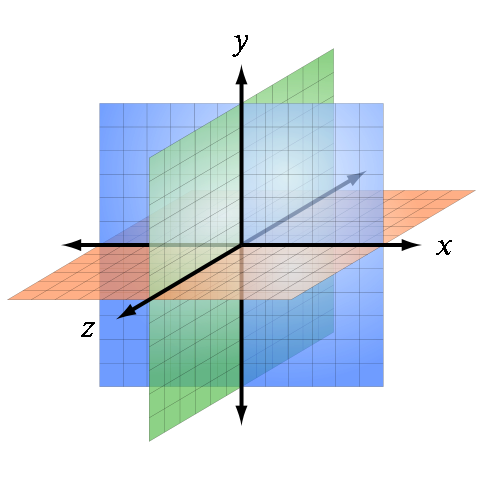
\includegraphics[width=0.6\textwidth]{images/sistema-cartesiano.png}
    \caption{Ogni punto nel sistema di coordinate cartesiane 3D è identificato in modo univoco da valori x, y e z.}
    \label{fig:figure15}
\end{figure}

Un ologramma posto in un ambiente tridimensionale deve avere l'abilità di muoversi liberamente e di ruotare sui tre assi perpendicolari.
Poiché il movimento lungo ognuno degli assi è indipendente quanto per gli assi di traslazione che per gli assi di rotazione, il movimento ha quindi sei gradi di libertà (6DoF: Six Degrees Of Freedom).
Per garantire questa caratteristica è possibile sfruttare gli angoli di Eulero o i quaternioni.
Solitamente vengono utilizzati i quaternioni perché con gli angoli di Eulero può presentarsi il fenomeno del blocco cardanico (in inglese gimbal lock), che avviene quando vengono allineati i due assi rotanti verso la stessa direzione, causando la perdita di un grado di libertà sull'asse bloccato.

\subsection{Interazioni con gli Ologrammi}
La realtà aumentata è, per sua natura, un mezzo interattivo. Se il contenuto digitale deve essere percepito come parte del mondo reale, poiché le persone possono interagire con oggetti fisici anche nei sistemi AR gli utenti dovrebbero essere in grado di interagire con gli ologrammi in modo simile. In effetti, l'interazione gioca un ruolo chiave nell'esperienza complessiva dell'utente. In un ambiente AR, l'interazione è generalmente limitata all'azione da eseguire sugli elementi digitali, ad esempio osservarli o afferrarli e spostarli da una posizione a un'altra. L'interazione in AR è un aspetto che dipende principalmente dal dispositivo utilizzato per tracciare e mostrare ologrammi nell'ambiente Mixed Reality. La capacità di interagire con gli ologrammi aumenta proporzionalmente e diventa più potente in relazione all'efficienza del dispositivo AR utilizzato in termini di propri sensori e capacità computazionali. 

\subsection{Esperienze Multi-Utente}
Il mondo reale è un ambiente cooperativo multiutente, gli ambienti di realtà mista diventano più interessanti quando anche il livello digitale e gli ologrammi possono essere condivisi tra più utenti che interagiscono contemporaneamente. Proporre un'esperienza multiutente cooperativa significa avere un layer digitale condiviso in tempo reale. Prima di tutto, gli utenti dovrebbero essere in grado di osservare gli stessi ologrammi ma dalla propria prospettiva. In questo caso, utilizzando dei marker, questa caratteristica potrebbe essere semplicemente ottenuta, ad esempio, con due utenti che osservano contemporaneamente lo stesso marker che propone per entrambi gli stessi sistemi di riferimento e orientamento. Sfortunatamente, questa è una soluzione che nasconde il vero problema: in questo caso, lo stato dell'ologramma non è realmente condiviso tra gli utenti. Ad esempio, se un utente sposta l'ologramma, l'altro utente continuerà a vedere l'ologramma nella posizione originale. Per risolvere i problemi proposti c'è l'esigenza che entrambi gli utenti facciano riferimento alla stessa istanza dell'ologramma osservato da entrambi, una sorta di centralizzazione dell'istanza del livello digitale, a cui accedono più utenti. Non sorprende che per sperimentare un ambiente MR multiutente cooperativo completo emergano esigenze che sono ben lungi dall'essere affrontate dalle soluzioni infrastrutturali software attualmente disponibili. Soprattutto quando la cooperazione non è intesa solo tra umani ma coinvolge anche entità software autonome e altre cose fisiche appartenenti al mondo reale.
Un altro problema è dato dai diversi dispositivi che si possono usare per accedere all'esperienza condivisa. Con dispositivi (ad esempio smartphone e visori) basati su piattaforme differenti (come Windows, Lumin OS, Android e iOS) sorge l'esigenza di sviluppare API comuni per garantire l'interoperabilità delle applicazioni MR indipendentemente dalla piattaforma che si sta utilizzando.
Una delle soluzioni proposte per venire a capo di questo problema è OpenXR, ovvero un'API che si occupa di fornire un accesso nativo alle piattaforme e ai dispositivi di
Augmented, Mixed e Virtual Reality.

\section{Tassonomia dei Dispositivi MR}\label{sec:Sezione1.4}
Al giorno d’oggi è disponibile una moltitudine di dispositivi MR, che si contraddistinguono in base ai sistemi di input, output ed elaborazione che utilizzano. 

In generale, è possibile identificare due macrocategorie di sistemi AR: wearable (indossabili) e non-wearable (non indossabili). 

Un’altra suddivisione può essere fatta distinguendo i dispositivi che sono stati concepiti appositamente per esperienze MR da quelli più generici (come PC e smartphone).

Alcuni dispositivi, come le lenti a contatto per la realtà aumentata, sono ancora in fase di sviluppo e non sono ancora disponibili prodotti commerciali.

\subsection{Head Mounted Display}
Un head mounted display è un visore incorporato in un casco, dotato di dispositivi di registrazione dell'orientamento per il movimento sincronizzato della testa e degli occhi dell’utente.
Esistono due tipi di HMD attualmente in commercio, quelli che supportano esclusivamente esperienze VR (HTC Vive e Oculus Rift, Figura \ref{fig:figure16}) e quelli progettati per esperienze AR (come HoloLens 2 e Magic Leap 1, Figura \ref{fig:figure17}).

\begin{figure}[H]
    \centering
    \begin{subfigure}[b]{0.4\textwidth}
        \centering
        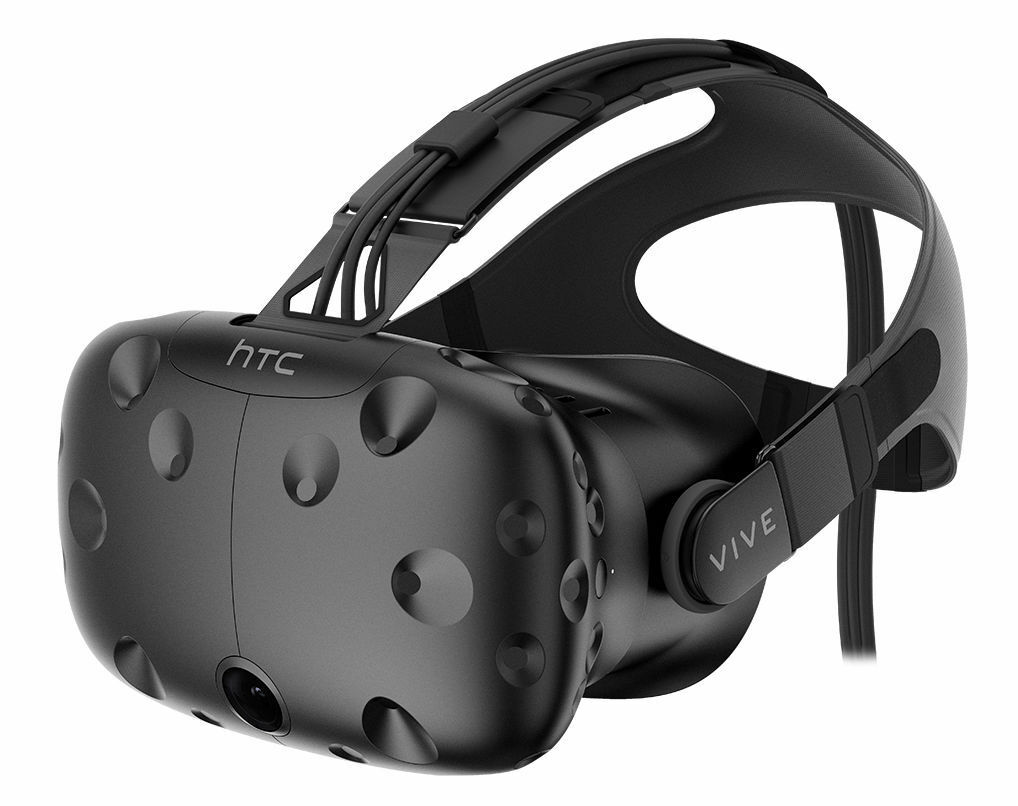
\includegraphics[width=\textwidth]{images/HTC-Vive.JPG}
        \caption{HTC Vive}
        \label{fig:figure16a}
    \end{subfigure}
    \begin{subfigure}[b]{0.4\textwidth}
        \centering
        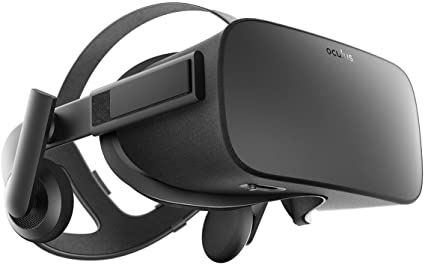
\includegraphics[width=\textwidth]{images/Oculus-Rift.jpg}
        \caption{Oculus Rift}
        \label{fig:figure16b}
    \end{subfigure}
       \caption{HTC Vive e Oculus Rift messi a confronto}
       \label{fig:figure16}
\end{figure}

Rift utilizza un singolo sensore esterno, un cilindro nero che si trova su un supporto da tavolo in metallo alto 23 centimetri. Il sensore può inclinarsi verso l'alto e verso il basso e deve essere posizionato in un punto in cui possa mantenere una visione chiara del visore quando è in uso. Un secondo sensore identico traccia i controller Oculus Touch, questi due sensori inoltre lavorano in tandem per migliorare il tracciamento di tutti i dispositivi e coprire un'area più ampia rispetto alla posizione fissa consentita da un solo sensore. 

HTC Vive è composto non solo da un visore per la realtà virtuale e da due sofisticati controller, ma anche da un sistema di due telecamere laser (base station) che hanno il compito di tracciare il movimento dell'utente all’interno della stanza. HTC Vive supporta un’area che può avere una dimensione massima di cinque metri di diagonale, pari alla massima distanza consigliata per le due base station, sufficiente per coprire interamente una stanza di circa 12 metri quadri, e dare così l’impressione di potersi muovere liberamente nel mondo virtuale.

Gli HMD che supportano la realtà aumentata sfruttano una tecnologia definita \textit{optical see-through}, che permette di vedere attraverso il display.

Magic Leap 1 è dotato di uno schermo LCOS prodotto da Omnivision, che offre una definizione di 1280 x 960. Mentre il primo HoloLens aveva uno schermo con definizione HD (720p) e un campo visivo di 30 gradi, il suo successore è stato migliorato notevolmente e infatti ha un campo visivo di 52 gradi. HoloLens 2 supera Magic Leap in termini di definizione con il suo schermo che offre una definizione di circa 2K per occhio. In totale, questo nuovo visore visualizza 47 pixel per grado. Lo schermo di HoloLens 2 è quindi superiore in termini di definizione, mentre i due visori AR sono uguali in termini di campo visivo.

\begin{figure}[t]
    \centering
    \begin{subfigure}[b]{0.4\textwidth}
        \centering
        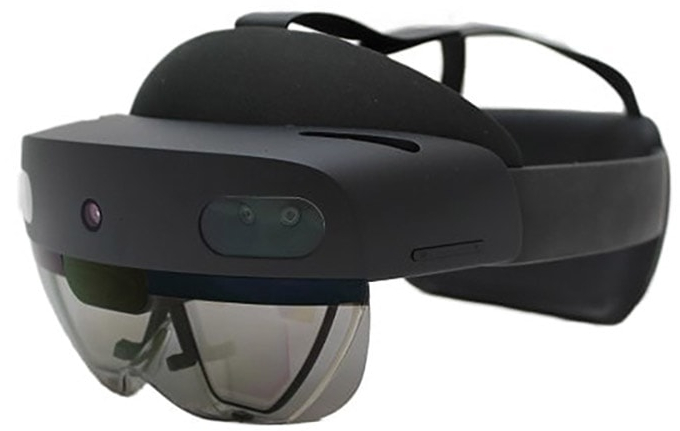
\includegraphics[width=\textwidth]{images/Hololens2.jpg}
        \caption{Microsoft HoloLens 2}
        \label{fig:figure17a}
    \end{subfigure}
    \begin{subfigure}[b]{0.55\textwidth}
        \centering
        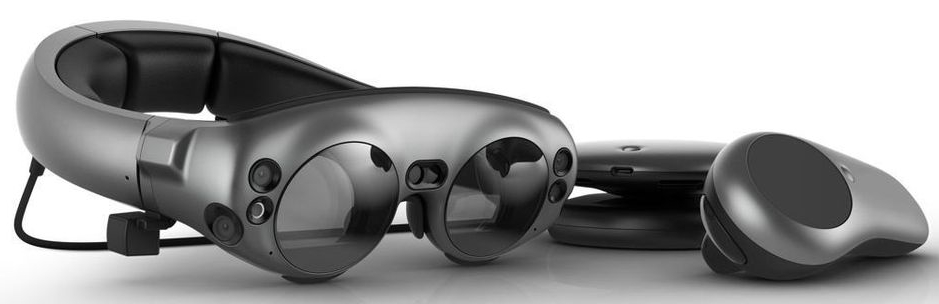
\includegraphics[width=\textwidth]{images/Magic-Leap1.jpg}
        \caption{Magic Leap 1}
        \label{fig:figure17b}
    \end{subfigure}
       \caption{HoloLens 2 e Magic Leap 1 messi a confronto}
       \label{fig:figure17}
\end{figure}

Magic Leap 1 viene fornito con il suo controller "Control". Questo controller offre sei gradi di libertà di movimento senza la necessità di sensori esterni aggiuntivi. Si basa sul tracciamento del campo elettromagnetico. È questo accessorio, simile ai controller per visori VR Oculus Rift o HTC Vive, che permette di interagire nella realtà aumentata di Magic Leap.
Magic Leap 1 offre anche funzioni di tracciamento dell'iride e della mano. Quest'ultimo punto permette di interagire usando le mani in modo naturale. In realtà, questo sistema non rileva la posizione delle dita dell'utente nello spazio, ma solo gesture predefinite.
HoloLens 2 si distingue per una tecnologia di tracciamento della mano decisamente accurata. Infatti, questo nuovo visore AR è in grado di seguire la posizione delle dieci dita dell'utente. Pertanto, è persino possibile suonare il pianoforte in realtà aumentata.
Come con il primo HoloLens, purtroppo, è ancora necessario che le mani rimangano nel campo visivo di HoloLens 2 per il tracciamento.
Troviamo anche la stessa tecnologia di eye tracking degli smartphone Lumia. L'Eye Tracking di HoloLens 2 è molto più avanzato, incluso lo sblocco del dispositivo sfruttando l'iride con Windows Hello. Anche il riconoscimento vocale è stato migliorato e ora è possibile controllare il dispositivo sfruttando i comandi vocali.

\subsection{Head-up Display}
Gli head-up display (Figura \ref{fig:figure18}) sono stati sviluppati inizialmente per essere adottati in ambito militare, in particolare per proiettare informazioni utili nel campo visivo dei piloti di aerei.
Successivamente gli HUD sono stati impiegati anche nel settore commerciale, ad esempio nelle auto vengono utilizzati per rendere immediatamente disponibili alcuni dati utili alla guida, senza che il guidatore debba distogliere lo sguardo dalla strada per concentrarsi sul quadro strumenti.
\begin{figure}[H]
    \centering
    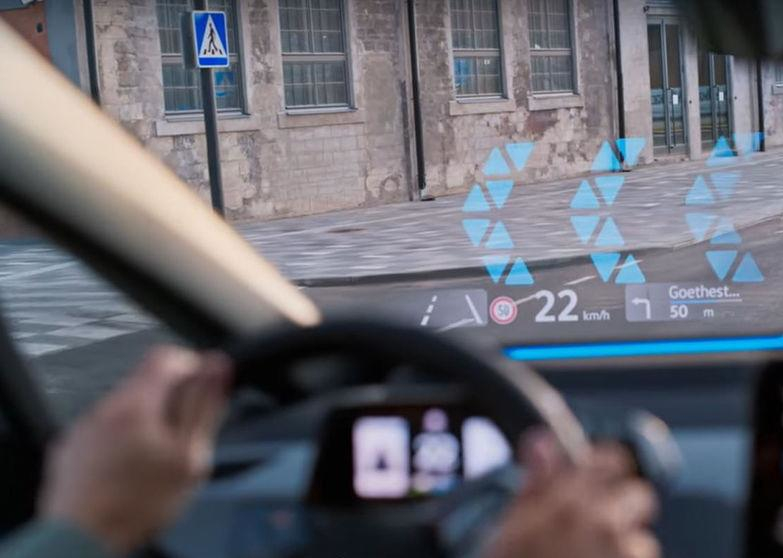
\includegraphics[width=0.8\textwidth]{images/Augmented-Reality-Head-Up-Display.jpg}
    \caption{Head-up Display.}
    \label{fig:figure18}
\end{figure}
\newpage
\subsection{Smart-Glasses}
Gli smart-glasses (Figura \ref{fig:figure19}) sono occhiali che permettono all’utente di ricevere informazioni direttamente sulle lenti.
I primi modelli potevano eseguire solo attività base, delegando il carico computazionale a dispositivi mobili come smartphone e tablet, connessi tramite Bluetooth, oggi invece sono in grado di eseguire vere e proprie applicazioni autonomamente.

\begin{figure}[H]
    \centering
    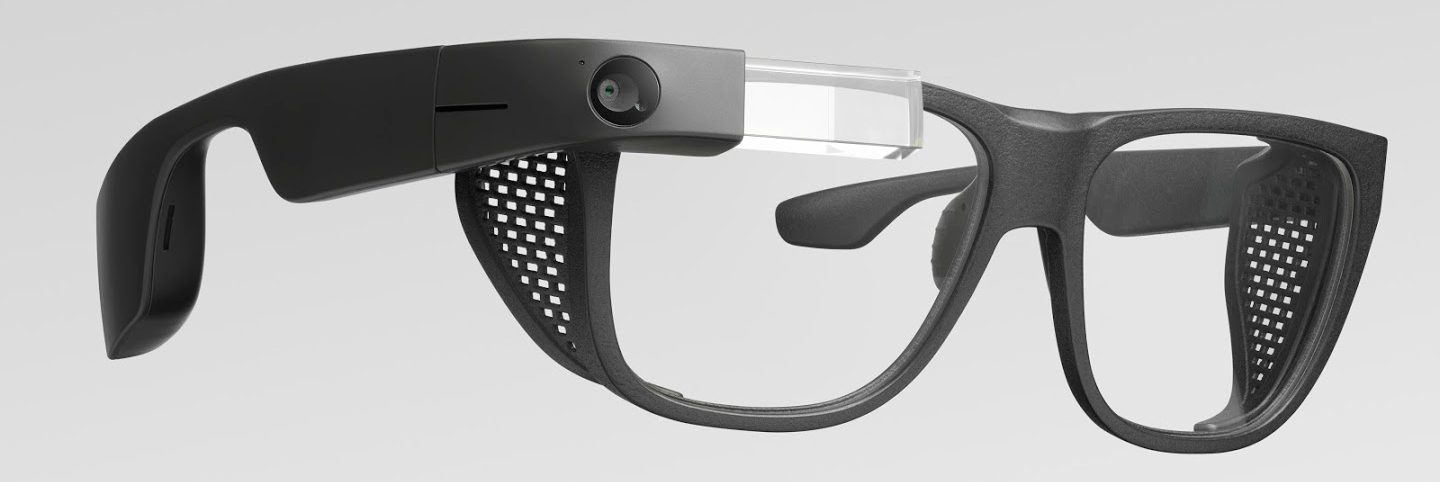
\includegraphics[width=0.7\textwidth]{images/smart-glass.jpg}
    \caption{Google Glass.}
    \label{fig:figure19}
\end{figure}

\subsection{Dispositivi Mobili}
La categoria dei dispositivi mobili riguarda device come smartphone e tablet che eseguono Android o iOS.
Questi apparati non sono stati progettati appositamente per esperienze AR, tuttavia negli ultimi anni sono state sviluppate piattaforme come Google ARCore e Apple ARKit, che rendono possibile lo sviluppo di applicazioni AR sfruttando la sensoristica dei device.

I dispositivi mobile sfruttano una tecnologia di tipo \textit{video see-through}.
La videocamera cattura il mondo reale dal punto di vista dell’utente, in fase di elaborazione vengono aggiunte le informazioni digitali e infine il risultato viene riportato sul display del device (Figura \ref{fig:figure110}).
\begin{figure}[H]
    \centering
    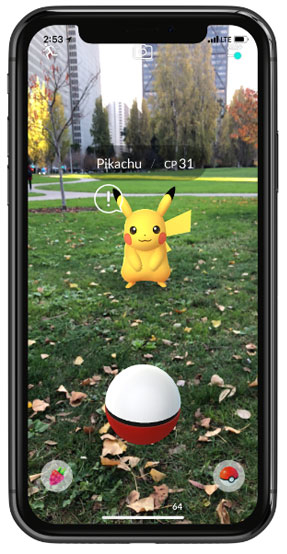
\includegraphics[scale=0.5]{images/pokemon_go.jpg}
    \caption{Applicazione AR in esecuzione su un dispositivo mobile.}
    \label{fig:figure110}
\end{figure}

\section{Framework di Sviluppo MR}\label{sec:Sezione1.5}
Per realizzare applicazioni MR è necessario considerare le piattaforme e i dispositivi di destinazione, questo perché oggi sono disponibili vari framework di sviluppo, realizzati per piattaforme specifiche o per garantire l'interoperabilità fra i diversi sistemi attualmente in commercio.

\subsection{Microsoft Mixed Reality Toolkit}
Mixed Reality Toolkit (MRTK) \footnote{https://github.com/Microsoft/MixedRealityToolkit-Unity} è un progetto gestito da Microsoft che fornisce un set di componenti e funzionalità che consentono lo sviluppo di app di realtà mista multipiattaforma.
Per sfruttare le funzionalità offerte da questo framework è necessario integrarlo in ambienti di sviluppo come Unity o Unreal Engine.
MRTK è modulare, questo significa che è possibile installare nell'ambiente di sviluppo solo i componenti necessari per lo sviluppo dell’applicazione; in questo modo la dimensione del progetto rimane contenuta. Inoltre, poiché è costruito con oggetti scriptabili, è anche possibile sostituire i componenti inclusi con i propri, per supportare altri servizi, sistemi e piattaforme. 
MRTK è in continuo sviluppo, vengono introdotte nuove funzionalità e risolti problemi costantemente, allo stesso tempo alcune funzionalità vengono deprecate.
MRTK viene impiegato nello sviluppo di applicazioni AR per HoloLens 1 e 2.

\subsection{Apple ARKit}
ARKit \footnote{https://developer.apple.com/augmented-reality/arkit/} è la piattaforma di realtà aumentata (AR) di Apple per dispositivi iOS.
Questa piattaforma di sviluppo che consente agli sviluppatori di app di creare rapidamente e facilmente esperienze AR nelle loro app e giochi. Utilizza la fotocamera, i processori e i sensori di movimento del dispositivo per creare interazioni coinvolgenti.

Per creare una corrispondenza tra spazio reale e virtuale, ARKit utilizza una tecnica chiamata Visual Inertial Odometry. Questo processo combina le informazioni provenienti dall'hardware di rilevamento del movimento del dispositivo iOS con l'analisi della visione artificiale della scena visibile dalla fotocamera del dispositivo. ARKit riconosce i feature point nell'immagine della scena, tiene traccia delle differenze nelle posizioni di tali punti tra i fotogrammi video e confronta tali informazioni con i dati di rilevamento del movimento. Il risultato è un modello ad alta precisione della posizione e del movimento del dispositivo.

Il monitoraggio del mondo analizza e comprende anche i contenuti di una scena. Vengono utilizzati metodi di ray-casting per trovare superfici del mondo reale corrispondenti a un punto nell'immagine della telecamera. Abilitando l'impostazione planeDetection nella configurazione della sessione, ARKit rileva le superfici piane nell'immagine della telecamera e ne riporta la posizione e le dimensioni. È anche possibile utilizzare i risultati ray-cast o i piani rilevati per posizionare o interagire con il contenuto virtuale nella scena. 

\subsection{Google ARCore}
ARCore \footnote{https://developers.google.com/ar/} è un framework di sviluppo software sviluppato da Google che consente di creare applicazioni di realtà aumentata.
La tecnologia di tracciamento del movimento di ARCore utilizza la fotocamera del telefono per identificare i feature point e tiene traccia di come questi punti si muovono nel tempo. Con una combinazione del movimento di questi punti e delle letture dei sensori inerziali del telefono, ARCore determina sia la posizione che l'orientamento del telefono mentre si muove nello spazio.

Oltre a identificare i punti chiave, ARCore può rilevare superfici piane, come un tavolo o il pavimento, e può anche stimare l'illuminazione media nell'area circostante. Queste capacità si combinano per consentire ad ARCore di costruire la propria comprensione del mondo che lo circonda.

La comprensione di ARCore del mondo reale consente di posizionare oggetti, annotazioni o altre informazioni in un modo che si integra perfettamente con il mondo reale.
Grazie al rilevamento del movimento l'utente può spostarsi e visualizzare gli oggetti virtuali da qualsiasi angolazione.

ARCore fornisce SDK per molti degli ambienti di sviluppo più diffusi. Questi SDK forniscono API native per tutte le funzionalità AR essenziali come il rilevamento del movimento, la comprensione dell'ambiente e la stima della luminosità. Con queste funzionalità è possibile creare esperienze AR completamente nuove o migliorare le app esistenti con funzionalità AR.

\subsection{OpenXR}
OpenXR \footnote{https://www.khronos.org/OpenXR/} è un’Application Program Interface (API), ad alte prestazioni, royalty-free (licenza che permette all'utente di utilizzare la risorsa senza limiti di tempo e spazio senza dover sostenere ulteriori costi) sviluppata da Khronos, la quale si occupa di fornire un accesso nativo alle piattaforme e ai dispositivi di Augmented, Mixed e Virtual Reality. Il termine XR, infatti, sta per eXtended Reality e comprende descritte nella sezione \ref{sec:Sezione1.2}.
OpenXR dal punto di vista del programmatore, consiste in un insieme di funzioni che si interfacciano con una runtime, per eseguire operazioni comunemente richieste come ad esempio: accedere al controller o allo stato della periferica utilizzata, ottenere le posizioni di tracciamento dei dispositivi di input o della testa dell’utente e inviare frame renderizzati.

OpenXR mira a semplificare lo sviluppo del software AR/VR, consentendo alle applicazioni di raggiungere una gamma più ampia di piattaforme hardware senza dover trasferire o riscrivere il codice e, successivamente, consentendo ai fornitori di piattaforme che supportano OpenXR di accedere a più applicazioni.

Senza uno standard multipiattaforma, le applicazioni e gli engine VR/AR devono utilizzare le API proprietarie di ciascuna piattaforma. I nuovi dispositivi di input richiedono l'integrazione di driver personalizzati (Figura \ref{fig:figure111a}).

OpenXR fornisce accesso multipiattaforma e ad alte prestazioni direttamente alle diverse runtime dei dispositivi XR su più piattaforme. OpenXR consente l'esecuzione di applicazioni ed engine, incluso WebXR, su qualsiasi sistema che esponga le API OpenXR (Figura \ref{fig:figure111b}).

\begin{figure}[t]
    \centering
    \begin{subfigure}{0.6\textwidth}
        \centering
        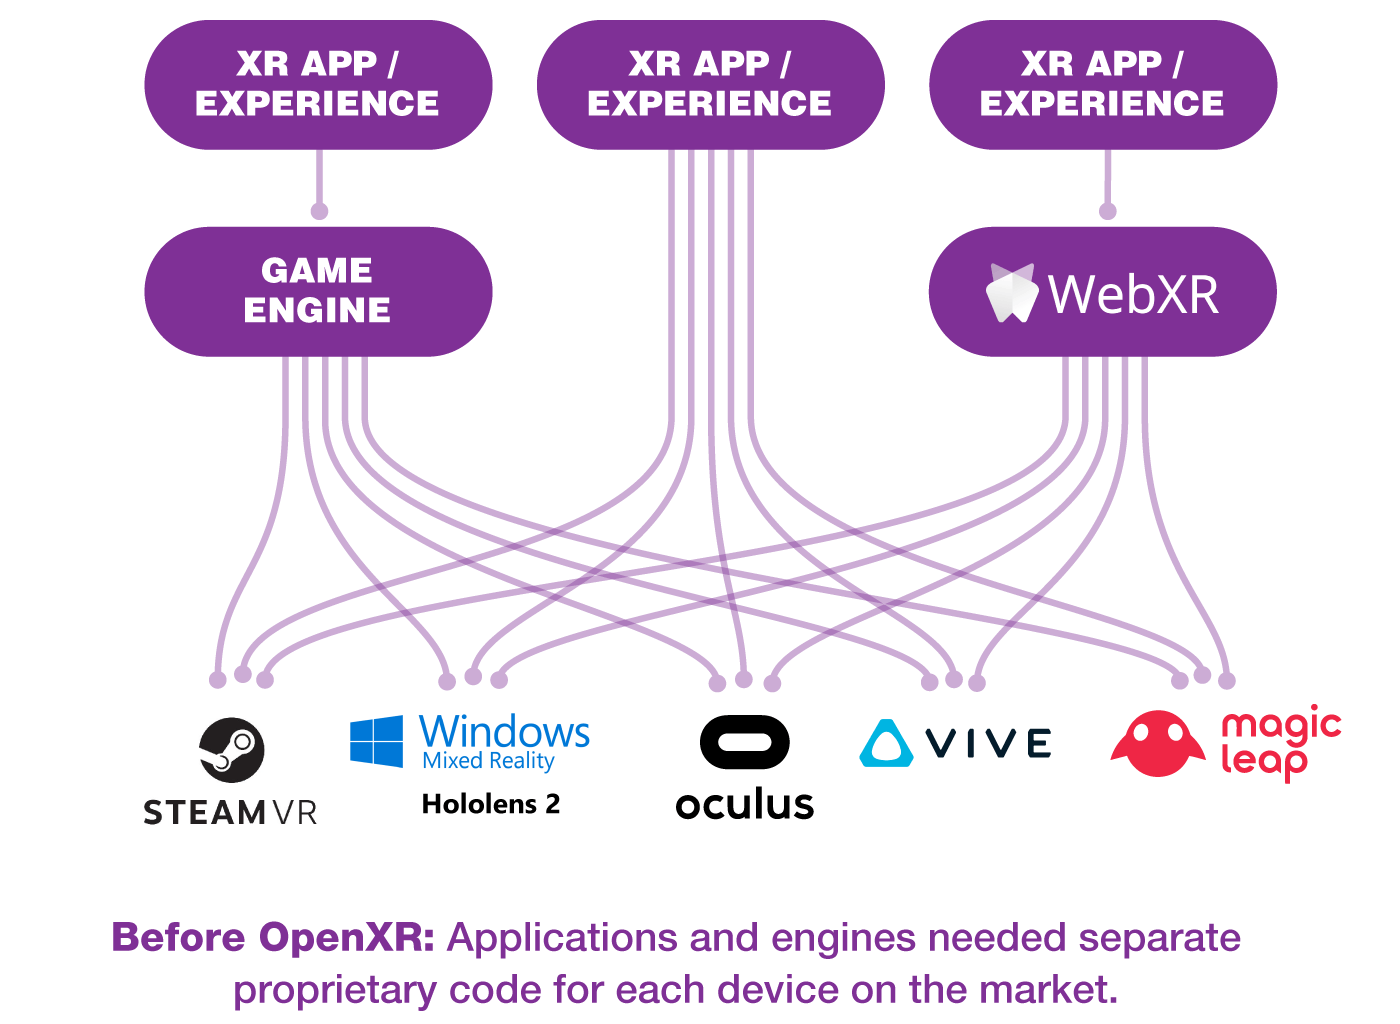
\includegraphics[width=\textwidth]{images/OpenXR-Before_3.png}
        \caption{Sviluppo senza OpenXR}
        \label{fig:figure111a}
    \end{subfigure}
    \begin{subfigure}{0.6\textwidth}
        \centering
        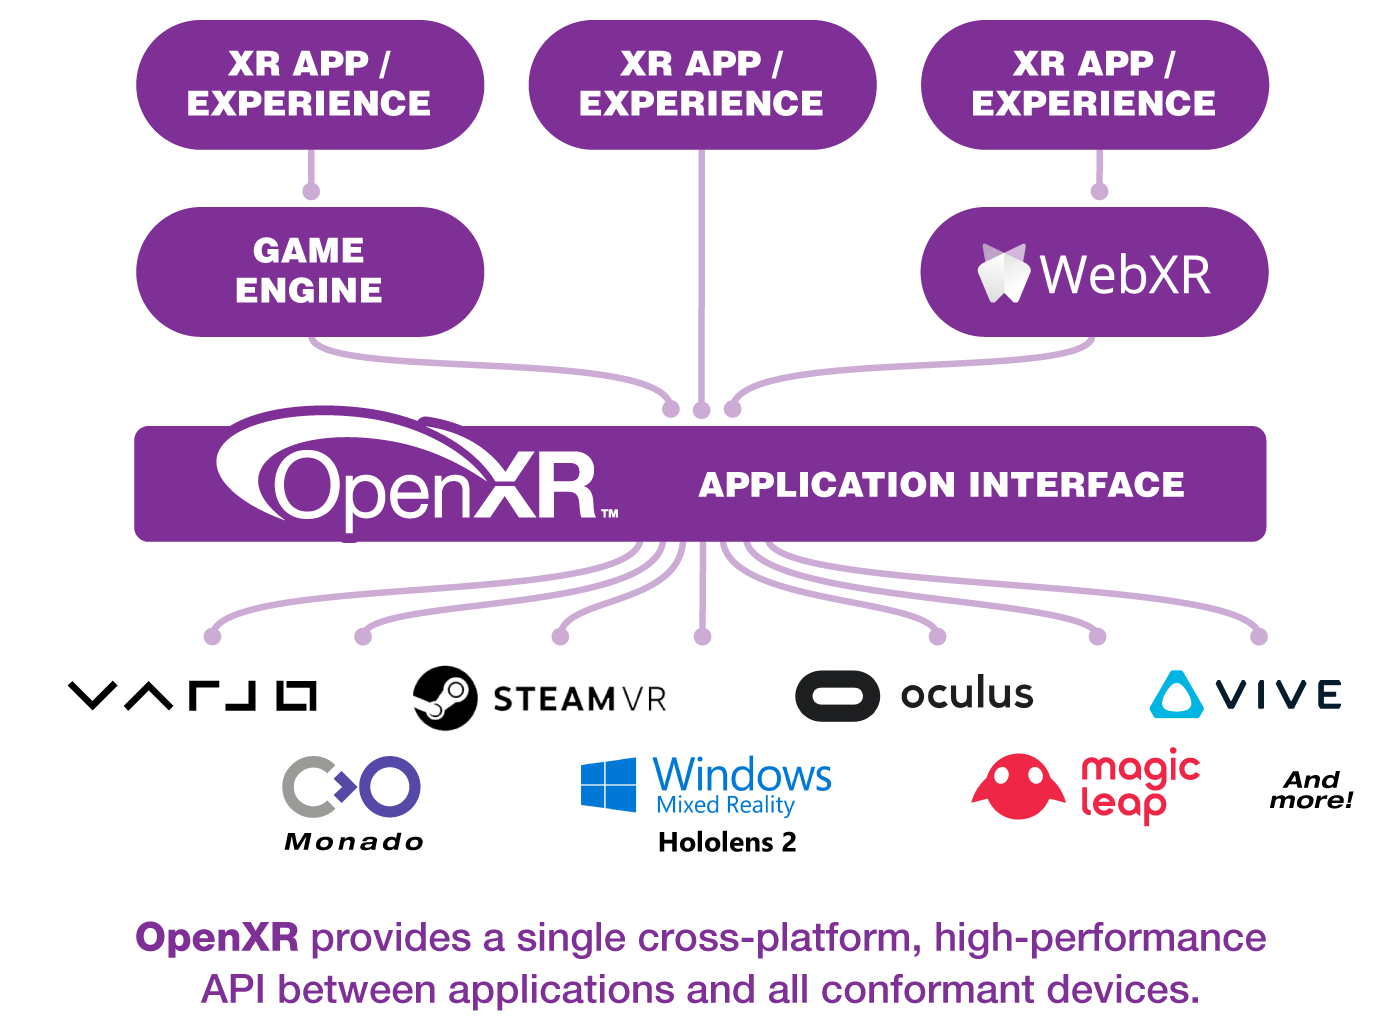
\includegraphics[width=\textwidth]{images/OpenXR-After_3.png}
        \caption{Sviluppo con OpenXR}
        \label{fig:figure111b}
    \end{subfigure}
       \caption{Problema della frammentazione risolto da OpenXR}
       \label{fig:figure111}
\end{figure}

\subsection{Vuforia}
Vuforia \footnote{https://developer.vuforia.com/} è un framework di sviluppo per applicazioni AR ed è stato introdotto da Qualcomm, un'azienda inizialmente specializzata nella ricerca e nello sviluppo dei mezzi di comunicazione wireless e dei microchip elettronici SoC.

Nel cuore della piattaforma si trova una libreria QCAR scritta in C++, che supporta vari tipi di target (image cube, cuboid, cylinder, word target e frame marker) e funzionalità di rendering dell'immagine. I target in Vuforia sono, fondamentalmente, oggetti reali, che possono essere sfruttati dalla applicazione per posizionare oggetti virtuali o per condividere sistemi di coordinate con altri dispositivi.

Vuforia dispone anche di Extended Tracking: dopo il primo rilevamento il dispositivo mantiene il tracciamento anche quando il target non è più visibile, quindi una volta trovato il target l’utente è libero di muoversi nell’ambiente.

Quella che segue è una descrizione di alto livello del processo di rilevazione del target: 
\begin{enumerate}
\item Il Tracker di Vuforia Engine riconosce il target.
\item Il tracciamento del target viene quindi inizializzato. 
\item La posizione e la rotazione del target vengono analizzate per fornire una stima della posa al dispositivo. 
\item Vuforia Engine trasforma la posa del target nel sistema di coordinate del dispositivo. 
\item Il dispositivo assume il controllo nel momento in cui il target non è più visibile.
Quando il target compare nuovamente nel campo visivo Vuforia esegue nuovamente il tracciamento. 
\end{enumerate}

\chapter{Microsoft HoloLens 2}
Il primo sistema operativo olografico al mondo è stato introdotto da Microsoft nel 2015 appositamente per dispositivi HoloLens.
Originariamente noto come \textit{Windows Holographic}, questa variante del sistema operativo Windows ha fornito una piattaforma di realtà mista che potesse essere sperimentata dagli sviluppatori e ha permesso di integrare le app universali di Windows esistenti in questo nuovo ambiente.
Successivamente, Microsoft ha consentito ai visori compatibili di utilizzare un ambiente \textit{Windows Mixed Reality} all'interno di Windows stesso, integrando parte dell'esperienza utente introdotta in precedenza da Microsoft HoloLens.

\section{Specifiche Tecniche del Device}\label{sec:Sezione2.1}

Come detto in precedenza, HoloLens 2 è un visore per la realtà mista annunciato da Microsoft nel Mobile World Congress del 2019.
Questa nuova versione va a rimpiazzare la prima generazione di HoloLens, introdotta nel 2016.
Di seguito vengono presentate le caratteristiche hardware del dispositivo (Figura \ref{fig:figure2}), comparate anche a quelle del suo predecessore.

\begin{figure}[t]
    \centering
    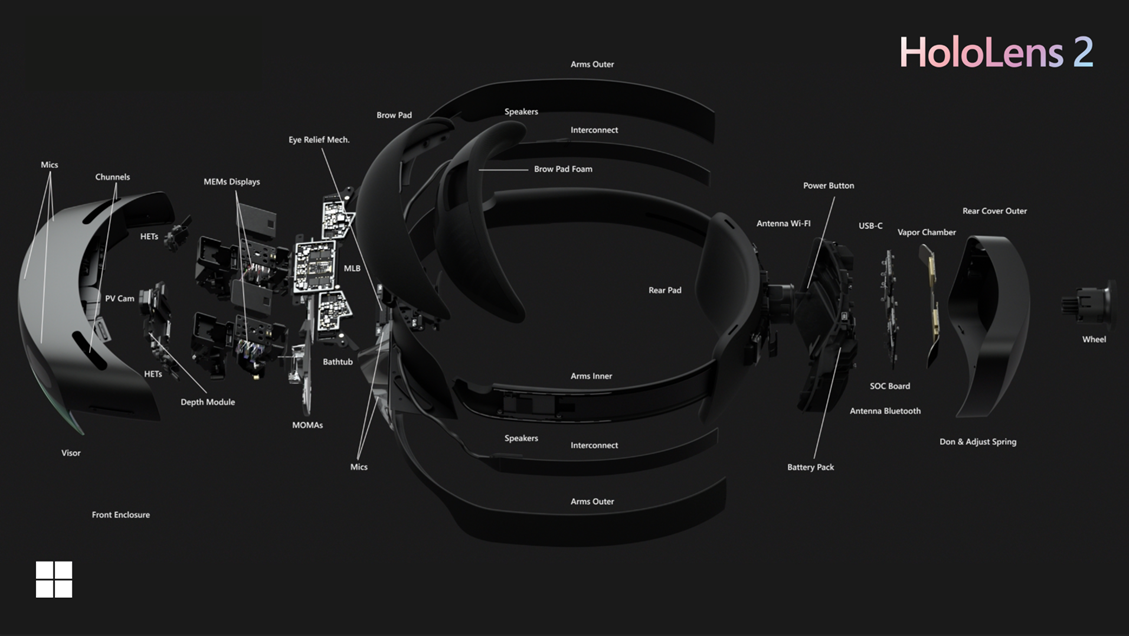
\includegraphics[width=\textwidth]{images/hololens2-breakdown.png}
    \caption{Componenti di HoloLens 2.}
    \label{fig:figure2}
\end{figure}

HoloLens 2 vanta un campo visivo ampliato e una risoluzione ottica notevolmente aumentata, passando da circa 720p a 2K di risoluzione per occhio. Ciò consente agli utenti di visualizzare ologrammi molto più dettagliati e di vederli da angoli più ampi, piuttosto che dover rimanere concentrati su punti molto specifici.

\begin{center}
    \begin{tabular}{ p{6cm} p{7cm} }
        \hline
        \multicolumn{2}{c}{\textbf{Display}} \\
        \hline
        \textbf{Optics} & See-through holographic lenses (waveguides)\\
        \hline
        \textbf{Holographic resolution} & 2k 3:2 light engines\\
        \hline
        \textbf{Holographic density} & 2.5k radiants (light points per radian)\\
        \hline
        \textbf{Eye-based rendering} & Display optimization for 3D eye position\\
        \hline
    \end{tabular}
\end{center}

    HoloLens 2 dispone di un comparto sensoristico all'avanguardia, utilizzato per tracciare mani e occhi dell'utente e per stabilire la sua posizione nell'ambiente.

\begin{center}
    \begin{tabular}{ p{6cm} p{7cm} }
        \hline
        \multicolumn{2}{c}{\textbf{Sensors}} \\
        \hline
        \textbf{Head tracking} & 4 visible light cameras\\
        \hline
        \textbf{Eye tracking} & 2 Infrared (IR) cameras\\
        \hline
        \textbf{Depth} & 1-MP Time-of-Flight depth sensor\\
        \hline
        \textbf{Inertial measurement unit} & Accelerometer, gyroscope, magnetometer\\
        \hline
        \textbf{Camera} & 8-MP stills, 1080p30 video\\
        \hline
    \end{tabular}
\end{center}

Esattamente come il display, gli speaker di HoloLens 2 sono additivi, questo significa che l'utente è in grado di percepire sia i suoni prodotti dal device che quelli provenienti dall'ambiente.
    
\begin{center}
    \begin{tabular}{ p{6cm} p{7cm} }
        \hline
        \multicolumn{2}{c}{\textbf{Audio}} \\
        \hline
        \textbf{Microphone array} & 5 channels\\
        \hline
        \textbf{Speakers} & Built-in spatial sound\\
        \hline
    \end{tabular}
\end{center}

Grazie al processore Snapdragon 850 e ai moduli per le comunicazioni wireless (Wi-Fi e Bluetooth), HoloLens 2 è in grado di collegarsi alla rete per navigare nel web o per partecipare a esperienze condivise con altri dispositivi.

\begin{center}
    \begin{tabular}{ p{6cm} p{7cm} }
        \hline
        \multicolumn{2}{c}{\textbf{Compute and connectivity}} \\
        \hline
        \textbf{System on chip} & Qualcomm Snapdragon 850 Compute Platform\\
        \hline
        \textbf{Holographic processing unit} & Second-generation custom-built holographic processing unit\\
        \hline
        \textbf{Memory} & 4-GB LPDDR4x system DRAM\\
        \hline
        \textbf{Storage} & 64-GB UFS 2.1\\
        \hline
        \textbf{Wi-Fi} & 802.11ac 2x2\\
        \hline
        \textbf{Bluetooth} & 5.0\\
        \hline
        \textbf{USB} & USB Type-C DRP\\
        \hline
    \end{tabular}
\end{center}

Un'altra area in cui HoloLens 2 migliora rispetto al suo predecessore è l'interazione, con l'intelligenza artificiale integrata che misura il modo in cui gli utenti manipolano gli ologrammi proiettati dal visore.

\begin{center}
    \begin{tabular}{ p{6cm} p{7cm} }
        \hline
        \multicolumn{2}{c}{\textbf{Device capabilities}} \\
        \hline
        \textbf{Hand tracking} & Two-handed fully articulated model, direct manipulation\\
        \hline
        \textbf{Eye tracking} & Real-time tracking\\
        \hline
        \textbf{Voice} & Command and control on-device; Cortana natural language with internet connectivity\\
        \hline
        \textbf{Six Degrees of Freedom tracking} & World-scale positional tracking\\
        \hline
        \textbf{Spatial mapping} & Real-time environment mesh\\
        \hline
        \textbf{Mixed reality capture} & Mixed hologram and physical environment photos and videos\\
        \hline
    \end{tabular}
\end{center}

\section{Architettura di un'Applicazione HoloLens 2}\label{sec:Sezione2.2}

\subsection{Sistemi di Coordinate}
Tutte le applicazioni di grafica 3D utilizzano sistemi di coordinate cartesiane per stabilire posizione e orientamento degli oggetti virtuali.
Nella realtà mista, le applicazioni ragionano su sistemi di coordinate virtuali e fisici.
In Windows un sistema di coordinate che ha un significato reale nel mondo fisico viene definito sistema di coordinate spaziali.
I sistemi di coordinate spaziali esprimono i loro valori di coordinate in metri. Ciò significa che gli oggetti posizionati a due unità di distanza sull'asse X, Y o Z appariranno a due metri di distanza l'uno dall'altro quando renderizzati in realtà mista.
Sapendo questo, è possibile eseguire il rendering di oggetti e ambienti su scala reale.
In generale, i sistemi di coordinate cartesiane possono essere \textit{right-handed} (destrorsi) o \textit{left-handed} (sinistrorsi).
I sistemi di coordinate spaziali su Windows sono sempre right-handed, il che significa che l'asse X positivo punta a destra, l'asse Y positivo punta verso l'alto e l'asse Z positivo punta verso il visore.

\subsection{Ologrammi}
Gli ologrammi sono entità digitali poste all’interno di un ambiente fisico e possono rappresentare elementi reali (come una sedia o un tavolo) o immaginari.
HoloLens, grazie ai suoi sistemi di I/O, fornisce all’utente la possibilità di interagire con gli ologrammi come se fossero concreti.
Un ologramma può anche interagire con l'ambiente circostante. Ad esempio, è possibile posizionare una palla olografica che rimbalza ed emette un suono nel momento in cui colpisce il suolo.

\begin{figure}[t]
    \centering
    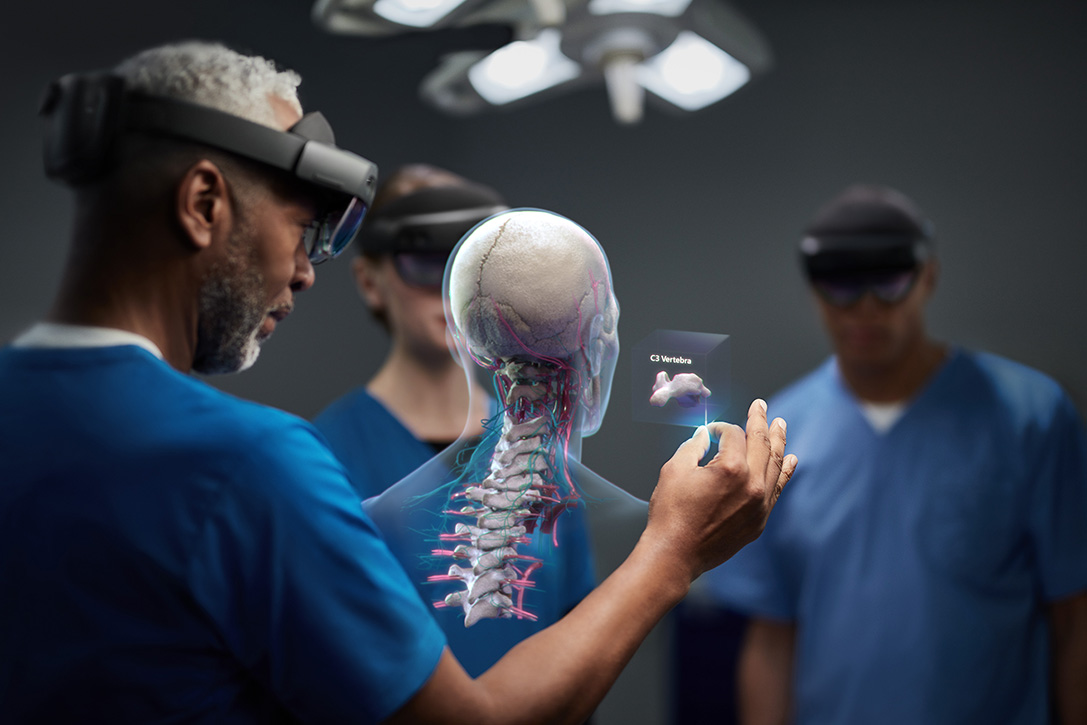
\includegraphics[width=\textwidth]{images/hologram.jpg}
    \caption{Grazie ad HoloLens l'utente può interagire con gli ologrammi}
    \label{fig:figure21}
\end{figure}

Gli ologrammi che vengono renderizzati da HoloLens appaiono nel frame olografico, direttamente davanti agli occhi dell’utente. Per effettuare il rendering HoloLens usa un display additivo, che aggiunge luce a una determinata area del frame, il che significa che è possibile vedere sia la luce emessa dal display che la luce del mondo circostante.

Gli ologrammi possono anche produrre suoni che sembrano provenire da un luogo specifico nell’ambiente. Su HoloLens, il suono proviene da due altoparlanti posizionati direttamente sopra le orecchie. Come il display olografico, gli altoparlanti sono additivi, quindi i nuovi suoni vengono introdotti senza occludere quelli provenienti dall'ambiente.

Gli ologrammi possono avere una posizione fissa all’interno dell’ambiente o seguire l’utente. Nel primo caso è anche possibile utilizzare le ancore per rendere la posizione degli ologrammi persistente anche attraverso diverse sessioni. 
Alcuni scenari invece richiedono che gli ologrammi rimangano facilmente individuabili o visibili durante la sessione. Ci sono due approcci di alto livello per questo tipo di posizionamento, chiamati \textit{display-locked} e \textit{body-locked}. 

Nel caso del display-locked i contenuti vengono fissati sul display, questo approccio crea delle complicazioni, infatti il campo visivo dell’utente viene limitato. 

Con l’approccio body-locked l’ologramma si lega al corpo dell’utente, in questo modo è possibile muoversi e spostarsi senza perderlo di vista e allo stesso tempo il campo visivo rimane inalterato.

\subsection{Mappatura Spaziale}
La mappatura spaziale genera un modello 3D dell’ambiente chiamato \textit{mesh} (Figura \ref{fig:figure22}), consentendo di posizionare oggetti virtuali su superfici reali.
Uno degli usi principali della mesh creata dalla mappatura spaziale è quello di occludere gli ologrammi, che vengono percepiti come se fossero reali. 

L'occlusione fornisce anche informazioni all'utente;
quando un ologramma viene occluso da una superficie del mondo reale, questo fornisce un feedback visivo aggiuntivo sulla sua posizione in quell’ambiente.
Inoltre, l'occlusione può anche nascondere in modo utile le informazioni all'utente; occludere ologrammi dietro i muri può ridurre il disordine visivo. 

La mappatura spaziale è utile anche nel momento in cui si vuole applicare qualsiasi tipo di forza fisica agli ologrammi, sfruttando la mesh infatti è possibile farli collidere con gli ostacoli presenti nell’ambiente.
In alcuni casi, ad esempio se sono presenti superfici in vetro o riflettenti, la mesh potrebbe essere imprecisa e non corrispondere con l’ambiente, di conseguenza le collisioni degli ologrammi potrebbero essere inaccurate. 

L'archiviazione, il rendering e l'elaborazione delle mesh possono consumare notevoli risorse di calcolo e di archiviazione.
Pertanto, ogni applicazione dovrebbe adottare uno schema di caching appropriato alle proprie esigenze, determinando quali mesh mantenere, quali scartare e quando aggiornare quelle salvate.

\begin{figure}[t]
    \centering
    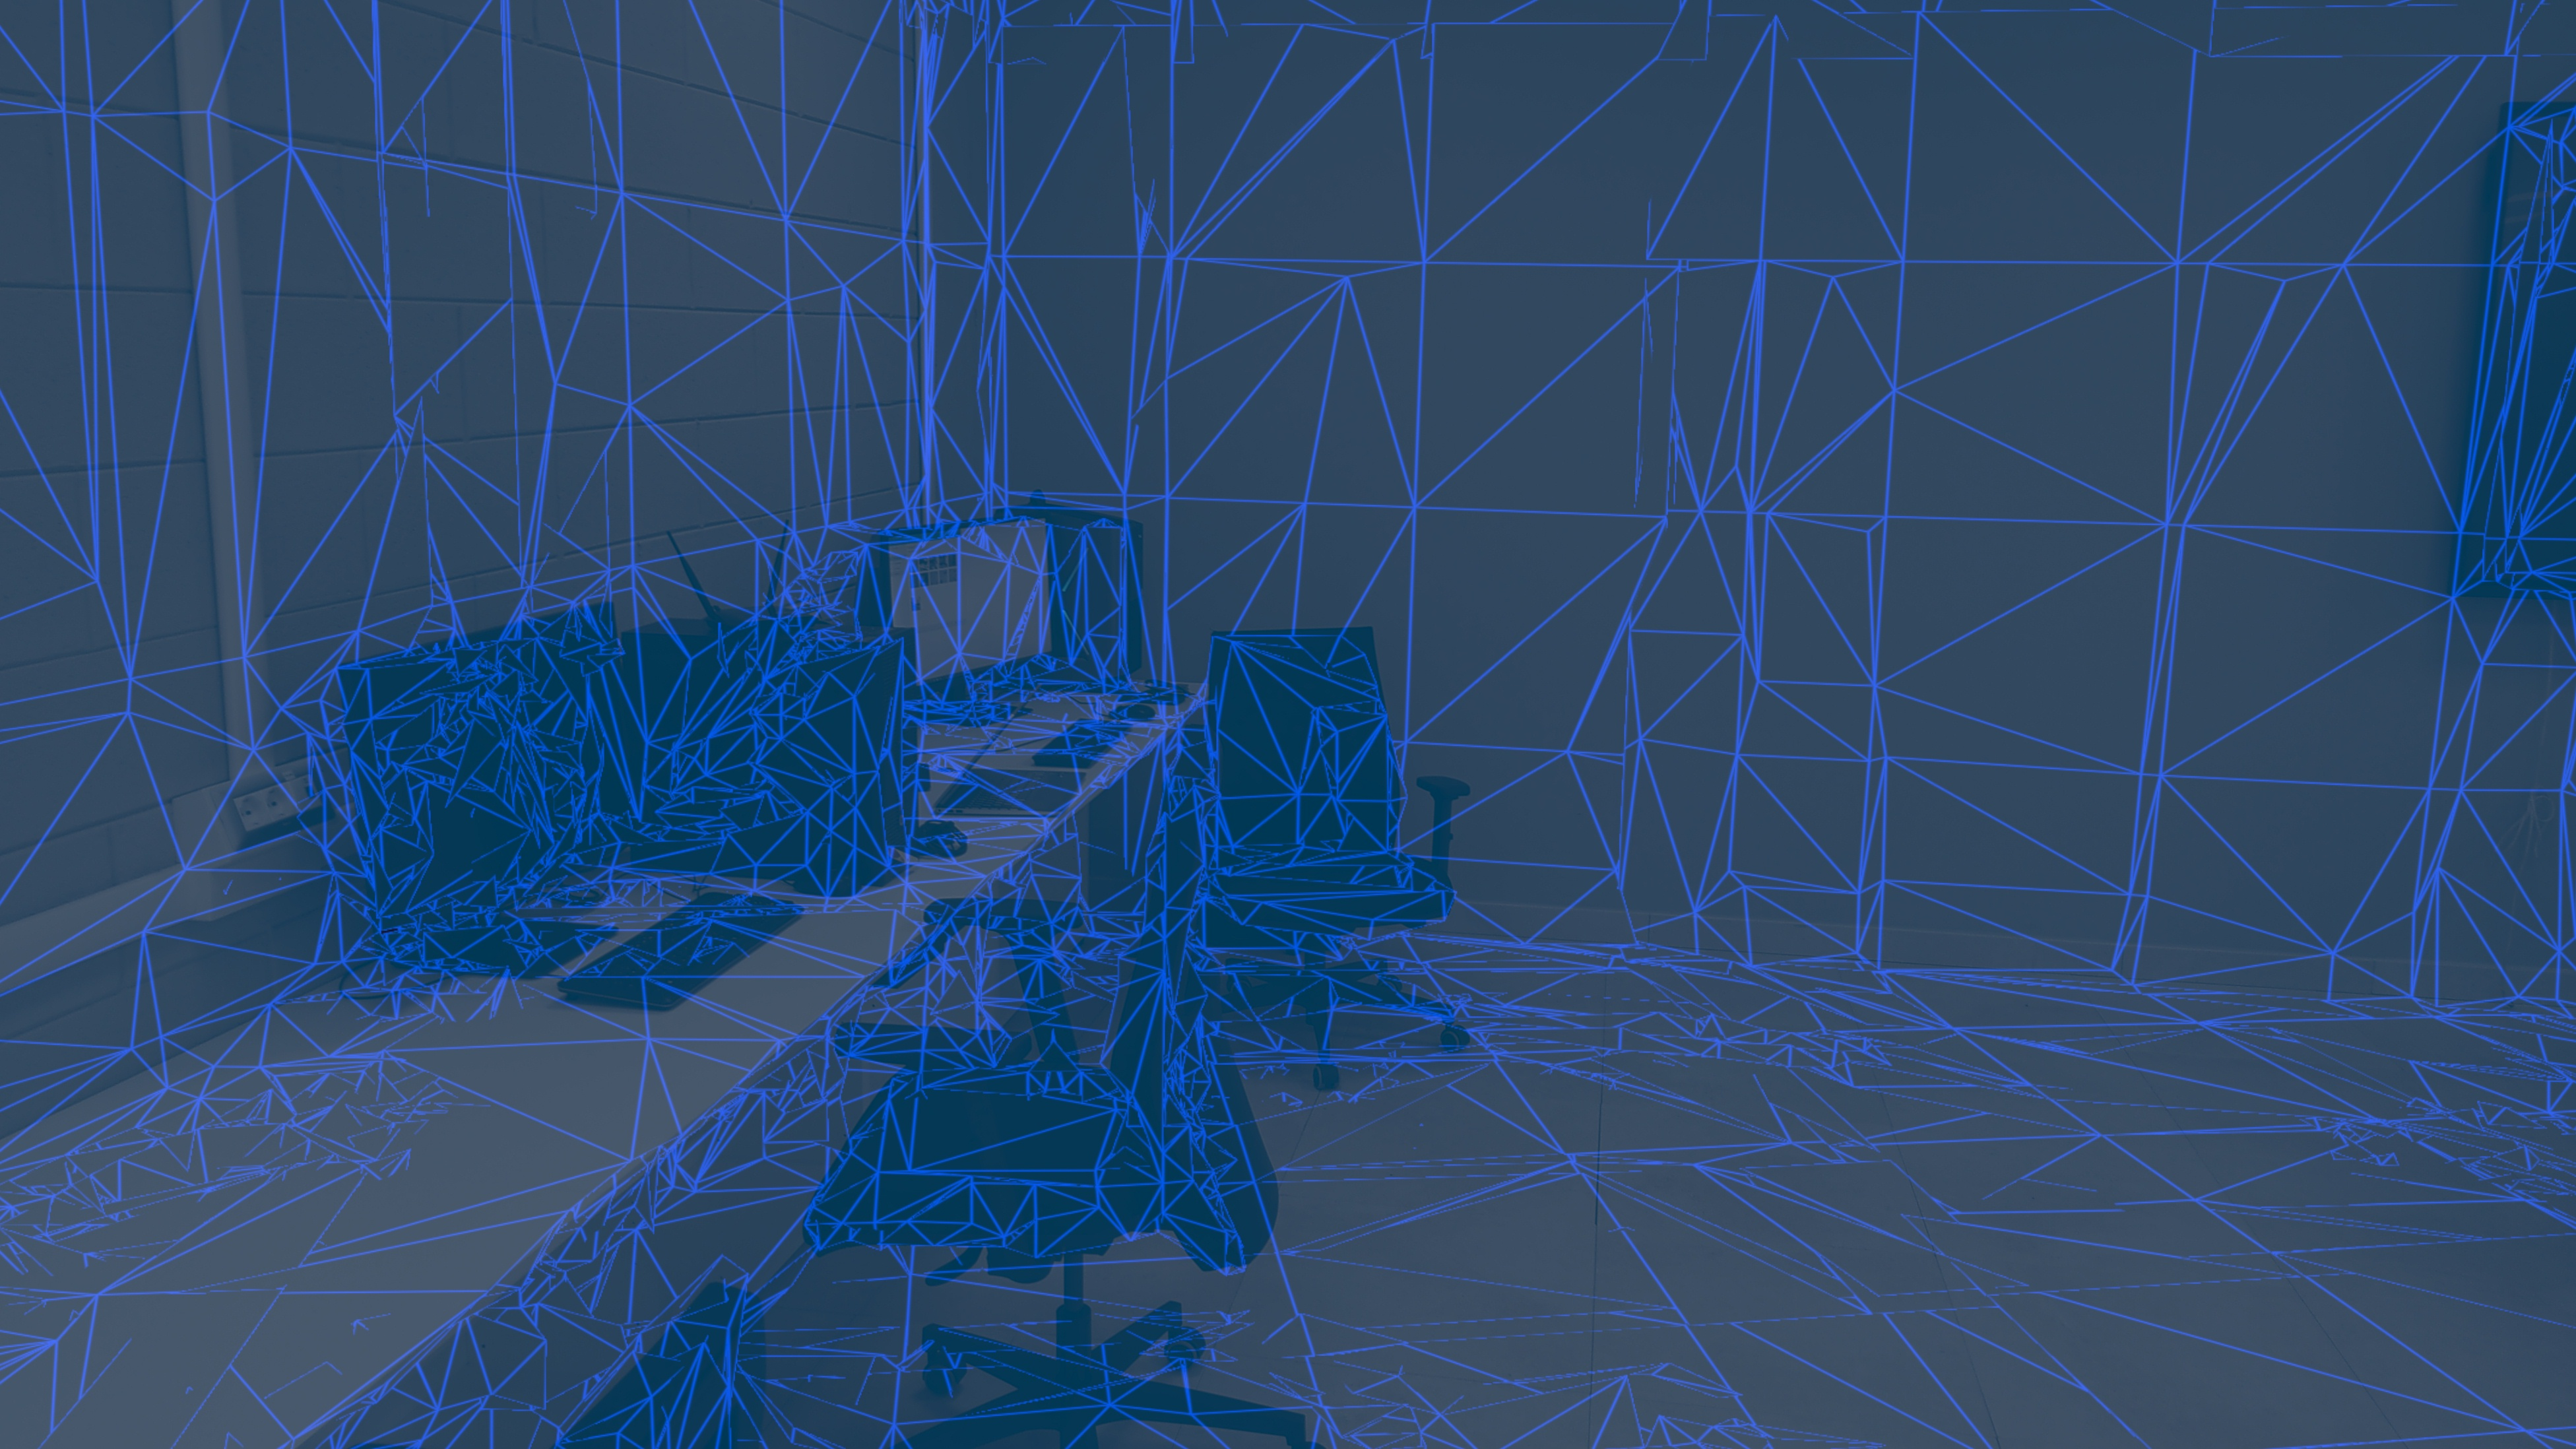
\includegraphics[width=\textwidth]{images/spatial-mapping.jpg}
    \caption{Mesh di una stanza, generata da HoloLens 2.}
    \label{fig:figure22}
\end{figure}

\subsection{Ancore}
Un’ancora rappresenta un punto nel mondo del quale il sistema tiene traccia nel tempo. Ogni ancora ha un sistema di coordinate regolabile, basato su altre ancore o sistemi di riferimento, per garantire che gli ologrammi ancorati rimangano esattamente al loro posto. È anche possibile mantenere e condividere ancore tra le sessioni dell'applicazione e tra diversi dispositivi: 

Salvando le ancore su disco e caricandole di nuovo in un secondo momento, l'applicazione può calcolare la stessa posizione nel mondo reale in più sessioni dell'applicazione su un singolo HoloLens. 

Usando i servizi Azure è possibile condividere un'ancora in cloud con più dispositivi HoloLens, iOS e Android. Facendo in modo che ogni dispositivo esegua un ologramma utilizzando la stessa ancora spaziale, gli utenti vedranno l'ologramma apparire nello stesso posto nel mondo reale. Ciò consente esperienze condivise in tempo reale. 

Le ancore condivise in cloud possono persistere anche in modo asincrono, quindi i vari dispositivi presenti nell’ambiente possono osservare e interagire con lo stesso ologramma in momenti diversi. 

Gli ologrammi che vengono ancorati purtroppo non possono essere spostati o ruotati, quindi ogni volta che si desidera interagire con un ologramma ancorato bisogna prima eliminare l’ancora, per poi crearla nuovamente nel momento in cui termina l’interazione.
Questo pone un forte limite alle esperienze condivise che sfruttano questa funzionalità;
infatti se in un ambiente sono presenti più utenti e uno di questi interagisce con un ologramma ancorato gli altri non sono in grado di vedere la fase d'interazione.

\subsection{Hand Tracking e Gaze}
La manipolazione diretta è un modello di input primario su HoloLens 2, che usa il nuovo sistema di rilevamento della mano.
HoloLens 2 è in grado di riconoscere mani e dita dell'utente (Figura \ref{fig:figure24a}) e di rilevare le collisioni con gli ologrammi, quindi è possibile interagire con questi come se fossero reali.
È anche possibile sfruttare l'indice della mano come puntatore 3D (gaze, Figura \ref{fig:figure24b}), in questo modo è possibile interagire con gli ologrammi più distanti senza doversi spostare; solitamente in un'applicazione HoloLens 2 i gaze sono due, uno per ogni mano.
Il gaze può anche essere utilizzato sfruttando gli occhi, lasciando così le mani libere.
Grazie a questa funzionalità l'utente può "fissare" l'ologramma alla testa, di conseguenza l'oggetto si muoverà e ruoterà nell'ambiente seguendo la testa dell'utente.
Le possibili interazioni con gli ologrammi sono varie, ad esempio sfruttando una mano sola si può puntare il gaze su un ologramma, unire indice e pollice (air tap) e spostare la mano nella direzione in cui si vuole posizionare l'ologramma.
Se invece si vuole ridimensionare un ologramma è necessario usare tutte e due le mani, in questo caso bisogna puntare entrambi i gaze sull'ologramma ed eseguire la gesture air tap, allargando o avvicinando le mani l'ologramma si ridimensionerà.
Un altro tipo di interazione particolarmente interessante è la rotazione dell'oggetto, per ruotare un ologramma basta eseguire la stessa procedura descritta precedentemente per il movimento, solo che invece di spostare la mano bisogna ruotarla esattamente nel modo in cui si desidera ruotare l'oggetto.

\begin{figure}[H]
    \centering
    \begin{subfigure}{0.45\textwidth}
        \centering
        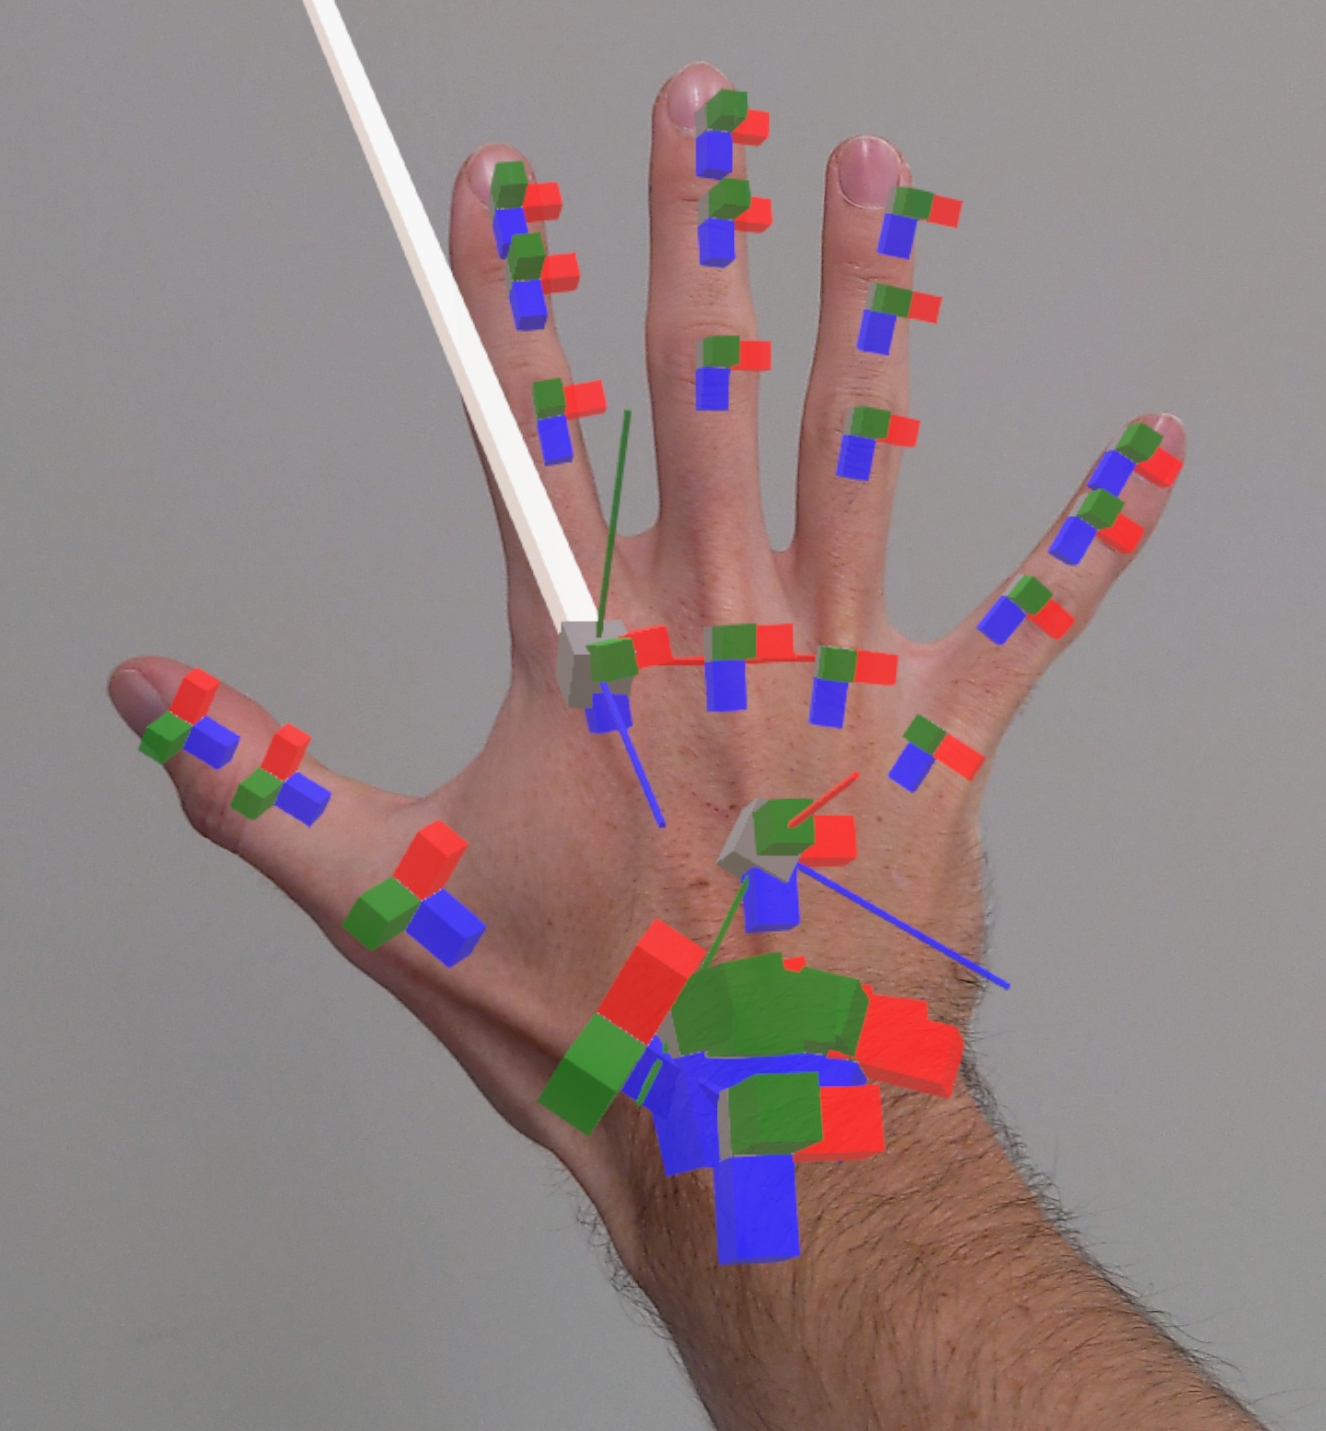
\includegraphics[width=\textwidth]{images/hand-tracking.jpg}
        \caption{Hand tracking.}
        \label{fig:figure24a}
    \end{subfigure}
    \begin{subfigure}{0.4\textwidth}
        \centering
        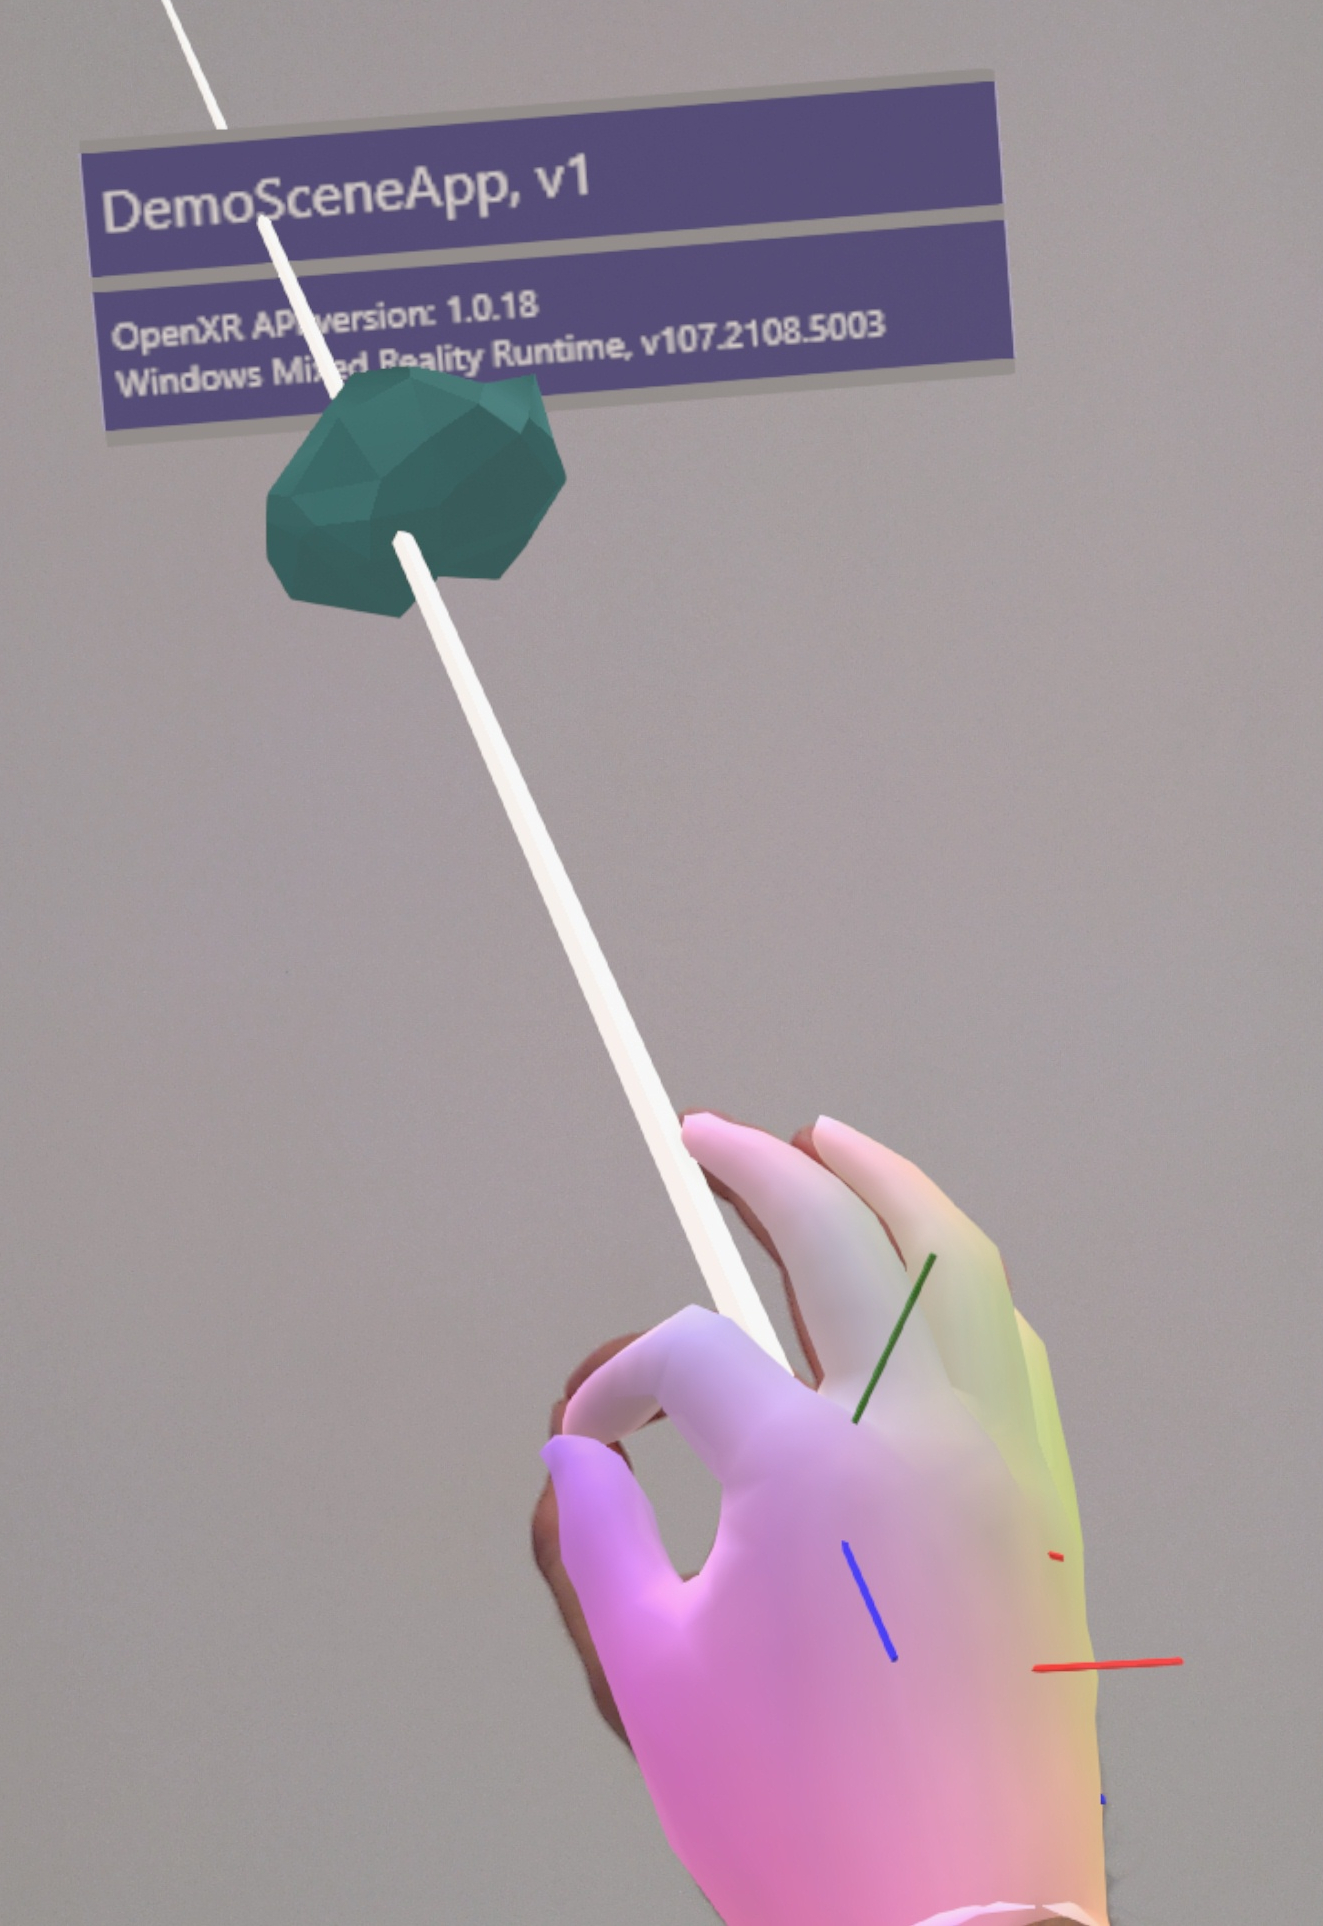
\includegraphics[width=\textwidth]{images/gaze.jpg}
        \caption{Gaze.}
        \label{fig:figure24b}
    \end{subfigure}
    \label{fig:figure24}
\end{figure}

\section{Strumenti di Sviluppo}\label{sec:Sezione2.3}
Per lo sviluppo di applicazioni HoloLens 2 esistono varie opzioni che si distinguono in base agli obiettivi e alle necessità degli sviluppatori:

\begin{itemize}
\item Unity è la piattaforma leader a livello mondiale per la creazione e l'utilizzo di contenuti 3D interattivi in tempo reale; il codice di runtime sottostante è C++, mentre lo scripting di sviluppo viene eseguito in C\#.
\item Unreal Engine 4 è un engine open source avanzato con supporto completo per la realtà mista sia in C++ che in Blueprints. 
\item Gli sviluppatori nativi che hanno esperienza nella scrittura di renderer 3D personalizzati possono creare un engine custom grazie ad OpenXR.
\item Gli sviluppatori Web che vogliono creare esperienze Web AR/VR per browser web possono usare WebXR.
\end{itemize}

Per il caso di studio si è scelto di utilizzare Unity in combinazione con il Mixed Reality Toolkit (MRTK) fornito da Microsoft, questo perché al momento è l'opzione migliore, sia dal punto di vista delle funzionalità offerte, che dalla stabilità.

MRTK per Unity è un progetto gestito da Microsoft che fornisce un set di componenti e funzionalità che consentono lo sviluppo di app di realtà mista multipiattaforma. 

MRTK è modulare, questo significa che è possibile installare in Unity solo i componenti necessari per lo sviluppo dell’applicazione; in questo modo la dimensione del progetto rimane contenuta. Inoltre, poiché è costruito con oggetti scriptabili, è anche possibile sostituire i componenti inclusi con i propri, per supportare altri servizi, sistemi e piattaforme. 

MRTK è in continuo sviluppo, vengono introdotte nuove funzionalità e risolti problemi costantemente, allo stesso tempo alcune funzionalità vengono deprecate, in base anche alle nuove versioni di Unity che vengono rilasciate. Ad oggi è possibile scegliere fra quattro opzioni, che si distinguono prevalentemente per la versione di Unity che si vuole utilizzare:

\begin{itemize}
\item L'attuale configurazione consigliata da Microsoft per HoloLens 2 e per lo sviluppo di Windows Mixed Reality è Unity 2020.3 LTS con il plug-in OpenXR più recente. 
\item Con Unity 2019 è possibile utilizzare plug-in XR integrato nell’ambiente di sviluppo. 
\item Con Unity 2021.2 il plug-in Windows XR è stato deprecato in favore di OpenXR, che quindi rimane l’unica opzione disponibile. 
\item Per Unity 2018.4 LTS è terminato il supporto di due anni e non vengono più rilasciati aggiornamenti.
\end{itemize}

I componenti del MRTK sono molti e offrono funzionalità di vario tipo: percezione ambiente, gestione dei sistemi di input e gestione delle ancore sono alcuni esempi.
La gestione di questi componenti all'interno di Unity viene affidata a dei profili specifici per ogni funzionalità.

\subsection{Sistema di Input}
Il sistema di input in MRTK consente di:
\begin{itemize}
    \item Rilevare input da una varietà di sorgenti, come controller 6DOF, mani o voce.
    \item Definire azioni astratte, come Select o Menu e associarle a diversi input.
    \item Impostare puntatori collegati ai controller per guidare i componenti dell'interfaccia utente tramite eventi del puntatore (focus e tap).
\end{itemize}

Gli input sono prodotti dagli Input Data Providers (Device Manager). Ogni provider corrisponde a una particolare fonte di input: Open VR, Windows Mixed Reality (WMR), Unity Joystick o Windows Speech, I provider vengono aggiunti al progetto tramite il profilo Registered Service Providers nel componente Mixed Reality Toolkit e producono eventi di input automaticamente quando sono disponibili le sorgenti di ingresso corrispondenti (ad esempio quando viene rilevato un controller WMR o collegato un gamepad).

Le azioni di input sono astrazioni intese a isolare la logica dell'applicazione dalle specifiche sorgenti di input. Può essere utile, ad esempio, definire un'azione Select e mapparla sul pulsante sinistro del mouse, un pulsante in un gamepad e un trigger in un controller 6DOF. È quindi possibile fare in modo che la logica dell'applicazione ascolti gli eventi dell'azione Seleziona in input invece di dover essere consapevole di tutti i diversi input che possono produrlo. Le azioni di input sono definite nel profilo delle azioni di input, che si trova all'interno del profilo Input System nel componente Mixed Reality Toolkit.

I controller vengono creati dai provider di input quando i dispositivi di input vengono rilevati e distrutti quando vengono persi o disconnessi. Il provider di input WMR, ad esempio, crea un controller WMR per dispositivi 6DOF e controller manuali WMR per le mani. Gli eventi di input generati dai controller includono l'eventuale azione di input associata.

I controller possono avere dei Pointer collegati che interrogano la scena per determinare l'oggetto di gioco con il focus e generare Pointer Event su di esso. Ad esempio, il Pointer che gestisce il gaze esegue un raycast sulla scena utilizzando la posizione del controller per calcolare l'origine e la direzione del raggio. I Pointer creati per ogni controller sono impostati nel profilo Pointer, sotto il profilo Input System.

\subsection{Percezione Ambientale}
Il sistema di percezione ambientale (Spatial Awareness) fornisce la consapevolezza ambientale del mondo reale nelle applicazioni di realtà mista. Introdotta in un'applicazione HoloLens, Spatial Awareness fornisce una mesh, che rappresenta la geometria dell'ambiente, così da consentire interazioni tra gli ologrammi e il mondo reale.
Il sistema di percezione spaziale è simile al sistema di input descritto precedentemente, in quanto i Data Provider forniscono al sistema dati su una mesh relativa al mondo reale. Il profilo Spatial Awareness deve avere almeno uno Spatial Observer registrato. Gli Spatial Observer sono generalmente componenti specifici della piattaforma che fungono da provider per fornire vari tipi di dati relativi alla mesh generata da un endpoint specifico (ad esempio HoloLens).
Il profilo Spatial Awareness permette di gestire vari aspetti per quanto riguarda la generazione della mesh, ad esempio è possibile definire la frequenza di aggiornamento (che tipicamente varia fra 0.1 e 0.5 secondi).
L'Observer può essere impostato come stazionario, ovvero viene generata solo la porzione di mesh relativa al punto dove si è avviata l'applicazione.
L'Observer ha una forma che definisce il tipo di volume della mesh che verrà utilizzato. Le opzioni supportate sono:

\begin{itemize}
    \item Cubo allineato agli assi: forma rettangolare che rimane allineata con gli assi del sistema di coordinate globali, come determinato all'avvio dell'applicazione.
    \item Cubo allineato dall'utente: forma rettangolare che ruota per allinearsi al sistema di coordinate locale dell'utente.
    \item Sfera: Un volume sferico con centro all'origine del mondo.
\end{itemize}

\subsection{Definizione dei Confini}
Il Boundary System fornisce il supporto per far visualizzare all'utente i limiti imposti dal mondo reale.
I confini definiscono l'area in cui gli utenti possono muoversi in sicurezza e sono importanti per aiutarli a evitare ostacoli mentre indossano un visore AR.

Molte piattaforme di realtà virtuale forniscono una visualizzazione automatica, ad esempio un contorno bianco sovrapposto al mondo virtuale quando l'utente o il suo controller si avvicina al confine. Il Boundary System estende questa funzionalità per consentire di visualizzare un contorno dell'area tracciata da HoloLens e fornisce altre funzionalità che possono essere utilizzate per informare agli utenti sugli ostacoli presenti nell'ambiente. 

\section{Esempio di Applicazione HoloLens 2}\label{sec:Sezione2.4}
Di seguito viene presentata un'applicazione sviluppata in PSLab durante la fase di studio della documentazione relativa ad HoloLens 2.
L'applicazione in questione è stata sviluppata con l'obiettivo di testare il sistema di gestione delle ancore, i sistemi di coordinate e le collisioni degli ologrammi con la mesh.

\subsection{Configurazione del Progetto Unity}
Esattamente come per lo sviluppo di un videogioco, è necessario inizializzare un progetto Unity.
Una volta creato il progetto è necessario importare i componenti del MRTK necessari, in modo da poter implementare le funzionalità desiderate successivamente.
Per lo sviluppo di questa applicazione sono stati utilizzati Unity 2019 e MRTK 2.5.3 ed è stato importato il componente Mixed Reality Toolkit Foundation.
A questo punto, in Unity è possibile accedere alla sezione dei profili per HoloLens 2 (Figura \ref{fig:figure25}).

\begin{figure}[t]
    \centering
    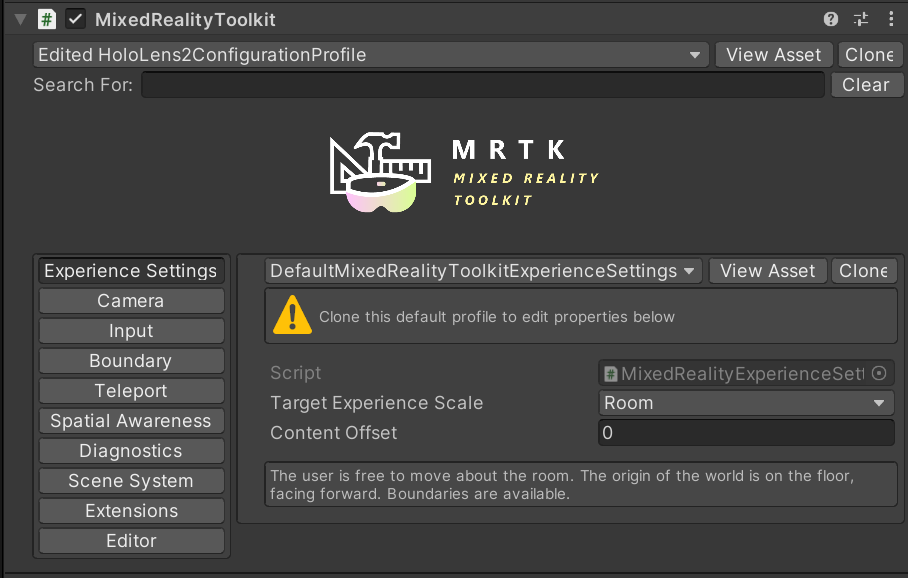
\includegraphics[width=\textwidth]{images/MRTK-profiles.png}
    \caption{Profili MRTK.}
    \label{fig:figure25}
\end{figure}

In questo caso sono state abilitate le funzionalità dei profili Spatial Awareness e Boundary System ed è stata occlusa la vista della mesh. In questo modo durante la sessione di utilizzo HoloLens 2 si occupa di mappare l'ambiente senza che l'utente se ne renda conto.

Per il posizionamento degli oggetti della scena sono stati importati in Unity il pacchetto TextMeshPro e il pacchetto \href{https://github.com/microsoft/MixedRealityLearning/releases/tag/getting-started-v2.5.0}{Tutorial Assets} di Microsoft, che offre diversi asset, utili per lo svluppo.

\subsection{Funzionamento dell'Applicazione}
Una volta importati i package correttamente è possibile aggiungere gli oggetti nella scena (Figura \ref{fig:figure26}).
In questa applicazione sono stati aggiunti:
\begin{itemize}
    \item Un cubo (\textbf{A1}) ancorato alla mesh e un modello del Rover Curiosity (\textbf{A2}) della NASA come figlio.
    \item Un cubo (\textbf{B1}) disposto su un piano (\textbf{B2}), al quale viene applicata la forza di gravità.
    \item Un cubo (\textbf{C1}) non ancorato alla mesh con una sfera (\textbf{C2}) come figlio che gli ruota attorno.
\end{itemize}

\begin{figure}[t]
    \centering
    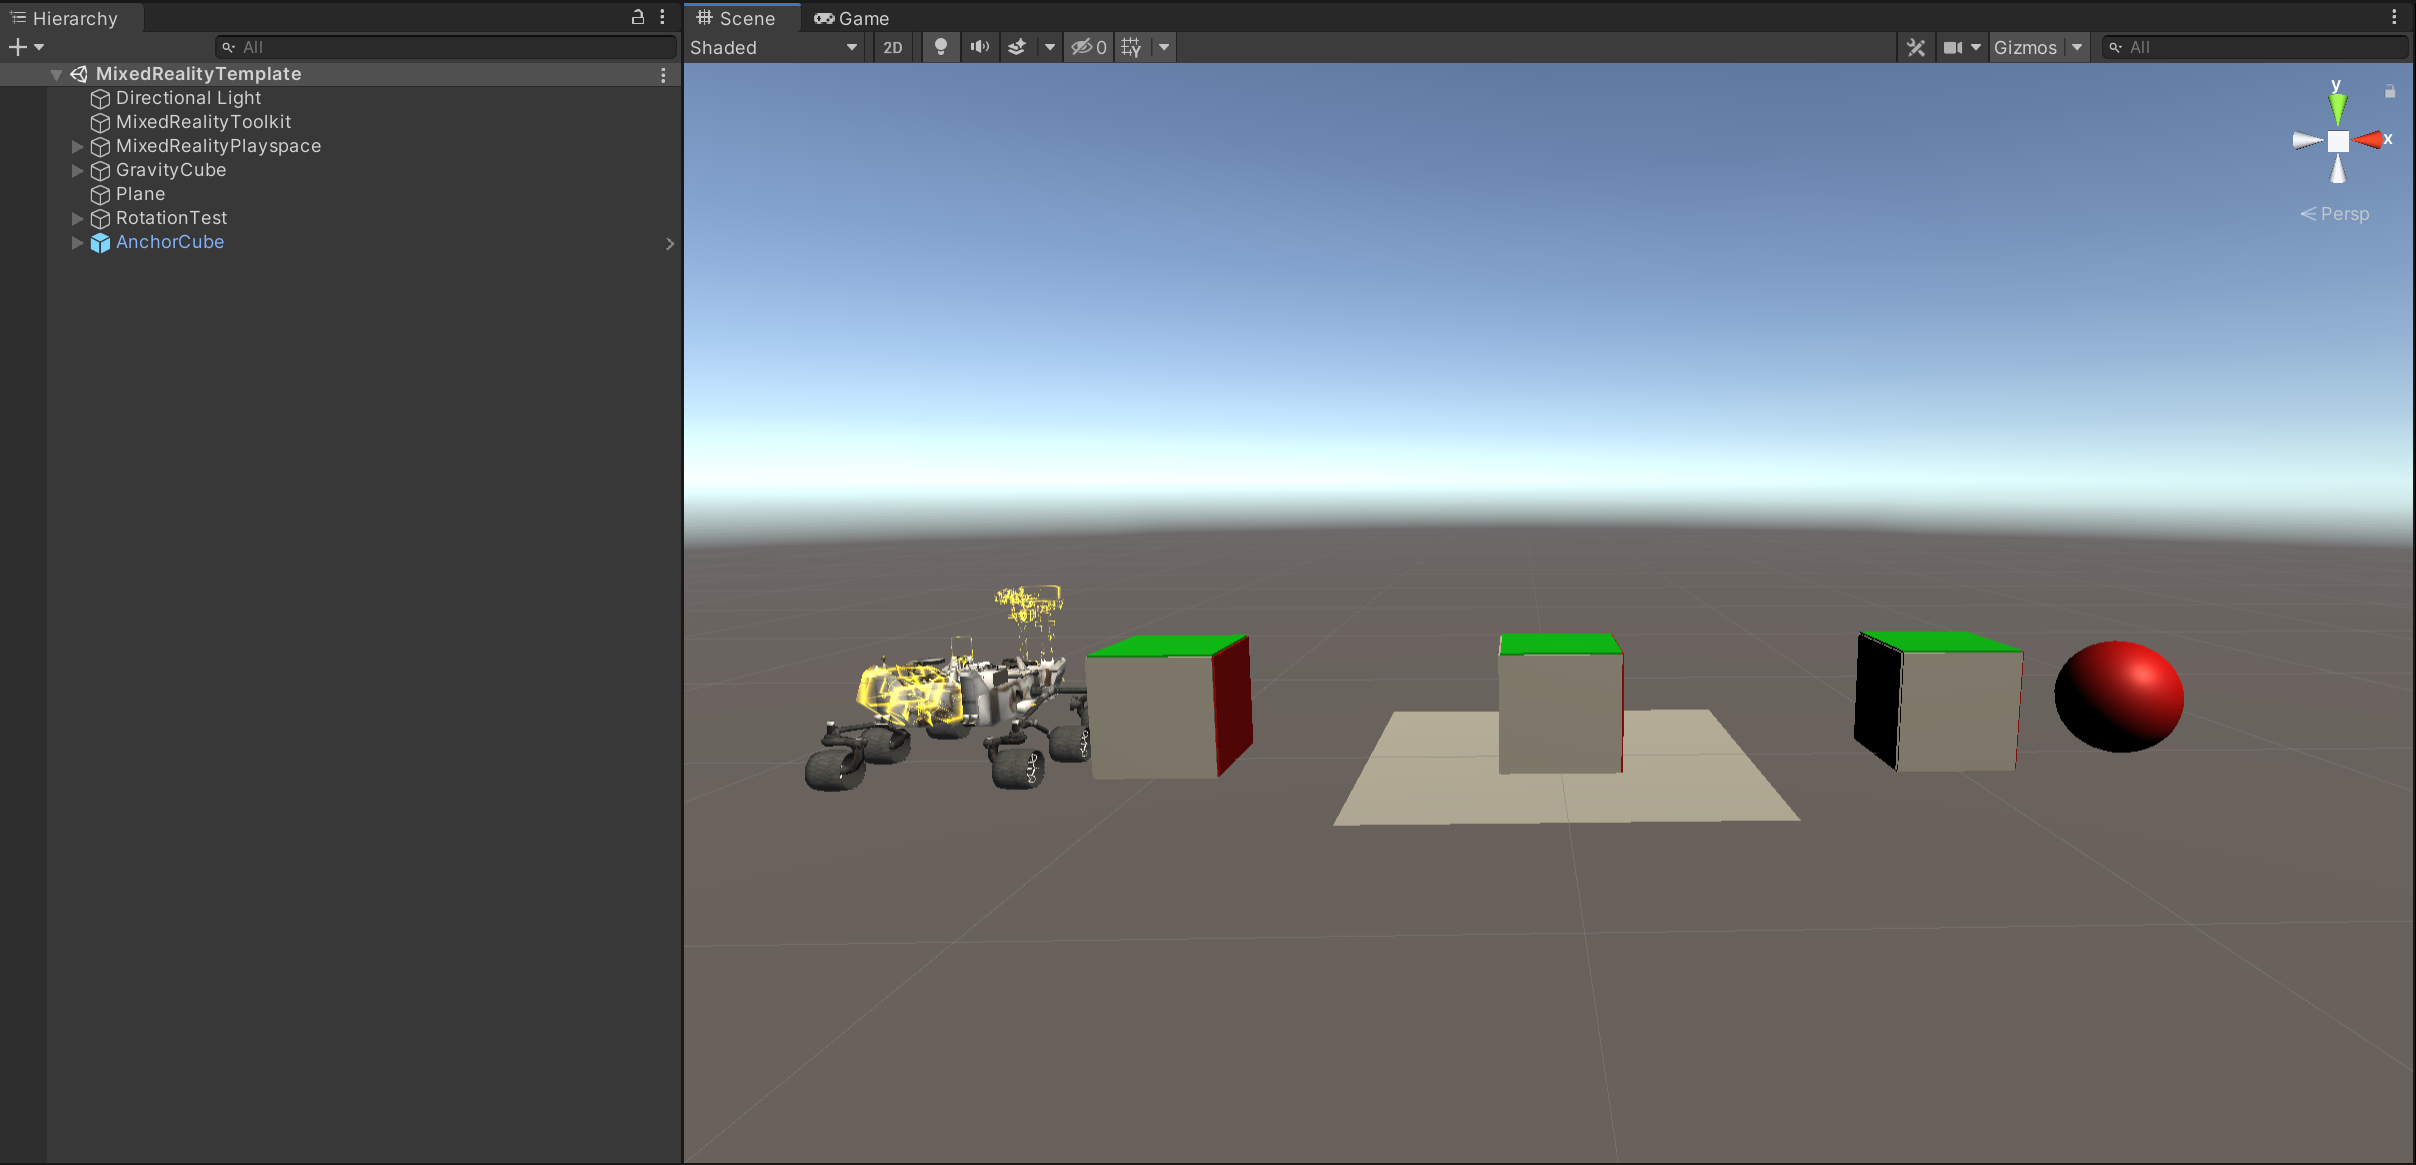
\includegraphics[width=\textwidth]{images/unity-scene.png}
    \caption{Scena di Unity.}
    \label{fig:figure26}
\end{figure}

Per abilitare la manipolazione degli ologrammi vengono aggiunti gli script Object Manipulator e NearInteractionGrabbable a tutti gli oggetti della scena, tranne che al piano \textbf{B2}. Questi due script fanno parte dei componenti del MRTK.
Object Manipulator permette di manipolare un ologramma sfruttando il gaze, così è possibile interagire con gli ologrammi anche se sono distanti. NearInteractionGrabbable abilita le interazioni da vicino, permettendo di manipolare gli ologrammi prendendoli come se fossero oggetti reali.

Sfruttando il Boundary System e il componente Spatial Mapping Collider applicato al cubo \textbf{B1} è possibile abilitare le collisioni con la mesh. Per applicare la forza di gravità è stato anche aggiunto il componente Rigid Body.
Il risultato è che nel momento in cui l'utente prende \textbf{B1}, spostandolo dal piano \textbf{B2} e lasciandolo cadere a terra, \textbf{B1} colliderà con la mesh generata da HoloLens 2, ovvero con il pavimento.
Senza la presenza della mesh \textbf{B1} oltrepasserebbe il pavimento e scomparirebbe dalla scena.

In Unity, impostando l'oggetto \textbf{C2} come figlio dell'oggetto \textbf{C1}, le coordinate di \textbf{C2} saranno stabilite sulla base di quelle di \textbf{C1}. Durante l'utilizzo dell'applicazione, spostando \textbf{C1}, \textbf{C2} si muoverà di conseguenza mantenendo la rotazione attorno a \textbf{C1}, non vale il contrario.

Per quanto riguarda la gestione delle ancore è stato sfruttato il World Anchor Store, una funzionalità del MRTK che permette di salvare la posizione di un ologramma all'interno di un ambiente (su un solo dispositivo).
È stata associata un'ancora al cubo \textbf{A1}, che viene eliminata nel momento in cui l'utente interagisce con l'ologramma e ricreata al termine dell'interazione.
L'ancora viene salvata nel World Anchor Store, che si occupa di renderla persistente e disponibile attraverso diverse sessioni.
La posizione di \textbf{A2} è comunque sempre relativa a quella di \textbf{A1}; quindi, attraverso sessioni differenti, \textbf{A1} manterrà posizione e rotazione, mentre \textbf{A2} assumerà posizione e rotazione stabilite in Unity relativamente ad \textbf{A1}. 

Per la gestione delle ancore è stato sviluppato uno script che una volta associato a un oggetto permette di salvare (listato \ref{lst:listato3}) ed eliminare (listato \ref{lst:listato2}) l'ancora associata.

\lstset{language=[Sharp]C, numbers=left}
\begin{lstlisting}[caption={Metodo richiamato per eliminare l'ancora dell'ologramma associato.}, label=lst:listato2]
    public void DeleteExistingAnchor()
    {
        WorldAnchor anchor = rootGameObject.GetComponent<WorldAnchor>();
        if (anchor != null)
        {
            Destroy(anchor);
            worldAnchorStore.Delete(rootGameObject.name);
            this.savedRoot = false;
        }
    }
\end{lstlisting}

\begin{lstlisting}[caption={Metodo richiamato per salvare l'ancora dell'ologramma associato.}, label=lst:listato3]
    public void SaveAnchor()
    {
        WorldAnchor anchor = rootGameObject.AddComponent<WorldAnchor>();
        if (!this.savedRoot && anchor != null)
        {
            this.savedRoot = this.worldAnchorStore.Save(rootGameObject.name, anchor);
        }
    }
\end{lstlisting}

Per ogni sessione, prima di utilizzare le ancore del World Anchor Store è necessario richiedere il caricamento in modo asincrono di quest'ultimo (listato \ref{lst:listato1}). Una volta caricato il World Anchor Store è possibile caricare le ancore salvate nelle sessioni precedenti (listato \ref{lst:listato4}).

\begin{lstlisting}[caption={Metodo richiamato una volta caricato il World Anchor Store.}, label=lst:listato1]
    void Start()
    {
        WorldAnchorStore.GetAsync(StoreLoaded);
    }

    private void StoreLoaded(WorldAnchorStore store)
    {
        worldAnchorStore = store;
        LoadAnchor();
    }
\end{lstlisting}

\begin{lstlisting}[caption={Metodo richiamato per reperire l'ancora dal World Anchor Store.}, label=lst:listato4]
    private void LoadAnchor()
    {
        this.savedRoot = this.worldAnchorStore.Load(rootGameObject.name, rootGameObject);
    }
\end{lstlisting}
\chapter{Esempi di Applicazioni per Hololens 2}\label{chap:capitolo3}

I possibili settori di applicazione di HoloLens 2 sono svariati. In generale, in qualsiasi ambiente la realtà mista può essere introdotta per aumentare produttività, efficienza e sicurezza.

Di seguito vengono riportati alcuni ambiti in cui l'introduzione di HoloLens 2 ha giocato un ruolo fondamentale per quanto riguarda gli aspetti appena descritti.

\section{Ambito Industriale}\label{sec:Sezione3.1}
Per quanto riguarda l'ambito industriale si può fare riferimento ai partner Microsoft, come Airbus.
Airbus è un pioniere nella tecnologia aerospaziale e leader nella progettazione e produzione di aerei commerciali e militari, satelliti e veicoli di lancio, si è impegnata a trasformare i processi industriali tradizionali attraverso l'uso della realtà mista. L'azienda ha stretto una partnership con Microsoft per utilizzare la realtà mista di Azure e HoloLens 2 come mezzo per accelerare la progettazione e la produzione di aeromobili, aumentando al contempo la sicurezza e la funzionalità e garantendo opportunità di sviluppo professionale per i dipendenti. Servizi intelligenti come Azure Remote Rendering stanno cambiando il modo in cui vengono comunicate le idee complesse. La capacità di creare applicazioni multiutente con riconoscimento dello spazio con Azure Spatial Anchors promuove una maggiore collaborazione aumentando la qualità, la sicurezza e la protezione. Airbus sta usando la realtà mista di Azure per sbloccare tutto il potenziale di HoloLens 2 e, di conseguenza, prevede di ridurre i tempi di convalida del progetto dell'80\% e di accelerare le attività complesse durante l'assemblaggio del 30\%.

Airbus ha impiegato 40 anni per costruire i suoi primi 10.000 velivoli. Nei prossimi 20 anni, il gigante aerospaziale mira a costruirne altri 20.000, una sfida formidabile che richiederà innovazioni all'avanguardia.

Jean-Brice Dumont, Executive Vice President of Engineering di Airbus, afferma:

\begin{center}
    “La nostra sfida nei prossimi anni è quella di produrre più velivoli più velocemente, e per questo dobbiamo consentire ai nostri lavoratori di essere molto meglio equipaggiati e di essere molto più efficaci in quello che fanno. Dobbiamo alzare il tiro.
    Per affrontare questa sfida, intendiamo fare un uso intenso della realtà mista ed è per questo che abbiamo stretto una partnership con Microsoft.
    La realtà mista può aiutarci ad aumentare la qualità, la sicurezza e la protezione. Il livello di errore umano è significativamente ridotto e, nel settore aerospaziale, una maggiore qualità è una maggiore sicurezza".
\end{center}

La tecnologia Microsoft Mixed Reality può essere utilizzata per aiutare gli addetti alla produzione di Airbus ad accedere a informazioni e istruzioni mentre hanno le mani occupate, ad esempio. Può anche facilitare la formazione senza impegnare attrezzature costose o persino richiedere al tirocinante di recarsi nel luogo in cui si trova l'attrezzatura. Questo è solo l'inizio: Airbus ha identificato più di 300 casi d'uso per la realtà mista.

Airbus ha ottenuto risultati impressionanti nelle sue prove e implementazioni della tecnologia di realtà mista Microsoft nella formazione, nella progettazione e nella produzione.

La realtà mista consente ai tirocinanti aerospaziali di apprendere in un ambiente virtuale immersivo senza la necessità di un vero aereo fisico o di parti. Questo ambiente 3D può offrire funzionalità che l'allenamento nella vita reale non può offrire, come la possibilità di visualizzare gli elementi in tre dimensioni da qualsiasi angolazione.

HoloLens aiuta i progettisti di Airbus a testare virtualmente i loro progetti per vedere se sono pronti per la produzione. La realtà mista accelera notevolmente il processo, riducendo il tempo impiegato dell'80\%.

La tecnologia della realtà mista può anche aiutare i lavoratori della linea di produzione ad accedere a informazioni cruciali mantenendo le mani libere. Le informazioni digitali, come istruzioni o diagrammi, possono essere sovrapposte a un vero macchinario per aiutare in attività complesse o difficili. Questi tipi di soluzioni di realtà mista hanno consentito ad Airbus di ridurre di un terzo i tempi di produzione migliorando al contempo la qualità.

\section{Ambito Sanitario}\label{sec:Sezione3.2}
In ambito sanitario sono stati prodotti vari articoli scientifici che, grazie ad HoloLens, propongono soluzioni per migliorare la precisione e l'efficienza delle operazioni e per ridurre l'esposizione degli operatori alle radiazioni.

La tecnologia olografica di HoloLens 2 può essere utile per interventi guidati da CT \footnote{La tomografia computerizzata (in inglese computed tomography) è un processo che visualizza le informazioni anatomiche da un piano di sezione trasversale del corpo.} rendendoli più sicuri ed efficienti.
In questo articolo \cite{Augmented-Reality-Assisted-CT-Guided-Interventions} È stato eseguito uno studio prospettico per valutare il direzionamento dell'ago guidato da CT su un fantoccio addominale (Figura \ref{fig:figure3a}) con e senza guida AR (rispettivamente Figura \ref{fig:figure3d} e Figura \ref{fig:figure3c}). 
L'allineamento è stato eseguito automaticamente su una griglia TC utilizzata di routine nella pratica clinica, invece di utilizzare marker esterni basati su immagini, richiesti invece in altri sistemi.

Hanno partecipato in totale otto operatori con diversa esperienza clinica che hanno eseguito un totale di 86 passaggi con ago. L'efficienza della procedura, la dose di radiazioni e i tassi di complicanze sono stati confrontati con e senza guida AR.

In Figura \ref{fig:figure3d} l'allineamento con il mondo reale appare accurato, le linee della griglia CT reali sono allineate con le linee della griglia virtuale. L'ago è allineato con la guida virtuale (linea viola) che mostra la traiettoria ideale verso la lesione selezionata (pallina verde).

\begin{figure}[t]
    \centering
    \begin{subfigure}{0.45\textwidth}
        \centering
        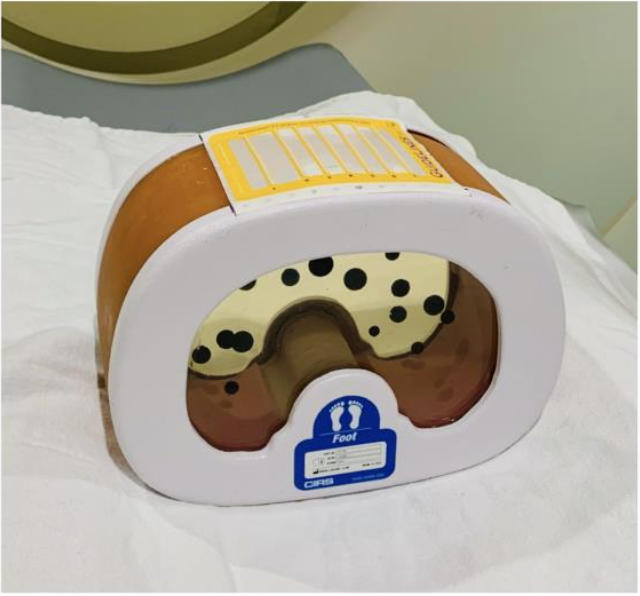
\includegraphics[width=\textwidth]{images/phantom.png}
        \caption{Griglia CT applicata alla superficie del modello.}
        \label{fig:figure3a}
    \end{subfigure}
    \begin{subfigure}{0.45\textwidth}
        \centering
        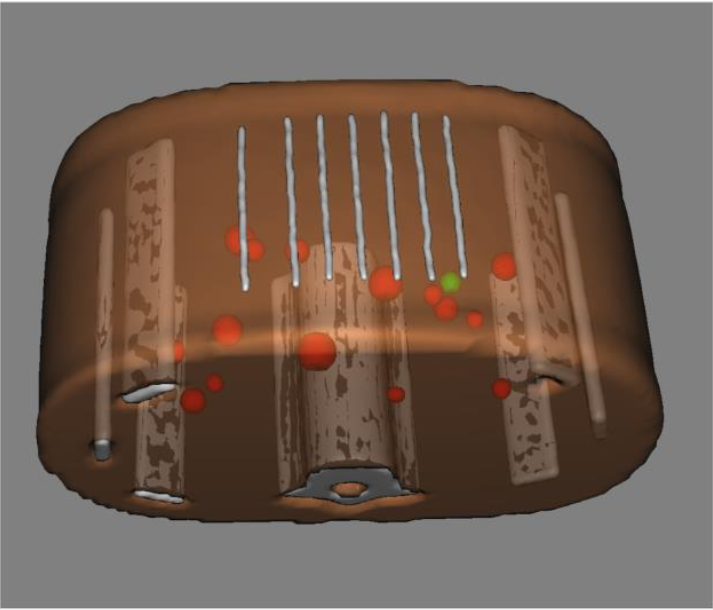
\includegraphics[width=\textwidth]{images/phantom-3D-model.png}
        \caption{Modello 3D del fantoccio.}
        \label{fig:figure3b}
    \end{subfigure}
    \begin{subfigure}{0.45\textwidth}
        \centering
        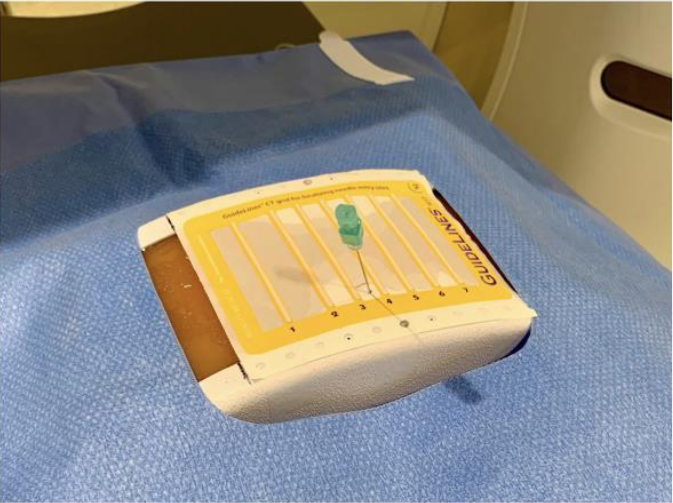
\includegraphics[width=\textwidth]{images/phantom-target.png}
        \caption{Inserimento dell'ago senza AR.}
        \label{fig:figure3c}
    \end{subfigure}
    \begin{subfigure}{0.45\textwidth}
        \centering
        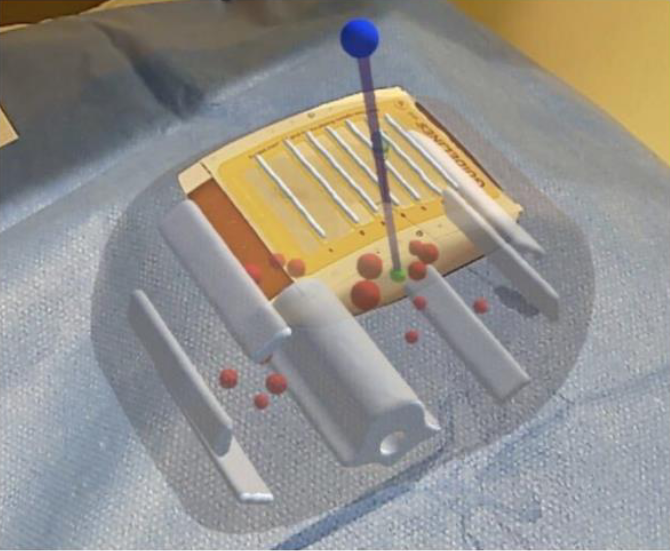
\includegraphics[width=\textwidth]{images/phantom-ologram.png}
        \caption{Inserimento dell'ago con modello tridimensionale e guida dell'ago virtuale proiettati sul fantoccio tramite HoloLens 2.}
        \label{fig:figure3d}
    \end{subfigure}
       \label{fig:figure3}
\end{figure}

Il numero medio totale di passaggi per raggiungere l'obiettivo è stato ridotto da 7,4 passaggi senza AR a 3,4 passaggi con AR (riduzione del 54,2\%).
Il tasso di errore, introdotto nel colpire una lesione non mirata è diminuito dall'11,9\% senza AR (7/59 passaggi con ago) allo 0\% con AR (0/27 passaggi con ago). I passaggi con AR erano più allineati con la traiettoria ideale del bersaglio rispetto a quelli senza AR (offset rispettivamente di 4,6° e 8,0°).

La guida 3D AR può fornire miglioramenti significativi nell'efficienza procedurale e nel risparmio della dose di radiazioni per individuare lesioni difficili e fuori dal piano. La guida AR ha elevato le prestazioni di tutti gli operatori allo stesso livello indipendentemente dalla precedente esperienza clinica.
I risultati chiave dei test effettuati sono i seguenti:
\begin{itemize}
    \item I passaggi totali con ago e la dose di radiazioni sono significativamente ridotti utilizzando la realtà aumentata.
    \item Il tasso di errore, introdotto nel colpire una lesione non mirata viene eliminato utilizzando la realtà aumentata.
    \item La realtà aumentata ha elevato le prestazioni di tutti gli operatori allo stesso livello indipendentemente dalla precedente esperienza clinica.
\end{itemize}

\section{Ambito Educativo}\label{sec:Sezione3.3}

Negli ultimi anni, il settore dell'istruzione ha incorporato nelle classi l'uso di nuove tecnologie e dispositivi informatici, che hanno consentito di implementare nuovi modi per migliorare l'insegnamento e l'apprendimento. La realtà aumentata può essere impiegata per aiutare gli insegnanti a promuovere l'interesse degli studenti nell'apprendimento di determinate materie e concetti astratti in nuove modalità visive. Questo articolo \cite{Augmented-Reality-Teaching-System} propone di sfruttare il potenziale di HoloLens al fine di integrare esperienze AR nelle lezioni e nei laboratori pratici. Nello specifico, viene proposta un'architettura per fornire servizi didattici AR a bassa latenza in un'aula o in un laboratorio. Una latenza così bassa è ottenuta grazie all'uso di dispositivi di edge computing, che esonerano il cloud dalle attività tradizionali richieste dalle applicazioni AR dinamiche (ad esempio, elaborazione dei dati in tempo reale, comunicazioni tra dispositivi AR). A seconda dell'applicazione AR specifica e del numero di utenti, il collegamento wireless (di solito WiFi) potrebbe essere sovraccaricato se la rete non è stata progettata correttamente e le prestazioni complessive dell'applicazione possono essere compromesse, portando a un'elevata latenza e persino a problemi di comunicazione. Per affrontare questo problema, le misurazioni del canale radio e i risultati della simulazione sono stati eseguiti per mezzo di uno strumento di ray-launching 3D sviluppato internamente, che è in grado di modellare e simulare il comportamento di un'aula/laboratorio abilitato per AR in termini di propagazione radio e qualità del servizio.

La Figura \ref{fig:figure32} illustra l'architettura di comunicazione del sistema proposto. In fondo è presente il livello AR-IoT, che è diviso in due sottolivelli: il sottolivello dei dispositivi AR, che è composto dai dispositivi AR utilizzati dagli studenti e dall'insegnante, e il sottolivello dei dispositivi IoT (ovvero, oggetti smart come sensori e attuatori) che sono presenti nell'ambiente. Entrambi i dispositivi AR e IoT sono collegati tramite un punto di accesso WiFi (AP) o un gateway al livello di edge computing, dove vengono eseguiti i servizi educativi AR. Nello specifico, lo strato edge computing è conformato da due sottolivelli:

\begin{itemize}
    \item \textbf{AR Service Sublayer}: utilizza dispositivi di edge computing come cloudlet \footnote{È un data center cloud su piccola scala ottimizzato per la mobilità che si trova ai "margini" di Internet.} o fog di gateway \footnote{È un'architettura che utilizza dispositivi periferici per eseguire una notevole quantità di calcolo, archiviazione e comunicazione localmente per poi instradarla su Internet.} basati su single board computer (SBC) \footnote{È un computer completo costruito su un unico circuito, con microprocessore, memoria, input/output e altre caratteristiche richieste da un computer. } per fornire risposte veloci e distribuite. Gli insegnanti possono agire come amministratori locali dei dispositivi su questo livello per controllare quali contenuti vengono mandati ai dispositivi AR degli studenti. Inoltre, i dispositivi di edge computing di questo livello consentono la condivisione di esperienze AR, potendo così sincronizzare il contenuto condiviso contemporaneamente tra più utenti.
    \item \textbf{AR-IoT Service Sublayer}: consente di interconnettere dispositivi AR e IoT senza soluzione di continuità. Il sistema presentato utilizza Message Queue Telemetry Transport (MQTT) \footnote{È un protocollo di rete leggero di tipo publish-subscribe, che trasporta i messaggi tra i dispositivi. } e un'API (Application Programming Interface) REpresentational State Transfer (REST) per facilitare gli scambi di dati tra più dispositivi eterogenei. Per quanto riguarda il servizio AR-IoT Bridge, si tratta di un componente software che collega le richieste MQTT e API REST, avvalendosi di determinati servizi ausiliari quando necessario.
\end{itemize}

\begin{figure}[t]
    \centering
    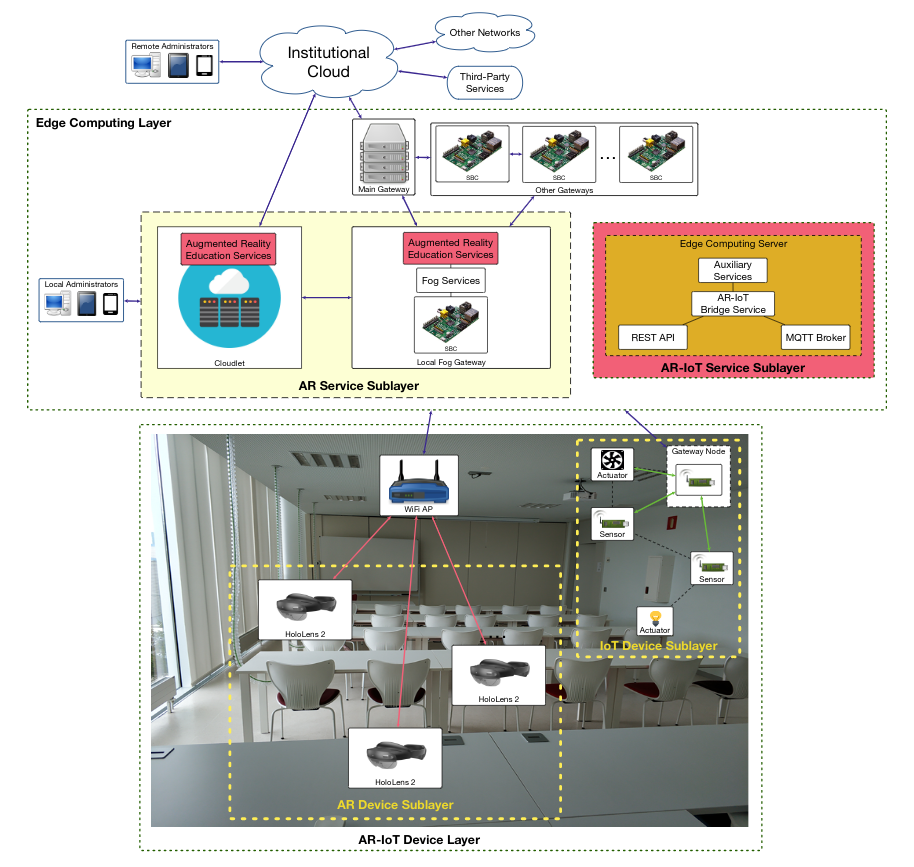
\includegraphics[width=\textwidth]{images/Communications-architecture.png}
    \caption{Architettura di comunicazione del sistema proposto.}
    \label{fig:figure32}
\end{figure}

Entrambi i livelli consentono di implementare le funzionalità più avanzate del sistema:

\begin{itemize}
    \item L'insegnante è in grado di controllare da remoto quando e come il contenuto AR viene visualizzato sui visori HoloLens 2 utilizzati dagli studenti.
    \item Gli studenti possono condividere la stessa esperienza AR e quindi collaborare tra loro per raggiungere un obiettivo comune.
    \item Il sistema sviluppato può interagire con gli oggetti IoT circostanti, consentendo agli utenti AR di ottenere informazioni o di agire con essi.
    \item Poiché l'applicazione HoloLens 2 rileva le azioni eseguite da ogni studente, è possibile registrarle e quindi determinare le prestazioni dello studente o i suoi contributi durante le attività di collaborazione.
\end{itemize}

\section{Ambito Museale}\label{sec:Sezione3.4}
Un altro ambito di applicazione interessante è quello del museo.
Infatti è possibile sviluppare applicazioni AR utili per guidare l'utente all'interno del museo.
Entrando più nello specifico, si può proporre una guida virtuale che, oltre a guidare l'utente, permetta di interagire con i modelli 3D relativi agli artefatti presenti all'interno del museo.
Una soluzione del genere viene proposta in questo articolo \cite{HoloLens-in-museum}, dove è stata utilizzata la prima versione di HoloLens.
Questa procedura mira a creare un quadro di orientamento semplice, interattivo e informativo da utilizzare per gli utenti dei musei. L'applicazione MR richiede all'utente di indossare Microsoft HoloLens ed esplorare una serie di contenuti virtuali attraverso l'interfaccia utente. Un ambiente popolato da reperti museali è necessario per sovrapporre virtualizzazioni digitali e informazioni affinché il sistema di guida virtuale del tour possa funzionare. 
L'applicazione proposta (Figura \ref{fig:figure33}) fornisce le seguenti funzionalità:
\begin{itemize}
    \item Controllo degli ologrammi relativi ai manufatti museali, con possibilità di ruotarli di 360 gradi.
    \item Pulsanti che avviano testo e immagini per permettere all'utente di ricevere informazioni.
    \item Interazione con il sistema di guida virtuale, che presenta informazioni audio e video in tempo reale.
    \item Utilizzo di piccoli cerchi che funzionano come oggetti trigger per rivelare informazioni su particolari aree di interesse.
\end{itemize}

\begin{figure}[t]
    \centering
    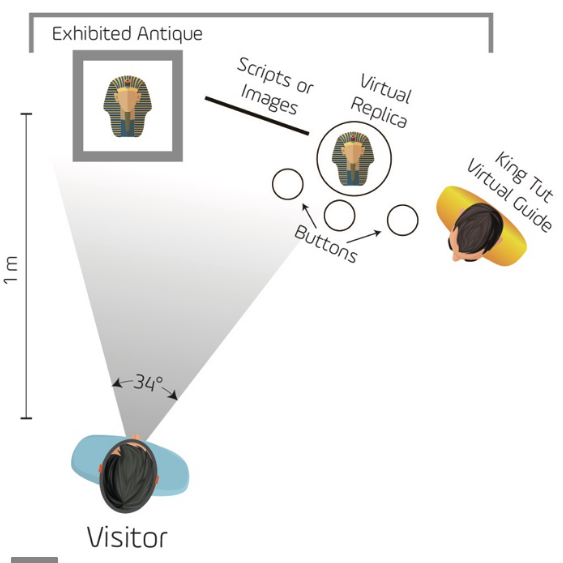
\includegraphics[width=0.6\textwidth]{images/museum.png}
    \caption{Scena di esempio dell'applicazione.}
    \label{fig:figure33}
\end{figure}

Nell'articolo vengono presentati i risultati dei test eseguiti su un campione di utenti.
Il campione di popolazione valutato includeva nove esperti in diverse discipline accademiche che vanno dall'interazione uomo-macchina (in inglese human-computer interaction, HCI) alla comunicazione visiva. Considerando gli esperti di HCI e di comunicazione visiva in questa valutazione è stata presa in considerazione la loro capacità di valutare l'usabilità, l'interattività e il livello di esperienza utente acquisita. Quindi, gli esperti di studi museali sono stati considerati per valutare se questo sistema può raggiungere ciò che i visitatori richiedono nei musei e per strutturarlo in base alla natura delle visite. Considerare gli esperti per questa valutazione ha un doppio vantaggio: come menzionato hanno esperienza e possono anche essere generalmente visitatori di musei, quindi le loro risposte possono essere più critiche e vantaggiose per lo studio rispetto a quelle  dei normali visitatori del museo.

Il prototipo dell'applicazione ha ottenuto risultati complessivamente positivi sia in termini di usabilità che di accessibilità.
\chapter{Caso di Studio}

\section{Descrizione del Caso di Studio}

Come detto nel capitolo \ref{chap:capitolo3}, l'applicazione della realtà mista in determinati settori può incrementare notevolmente efficienza, produttività e sicurezza.
Grazie alla realtà mista, è possibile creare esperienze in cui gli utenti possono interagire fra loro e con l'ambiente in nuovi modi.
Queste nuove interazioni possono essere introdotte digitalizzando le entità reali e le informazioni presenti nell'ambiente.
Avere una rappresentazione digitale di un dispositivo può permettere di osservarne lo stato e di controllarlo senza dover interagire direttamente con quel dispositivo. Per quanto riguarda le informazioni, è possibile avere rappresentazioni che evidenziano determinati aspetti, utili al tipo di utente che sta eccedendo a quell'informazione.
In un ambiente MR più utenti possono anche interagire contemporaneamente con la stessa informazione sfruttando rappresentazioni differenti.
È anche possibile condividere la stessa rappresentazione di un dispositivo o di un'informazione con più utenti contemporaneamente, in modo da permettere esperienze condivise in tempo reale.
Le rappresentazioni digitali possono essere generate - grazie a determinate tecniche di riconoscimento - semplicemente osservando le informazioni o gli oggetti presenti nell'ambiente.

Dal punto di vista della condivisione, le informazioni e le loro rappresentazioni possono essere condivise fra più utenti secondo le seguenti modalità:
\begin{itemize}
    \item Vengono condivise rappresentazioni differenti della stessa informazione. In questo modo diversi utenti possono accedere alle stesse informazioni contemporaneamente, ma in luoghi e con modalità differenti.
    \item Viene condivisa la stessa rappresentazione dell'informazione fra più utenti, quindi in allineamento sia spaziale che temporale, così da permettere esperienze condivise e collaborazioni in uno stesso ambiente.
\end{itemize}

Considerando entrambi i punti, un singolo utente può visualizzare contemporaneamente sia rappresentazioni condivise con altri utenti che locali.

Le rappresentazioni presenti nell'ambiente devono comportarsi come se fossero oggetti reali, quindi devono essere considerate come entità attive.
Per quanto riguarda le rappresentazioni relative ai dispositivi presenti nell'ambiente, un'azione su una rappresentazione produce un cambiamento di stato sul dispositivo associato.
Allo stesso modo, se avviene un cambiamento di stato su un dispositivo, le sue rappresentazioni devono essere aggiornate.

Un'applicazione MR con le caratteristiche appena descritte può essere introdotta in vari ambiti, fra cui quelli presentati nel capitolo \ref{chap:capitolo3}.
Tuttavia, in questo caso di studio si vuole considerare in particolar modo il settore sanitario, nel quale la realtà mista può essere utilizzata per migliorare le collaborazioni fra medici e infermieri o per controllare in modo più efficiente l'ambiente in determinate situazioni, per esempio nel momento in cui si effettuano operazioni.

Uno dei possibili casi di utilizzo può essere l'analisi di determinati documenti o referti, contenenti informazioni che possono essere visualizzate secondo punti di vista differenti, anche in base al tipo di utente che le sta osservando. 

Un esempio può essere l'analisi dei risultati di una TAC presente su un computer: il medico deve poter "prendere" le informazioni e portarle nell'ambiente, rendendole indipendenti dal dispositivo in cui risiedono. Nell'esempio della TAC può essere creato un modello 3D che permetta un'analisi più dettagliata rispetto a una serie di immagini.
Inoltre, medici e infermieri devono avere la possibilità di visualizzare solo i dati della TAC interessati.

L'obiettivo del caso di studio è proprio quello di realizzare un'applicazione MR per HoloLens 2 che possa essere impiegata in ambito sanitario.

Un operatore deve essere in grado di aggiungere facilmente nuove informazioni e di poterle condividere con altri operatori, quindi sorge la necessità di rendere l'informazione indipendente dal dispositivo che si utilizza. Inoltre ogni informazione deve essere identificata in modo univoco, in modo da evitare fraintendimenti.
Nell'ambiente di realtà mista possono quindi essere presenti contemporaneamente informazioni private (relative a un solo dispositivo) e condivise, in tutto o in parte.

Oltre alle informazioni devono essere identificati correttamente gli oggetti e i dispositivi dei quali si vuole gestire una rappresentazione.

Inoltre, bisogna stabilire delle politiche di accesso in lettura e scrittura sia per i dispositivi che per le informazioni.
Ogni operatore ha quindi determinati diritti di accesso sulle rappresentazioni che può utilizzare.

\section{Analisi dei Requisiti}

Uno degli aspetti chiave nella realizzazione del sistema è la necessità di dover "informare" HoloLens su ciò che si sta guardando, in modo così che possa proiettare e condividere le rappresentazioni adeguate.
HoloLens deve poter rilevare informazioni (come risonanze, TAC e radiografie) e gli oggetti di cui si vuole gestire una rappresentazione. Una delle soluzioni più adatte per realizzare questa funzionalità è l'utilizzo di marker.
A ogni informazione e dispositivo deve essere associato un marker che possa essere rilevato correttamente da HoloLens. Nello specifico è possibile realizzare un marker ad hoc per ogni informazione o utilizzare l'informazione vera e propria come marker.

Per virtualizzare determinati tipi di informazioni non è possibile sfruttare immagini 2D, quindi sorge la necessità di rilevare oggetti 3D, per esempio un monitor multi-parametrico relativo a un paziente. Nel caso specifico, una volta riconosciuto il monitor, HoloLens deve proiettare nell'ambiente una copia delle informazioni che questo presenta.

Un altro aspetto chiave riguarda la condivisione delle informazioni, che può avvenire in modalità differenti.
Per quanto riguarda l'accesso in allineamento esclusivamente temporale è necessario astrarre l'informazione dalle sue copie virtuali presenti nell'ambiente.
Invece per le esperienze condivise in cui più operatori devono collaborare e interagire con gli stessi ologrammi bisogna condividere non solo le informazioni, ma anche posizione e rotazione degli ologrammi, in modo da garantire un allineamento sia temporale che spaziale.
Per realizzare questa funzionalità si può sfruttare un servizio che permette di autenticare gli operatori e di condividere le informazioni nelle modalità descritte.

Il servizio in questione deve anche permettere l'interazione degli ologrammi con il mondo reale, in particolare con i dispositivi IoT presenti nell'ambiente.

L'utilizzo di un servizio permette anche l'accesso da dispositivi e piattaforme differenti, una caratteristica utile per sviluppi futuri.

\subsection{Casi d'Uso}
In questa sottosezione vengono presentati dei casi d'uso che descrivono alcune delle azioni che gli operatori possono effettuare sfruttando l'applicazione MR.

Nel diagramma presente in Figura \ref{fig:figure4} vengono messe in evidenza le modalità di accesso alle informazioni e di richiesta delle rappresentazioni.
Un operatore, per poter accedere a qualsiasi tipo di rappresentazione, deve prima autenticarsi. Questa procedura è necessaria per poter comprendere a quali rappresentazioni l'operatore ha il diritto di accedere e con che modalità.

Una volta effettuato l'accesso, l'operatore può accedere alle rappresentazioni sfruttando i marker. In particolare, nel momento in cui viene rilevato un marker, l'operatore deve essere in grado di decidere - tramite l'utilizzo di apposite interfacce grafiche - se richiedere la rappresentazione associata. In altre parole, la rappresentazione non deve essere presentata direttamente nel momento in cui viene rilevato il marker.

Un'altra caratteristica fondamentale presentata in Figura \ref{fig:figure4} è la gestione dei permessi. Per ogni azione che viene eseguita dall'operatore su una rappresentazione devono essere controllati di diritti di accesso.

\begin{figure}[H]
    \centering
    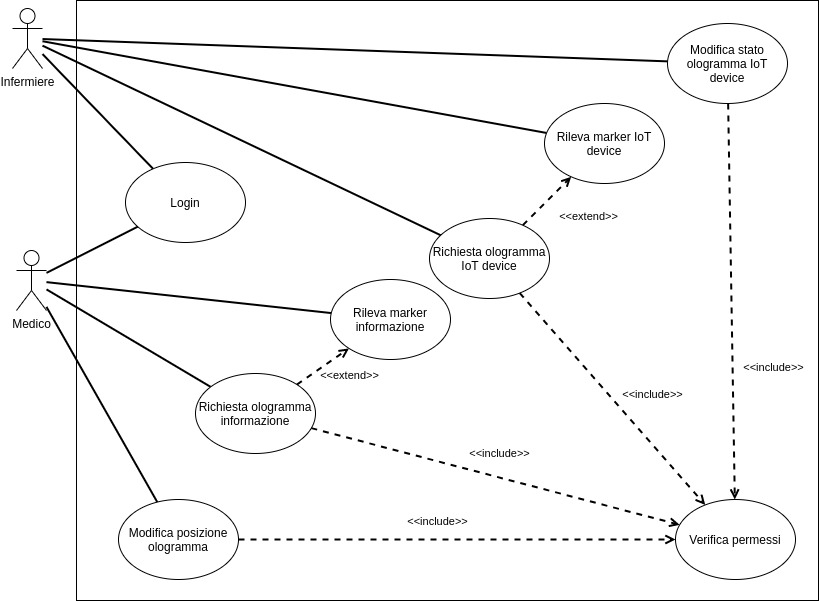
\includegraphics[width=\textwidth]{images/Casi uso-Page-1.jpg}
    \caption{Diagramma dei casi d'uso che descrive il modo in cui informazioni e dispositivi vengono digitalizzati grazie ai marker.}
    \label{fig:figure4}
\end{figure}

Nel diagramma presente in Figura \ref{fig:figure42} viene messo in evidenza il fatto che determinate azioni eseguite sulle rappresentazioni apportano modifiche sia allo stato dell'ambiente che alle altre rappresentazioni.

In questo caso abbiamo due medici che partecipano a un'esperienza condivisa, quindi condividono le stesse rappresentazioni.
Se uno dei due medici sposta, ruota o ridimensiona un ologramma, lo stesso effetto deve essere applicato all'ologramma che l'altro medico sta visualizzando.

La stessa cosa vale per i dispositivi IoT presenti nell'ambiente. Un'azione eseguita su una rappresentazione relativa a un dispositivo deve produrre un effetto sia sul dispositivo stesso che sulle sue rappresentazioni.

In Figura \ref{fig:figure42}, per alleggerire il carico grafico, vengono omessi sia il login che la verifica dei permessi per ogni azione eseguita; operazioni che devono comunque essere sempre eseguite.

\begin{figure}[H]
    \centering
    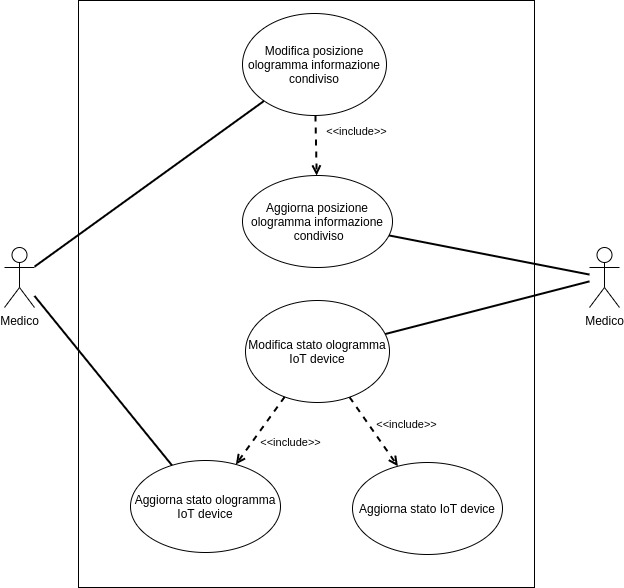
\includegraphics[width=\textwidth]{images/Casi uso-Page-2.jpg}
    \caption{Diagramma dei casi d'uso che descrive gli effetti delle interazioni con le rappresentazioni.}
    \label{fig:figure42}
\end{figure}

\subsection{Identificazione delle Informazioni e dei Dispositivi IoT nell'Ambiente}

Come detto all'inizio di questa sezione, una delle soluzioni per identificare correttamente le informazioni presenti nell'ambiente è utilizzare i marker.

Oltre ai marker deve essere realizzato un punto di condivisione - come un servizio - che si occupi di associare correttamente le rappresentazioni ai marker.
Il servizio in questione deve autenticare gli operatori e deve rendere disponibili le rappresentazioni delle informazioni e dei dispositivi IoT.

Grazie all'autenticazione dell'operatore, il servizio è in grado di gestire correttamente sia le rappresentazioni a cui è possibile accedere che i permessi relativi alle azioni che si possono eseguire sulle informazioni e sui dispositivi IoT.

È importante sottolineare che le informazioni possono avere diverse rappresentazioni, non tutte accessibili da tutti gli operatori, questo perché ogni operatore ha determinate necessità e preferisce avere rappresentazioni che evidenzino determinati aspetti dell'informazione.

In questo modo, in un ambiente MR, più utenti possono interagire con le sesse informazioni tramite rappresentazioni differenti. Ogni cambiamento di stato di un'informazione o di un dispositivo viene replicato su tutte le sue rappresentazioni grazie al servizio.

\subsection{Allineamento dei Sistemi di Coordinate}

Nelle esperienze condivise, in cui gli ologrammi devono essere presentati in allineamento spaziale e temporale, bisogna permettere la condivisione dei sistemi di coordinate fra più dispositivi.

Nello stesso ambiente, dispositivi MR possono avere sistemi di coordinate differenti. Per questo motivo, per realizzare esperienze condivise, non è possibile condividere direttamente le coordinate di un ologramma.

Bisogna stabilire dei punti di riferimento comuni all'interno dell'ambiente e condividere le coordinate degli ologrammi rispetto a quei punti.

Esprimendo le coordinate dell'ologramma rispetto a un determinato punto nell'ambiente permette di renderle indipendenti dal dispositivo che si utilizza.

Per la condivisione delle coordinate è possibile sfruttare lo stesso servizio descritto nella sottosezione precedente.

I punti di riferimento all'interno dell'ambiente possono essere stabiliti sempre sfruttando i marker, gli stessi che vengono utilizzati per riconoscere le informazioni e i dispositivi nell'ambiente.

Quindi, in un'esperienza condivisa con dispositivi differenti, nel momento in cui un operatore interagisce con un ologramma:
\begin{enumerate}
    \item Viene applicata una trasformazione alle coordinate di quell'ologramma, che vengono espresse secondo la posizione del marker associato.
    \item La posizione viene mandata al servizio.
    \item Il servizio replica le coordinate verso tutti i dispositivi che partecipano all'esperienza condivisa.
    \item In fase di ricezione ogni dispositivo converte le coordinate espresse rispetto al marker nel suo sistema di coordinate.
\end{enumerate}

\subsection{Interazioni fra Entità Virtuali e Reali}
Per quanto riguarda la realizzazione delle interazioni fra entità reali e virtuali bisogna rendere "intelligenti" le prime, introducendo quindi dispositivi IoT nell'ambiente.
Questa caratteristica può risultare utile per aumentare la capacità di controllo dell'ambiente da parte degli operatori.
Per esempio, facendo riferimento al sistema di illuminazione dell'ambiente, si potrebbe permettere di spegnere o accendere le luci in tutto o in parte da qualsiasi posizione, indipendentemente dalla posizione degli interruttori fisici.
Per realizzare questa funzionalità naturalmente bisogna registrare caratteristiche e stato di ogni dispositivo IoT e renderli disponibili per i dispositivi MR.
Bisogna anche associare correttamente il dispositivo IoT alla sua rappresentazione digitale, che deve riportarne lo stato e in determinati casi permettere di modificarlo.
Tornando all'esempio del sistema di illuminazione, è possibile gestire il suo stato tramite un ologramma che rappresenta un pannello di controllo.

Per rendere i dispositivi intelligenti si possono utilizzare sistemi integrati basati su microcontrollori o su SoC, come Arduino Uno, ESP 8266 o Raspberry Pi 4.

Per la comunicazione e l'aggiornamento dello stato dei dispositivi bisogna connettere questi ultimi alla rete e sfruttare un servizio che permetta ad HoloLens di accedere alle rappresentazioni digitali dei dispositivi intelligenti.

\section{Progettazione del Sistema}\label{sec:Sezione4.3}
Data l'analisi dei requisiti, per la realizzazione del sistema viene proposta la seguente soluzione, composta da due macro-componenti, che comunicano attraverso la rete sfruttando il protocollo HTTPS.

\begin{itemize}
    \item \textbf{Back-End Engine}: offre un insieme di servizi, grazie ai quali si occupa di autenticare gli utenti e di gestire le politiche di accesso alle informazioni e ai dispositivi intelligenti.
    \item \textbf{Holographic App}: è un'applicazione client progettatata per HoloLens, che si occupa di comunicare con il Back-End Engine per accedere alle rappresentazioni delle informazioni e dei dispositivi IoT.
\end{itemize}

In Figura \ref{fig:figure43} vengono presentati i due macro-componenti e il modo in cui comunicano, abbiamo il Back-End Engine al centro, dei dispositivi IoT e la Holographic App che sta rappresentando contemporaneamente sia ologrammi a informazioni che a dispositivi IoT.
Il Back-End Engine viene utilizzato come punto di accesso per tutti i dispositivi che fanno parte della realtà mista.
Per ogni device IoT viene espresso uno stato, che viene rappresentato dagli ologrammi associati a quel dispositivo.
I due macrosistemi interagiscono attraverso la rete nei seguenti modi:
\begin{itemize}
    \item In un'esperienza condivisa, se un operatore modifica le coordinate di un ologramma, la Holographic App invia le nuove coordinate al Back-End Engine, che le inoltra a tutti gli altri operatori.
    \item Nel momento in cui un operatore modifica un'informazione tramite una sua rappresentazione il Back-End Engine si occupa di rendere effettive e persistenti le modifiche.
    \item Se un operatore modifica lo stato di un dispositivo IoT tramite una sua rappresentazione il Back-End Engine applica effettivamente lo stato al dispositivo in questione e aggiorna tutte le sue rappresentazioni.
    \item Nel momento in cui un dispositivo IoT cambia stato (non a causa di una interazione con una sua rappresentazione) il cambiamento viene comunicato al Back-End Engine, che si occupa anche in questo caso di aggiornare tutte le sue rappresentazioni. 
\end{itemize}

\begin{figure}[H]
    \centering
    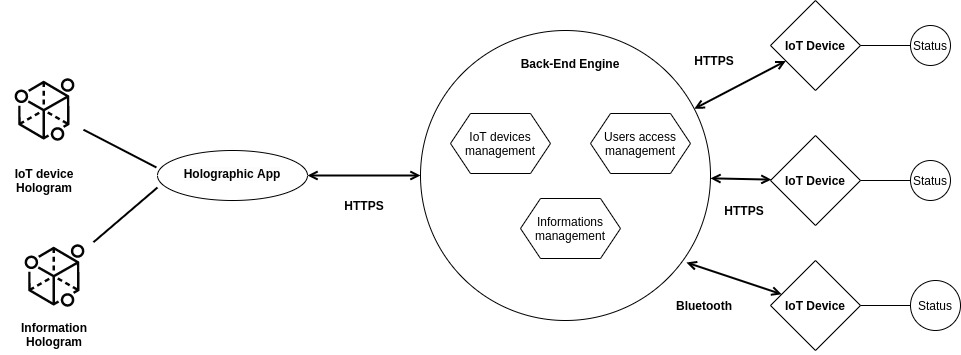
\includegraphics[width=\textwidth]{images/Diagramma-sistema.jpg}
    \caption{Diagramma che presenta il modo in cui i macro-componenti comunicano.}
    \label{fig:figure43}
\end{figure}

\subsection{Back-End Engine}
Il Back-End Engine (Figura \ref{fig:figure44}) si occupa di gestire gli utenti, le informazioni e i dispositivi IoT presenti nell'ambiente.

Questo macrosistema inoltre memorizza in modo persistente le informazioni con i relativi marker e lo stato dei dispositivi IoT presenti nell'ambiente sfruttando i componenti \texttt{IoTDeviceManager} e \texttt{InformationManager}.

Un'informazione può avere rappresentazioni distinte che coesistono allo stesso tempo. 
Fornendo questo livello di astrazione, più utenti possono interagire con le stesse informazioni in modi differenti.
Più utenti possono comunque interagire contemporaneamente con una stessa rappresentazione, condivisa in allineamento spaziale e temporale.
Uno o più utenti possono accedere a uno stesso ologramma e modificarne posizione e rotazione, che verranno replicate su tutti i dispositivi MR che stanno accedendo a quell'ologramma in quel momento; in questo modo è possibile realizzare esperienze condivise.

Le politiche di accesso, gestite dal componente \texttt{UserPolicyManager}, vengono utilizzate per permettere solo a determinati utenti di accedere alle rappresentazioni delle informazioni.
In particolare un utente, per una singola informazione, può avere accesso in lettura, in scrittura, entrambe o nessuna delle due.

I dispositivi IoT vengono suddivisi in attuatori (con possibilità di leggere e modificare lo stato) e sensori (che permettono unicamente di leggere lo stato).
Per ogni dispositivo IoT viene fornita una singola rappresentazione e un indirizzo IP.
L'accesso dai client MR verso i dispositivi IoT non è diretto, viene comunque utilizzato il servizio, perché devono essere sempre controllati i diritti di accesso.
Quindi per richiedere o modificare lo stato di un determinato dispositivo è necessario contattare il servizio.
Esattamente come per le informazioni, gli utenti hanno determinati diritti di accesso sui dispositivi IoT.

\begin{figure}[H]
    \centering
    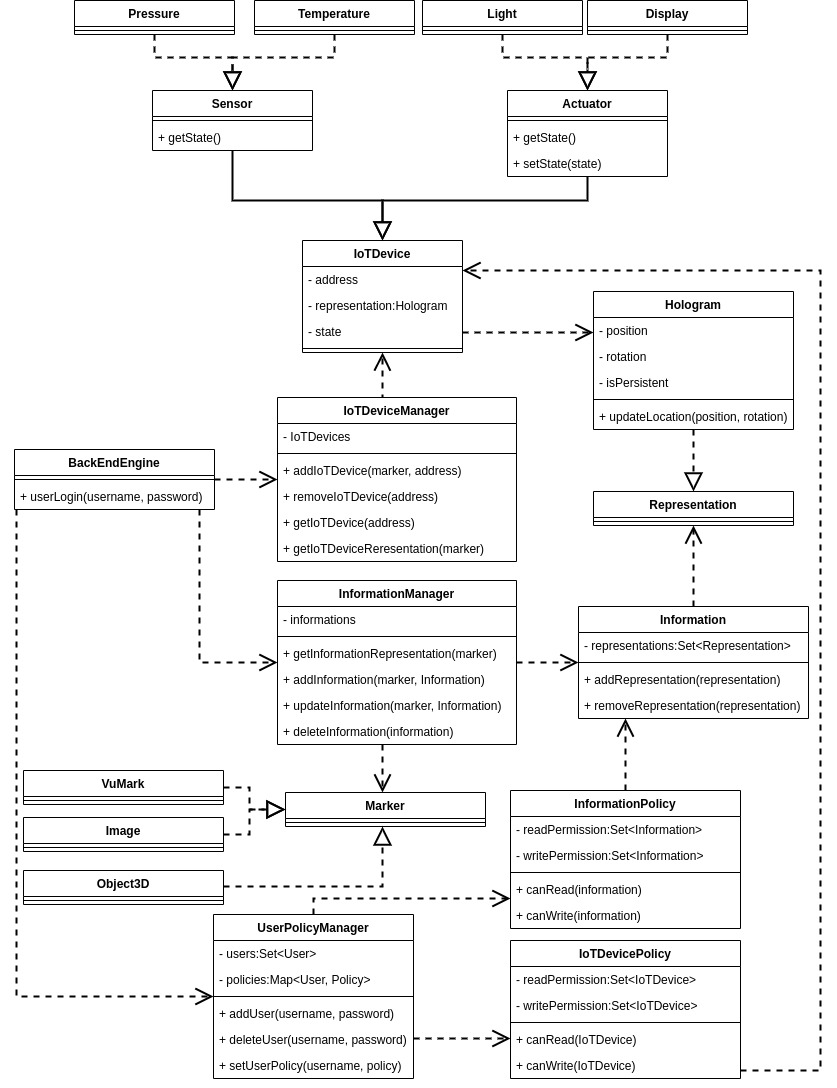
\includegraphics[width=\textwidth]{images/MR Service - Diagramma Classi.jpg}
    \caption{Back-End Engine - Diagramma delle classi.}
    \label{fig:figure44}
\end{figure}

\subsection{Holographic App}
La Holographic App (diagramma delle classi in \ref{fig:figure45}) per prima cosa si occupa sempre di richiedere le credenziali di accesso all'utente e di autenticarsi comunicando con il Back-End Engine.
Una volta eseguito l'accesso l'utente può richiedere e interagire con le rappresentazioni delle informazioni e dei dispositivi IoT presenti nell'ambiente.

Il componente \texttt{HolographicAppController} si occupa di gestire l'applicazione, comunicando con il Back-End Engine tramite \texttt{ServiceConnectionManager} e controllando gli ologrammi tramite \texttt{HologramManager}.

\texttt{ServiceConnectionManager} si occupa di comunicare con il Back-End Engine. In particolare, viene sfruttato per:
\begin{itemize}
    \item Eseguire il login.
    \item Richiedere la rappresentazione di un'informazione nel momento in cui viene rilevato un marker.
    \item Richiedere la rappresentazione di un dispositivo IoT.
    \item Spedire e ricevere le nuove coordinate di un ologramma, in modo da garantire esperienze condivise in tempo reale.
    \item Modificare lo stato di un dispositivo IoT tramite la sua rappresentazione.
\end{itemize}

In un'esperienza condivisa, se un utente modifica la posizione di un ologramma, la Holographic App manda le nuove coordinate al Back-End Engine, che si occupa di memorizzarle e di replicarle verso tutti gli altri utenti che stano partecipando a quell'esperienza.

La gestione degli ologrammi viene effettuata dall'\texttt{HologramManager}, che si occupa di istanziare e gestire le rappresentazioni delle informazioni e dei dispositivi IoT fornite dal \texttt{ServiceConnectionManager}.

\texttt{HologramManager} si occupa anche di applicare affettivamente le nuove coordinate degli ologrammi fornite dal Back-End Engine durante un'esperienza condivisa.

\begin{figure}[H]
    \centering
    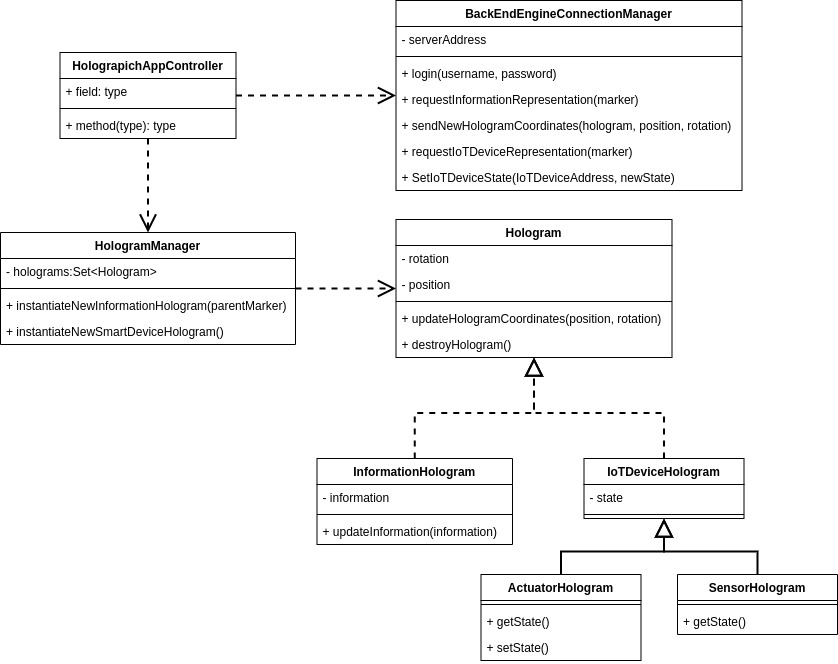
\includegraphics[width=\textwidth]{images/MR Client - Diagramma Classi.jpg}
    \caption{Holographic App - Diagramma delle classi.}
    \label{fig:figure45}
\end{figure}

In Figura \ref{fig:figure46} viene fornita una rappresentazione della sequenza di operazioni che avviene fra client e back-end per realizzare un'esperienza condivisa.
Come detto in precedenza, per prima cosa viene sempre eseguito il login, successivamente viene rilevato un marker e di conseguenza viene richiesta una rappresentazione dell'informazione al Back-End Engine.
Una volta ricevuta la rappresentazione l'ologramma viene istanziato effettivamente.
Nel caso presentato in Figura \ref{fig:figure46} la stessa rappresentazione è condivisa con altri utenti, infatti il servizio manda le nuove coordinate dell'ologramma al client, dato che un altro client le ha modificate.
Infine, nel momento in cui il client esce dall'esperienza condivisa elimina l'ologramma, ma solo localmente, così gli altri utenti possono continuare a interagire con quell'ologramma.

\begin{figure}[H]
    \centering
    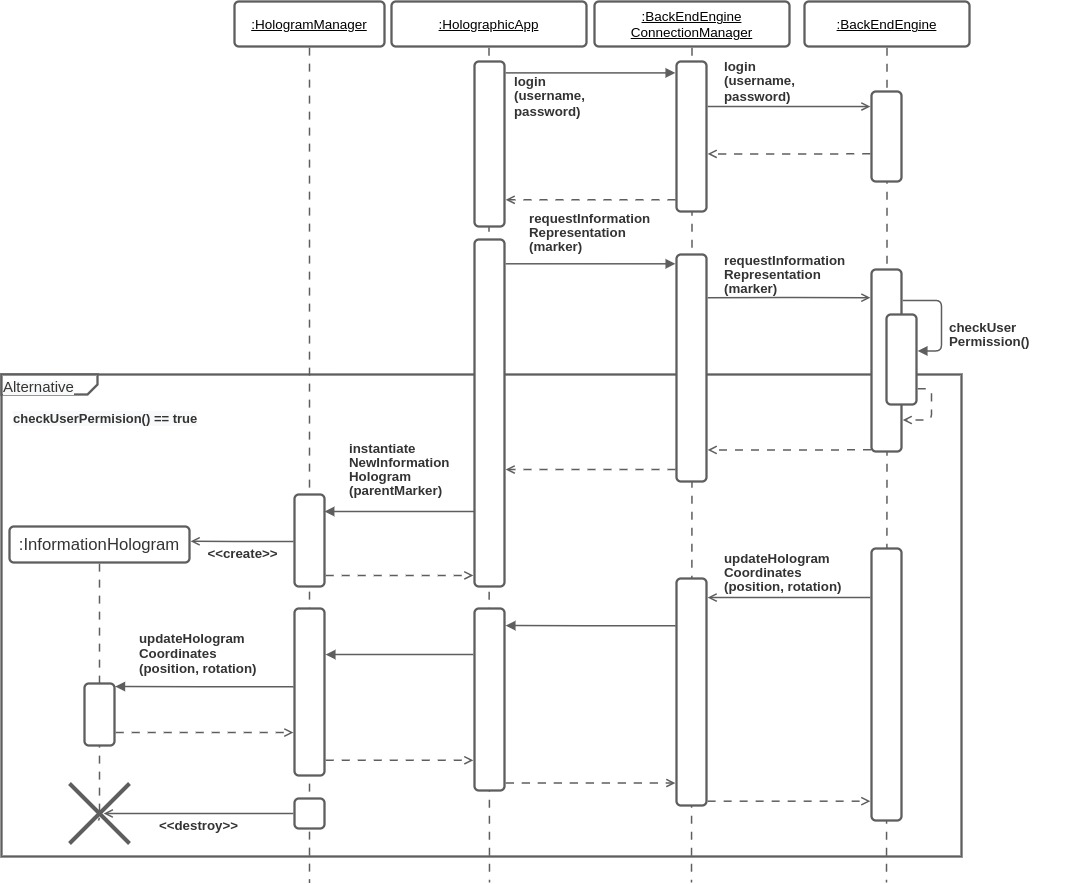
\includegraphics[width=\textwidth]{images/MR Client - Diagramma di Sequenza Esperienza Condivisa.jpg}
    \caption{Holographic App - Diagramma di sequenza di un'esperienza condivisa.}
    \label{fig:figure46}
\end{figure}

Un altro caso interessante viene presentato in Figura \ref{fig:figure47}.
Qui abbiamo un utente che richiede la rappresentazione di un dispositivo IoT (luce) al Back-End Engine.
In questo caso la parte in cui viene effettuato il login è stata omessa per alleggerire il carico grafico, ma viene comunque eseguita.
Una volta controllati i permessi di accesso, il Back-End Engine restituisce la rappresentazione del dispositivo e l'ologramma relativo viene generato.
A questo punto l'utente ha la possibilità non solo di accedere allo stato della luce, ma anche di modificarlo sfruttando la sua rappresentazione.
L'utente interagisce con l'ologramma e accende la luce (che inizialmente era spenta); il \texttt{ServiceConnectionManager} invia la richiesta al Back-End Engine, che controlla ancora una volta i permessi e infine accende effettivamente la luce contattando il dispositivo IoT associato.

\begin{figure}[H]
    \centering
    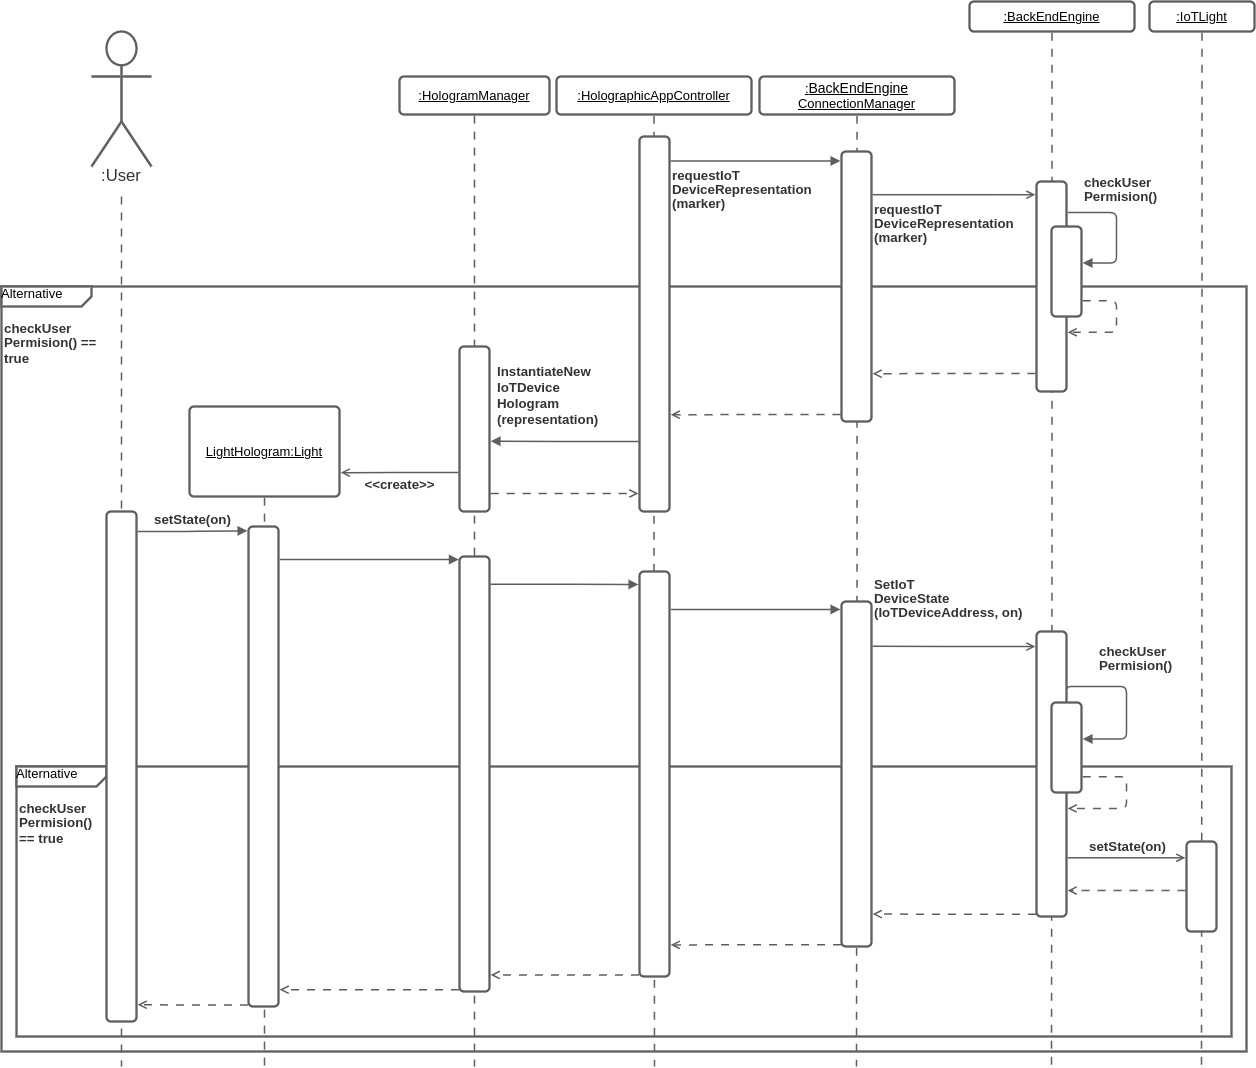
\includegraphics[width=\textwidth]{images/MR Client - Diagramma di Sequenza Dispositivo IoT.jpg}
    \caption{Holographic App - Diagramma di sequenza con un dispositivo IoT.}
    \label{fig:figure47}
\end{figure}

\section{Sviluppo del Prototipo}
\subsection{Tecnologie Utilizzate}
Per lo sviluppo del prototipo relativo al caso di studio\footnote{Repository GitHub: \href{https://github.com/FilippoVissani/three-year-degree-thesis}{https://github.com/FilippoVissani/three-year-degree-thesis}} sono state utilizzate le seguenti tecnologie:

Unity 2020 LTS è stato utilizzato come ambiente di sviluppo principale. Si è scelto di utilizzare questa specifica versione perché al momento viene considerata come miglior soluzione secondo Microsoft.

Per lo sviluppo degli script C\# presenti nell'applicazione è stato utilizzato Visual Studio 2019.

Il plugin per la gestione della realtà mista che si è scelto di integrare in Unity è OpenXR, perché nonostante sia ancora in fase sperimentale, in futuro rimpiazzerà tutti gli altri plugin esistenti.
Inoltre, OpenXR fornisce delle API comuni per tutte le principali piattaforme, una caratteristica utile se in futuro si volessero integrare dispositivi diversi da HoloLens.

Insieme a OpenXR sono stati importati i componenti del Mixed Reality Toolkit Foundation 2.7, che permettono di accedere direttamente alle funzionalità offerte da HoloLens grazie a dei profili.
Una volta aggiunto il componente a Unity, compare un menu dove è possibile aggiungere gli oggetti \texttt{MixedRealityToolkit} e \texttt{MixedRealityPlayspace} alla scena.
Tramite l'oggetto \texttt{MixedRealityToolkit} è possibile gestire i profili relativi alle funzionalità di HoloLens.

Per permettere ad HoloLens di rilevare i marker è stato utilizzato Vuforia 10.0.1 integrato in Unity.
Vuforia permette di riconoscere vari tipi di marker, basati su immagini o su modelli 3D. È possibile associare uno o più oggetti 3D o 2D al marker, nel momento in cui il marker viene rilevato gli oggetti associati vengono aggiunti alla scena.
Un aspetto importante da considerare è che i marker Vuforia non possono trasmettere informazioni come ad esempio fanno i codici QR.

Per associare un oggetto a un marker è sufficiente impostarlo come figlio nel progetto Unity.
Uno dei problemi sorti durante i test è che gli ologrammi relativi a un marker su HoloLens hanno problemi di stabilità, come sfarfallio o posizione non precisa.
Nel momento in cui l'utente si muove nell'ambiente, gli ologrammi associati a un marker possono spostarsi, assumendo una posizione con un errore considerevole. Per questo motivo bisogna trovare una soluzione che permetta di creare gli ologrammi, ma senza associare direttamente gli oggetti 3D al marker.

\subsection{Struttura del Progetto Unity}
Nella scena principale del progetto (Figura \ref{fig:figure48}) sono presenti tre componenti principali:
\begin{itemize}
    \item \textbf{MixedRealityToolkit}: utilizzato per gestire i profili relativi alle funzionalità offerte da HoloLens.
    \item \textbf{HolographicAppController}: oggetto che si occupa di inizializzare la scena a runtime, generando i marker associati alle immagini.
    \item \textbf{HologramManager}: oggetto che si occupa della gestione degli ologrammi associati ai marker.
\end{itemize}

Gli oggetti relativi ai marker e agli ologrammi non sono presenti all'interno della scena di Unity, perché questi vengono istanziati a runtime.

Per quanto riguarda i profili del MRTK sono state abilitate le seguenti funzionalità: Camera, Input, Boundary, Spatial Awareness con occlusione della mesh.

I prefab che vengono istanziati a runtime sono composti da oggetti 3D, finestre e menu.
I menu vengono utilizzati per attivare o disattivare determinate funzioni dell'ologramma. Una di queste funzioni è la capacità di seguire l'utente nell'ambiente.
Gli oggetti 3D hanno integrati i seguenti componenti:
Box Collider (utilizzato per rilevare correttamente qualsiasi tipo di collisione), Rigid Body (utilizzato per non far oltrepassare la mesh all'ologramma), Object Manipulator(utilizzato per abilitare le interazioni sfruttando il gaze), Near Interaction Grabbable (utilizzato per abilitare le interazioni da vicino), Follow Me Toggle (utilizzato per permettere all'utente di essere seguito dall'ologramma nel momento in cui si muove).

\begin{figure}[H]
    \centering
    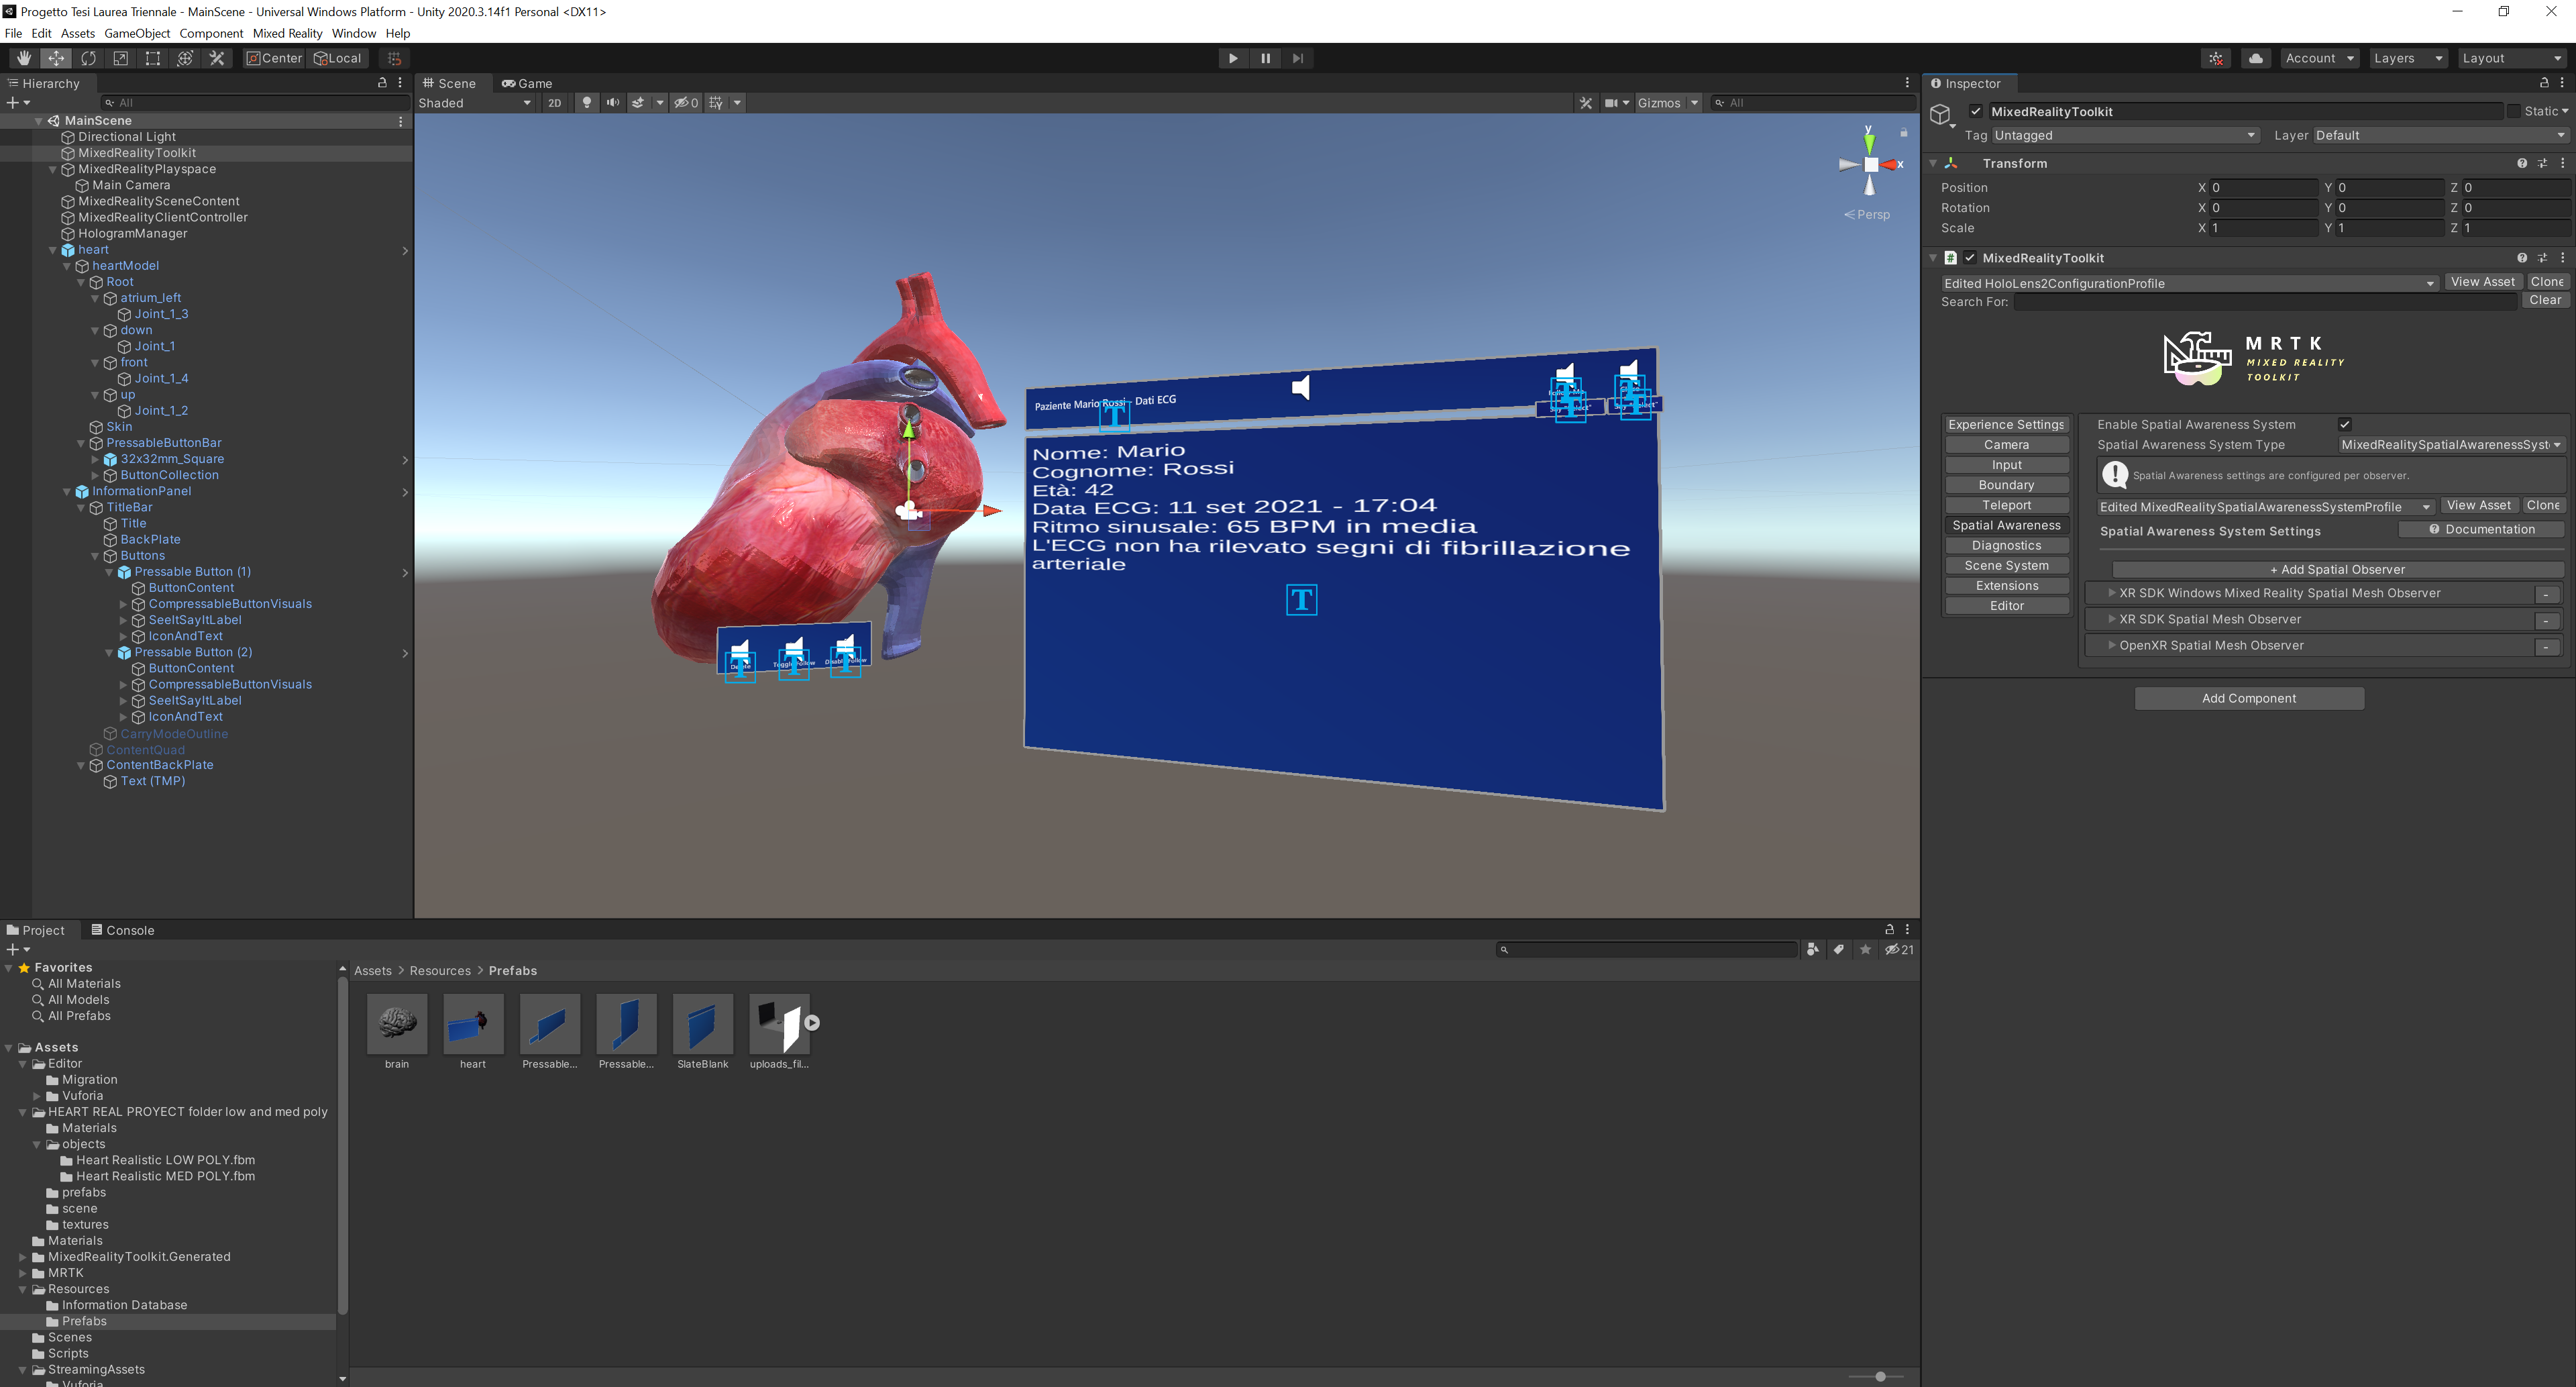
\includegraphics[width=\textwidth]{images/scena-unity-prototipo.png}
    \caption{Scena di Unity relativa al prototipo.}
    \label{fig:figure48}
\end{figure}

\subsection{Identificazione delle Informazioni nell'Ambiente}
Per identificare correttamente le informazioni sono stati utilizzati i marker Vuforia.
Ad ogni informazione è stato associato un marker, in questo modo ogni informazione può essere identificata in modo univoco.

I marker non sono stati caricati staticamente all'interno del progetto, questi infatti vengono scaricati a runtime da un servizio web presente all'interno della rete locale.

Il servizio contiene le immagini dei marker e un file Json dove le immagini vengono associate all'ologramma da istanziare.

All'avvio, l'applicazione si collega al servizio e scarica il file Json e le immagini dei marker (Listato \ref{lst:listato1}).

Per il download dei dati vengono utilizzate due coroutine\footnote{Una coroutine è come una funzione che ha la capacità di mettere in pausa l'esecuzione e restituire il controllo a Unity, ma poi continuare da dove era stata interrotta nel frame successivo.}, \texttt{GetInformationDatabase} viene richiamata per scaricare il file Json, che viene deserializzato e convertito in un oggetto di tipo \texttt{Dictionary<string, string>}. il nome del marker viene utilizzato come chiave e il nome del prefab come valore associato.

Una volta scaricato correttamente il file Json viene avviata la coroutine \texttt{DownloadMarkerImages} per scaricare le immagini dei marker.
In questa coroutine vengono considerati solo i marker presenti nel file Json. Quindi se un'immagine non viene considerata nel file Json, questa non viene neanche scaricata dall'applicazione.
Per associare correttamente l'immagine scaricata al marker viene utilizzato un oggetto di tipo \texttt{Dictionary<string, Texture2D>}.

\lstset{language=[Sharp]C, numbers=left}
\begin{lstlisting}[caption={coroutine utilizzate per scaricare il file Json e le immagini dei marker dal servizio.}, label=lst:listato1]

    IEnumerator GetInformationDatabase()
    {
        using (UnityWebRequest uwr = UnityWebRequest.Get(serverAddress + "information-database.json"))
        {
            yield return uwr.SendWebRequest();
            if (uwr.result == UnityWebRequest.Result.Success)
            {
                informationDatabase = JsonConvert.DeserializeObject<Dictionary<string, string>>(uwr.downloadHandler.text);
                StartCoroutine(DownloadMarkerImages());
            }
        }
    }

    private IEnumerator DownloadMarkerImages()
    {
        markerImages = new Dictionary<string, Texture2D>();
        foreach (var marker in informationDatabase.Keys)
        {
            using (UnityWebRequest uwr = UnityWebRequestTexture.GetTexture(serverAddress + marker + ".jpg"))
            {
                yield return uwr.SendWebRequest();
                if (uwr.result == UnityWebRequest.Result.Success)
                {
                    var texture = DownloadHandlerTexture.GetContent(uwr);
                    markerImages.Add(marker, texture);
                }
            }
        }
        currentState = State.InformationReady;
    }
\end{lstlisting}

A questo punto le immagini vengono sfruttate per creare effettivamente i GameObject relativi ai marker presenti nella scena di Unity (Listato \ref{lst:listato2}).
Questa funzionalità viene implementata sfruttando le API di Vuforia, che permettono di istanziare gli oggetti relativi ai marker a runtime.

\lstset{language=[Sharp]C, numbers=left}
\begin{lstlisting}[caption={Metodo richiamato per creare i target in base alle immagini scaricate precedentemente.}, label=lst:listato2]
    private void CreateImageTargetFromTexture(string markerName, Texture2D image)
    {
        var mTarget = VuforiaBehaviour.Instance.ObserverFactory
        .CreateImageTarget(image, 0.1f, markerName);
        mTarget.gameObject
        .AddComponent<DefaultObserverEventHandler>();
    }
\end{lstlisting}

\subsection{Gestione degli Ologrammi Relativi alle Informazioni}
La gestione degli ologrammi dell'applicazione viene delegata allo script \texttt{HologramManager.cs}.
Questo script si occupa di associare a ogni marker un pulsante, che genera l'ologramma associato una volta premuto (Listato \ref{lst:listato3}).
Ci sono vari motivi per cui, nel momento in cui si rileva un marker, si genera un pulsante e non direttamente l'ologramma associato.
L'operatore potrebbe non avere bisogno dell'ologramma anche se sta guardando il marker. Prendiamo come esempio il caso in cui si sta leggendo un documento che contiene anche il marker. Se l'ologramma venisse generato all'istante creerebbe confusione, si vuole fare in modo di crearlo solamente nel momento in cui risulta necessario all'operatore.
Un altro caso potenzialmente critico si genera nel momento in cui si osservano contemporaneamente più marker. In questo caso, evitando di usare un pulsante per ogni marker, verrebbero generati contemporaneamente tutti gli ologrammi associati, i quali occuperebbero inutilmente uno spazio nell'ambiente, creando confusione all'operatore.

A ogni pulsante viene anche associato un \texttt{Listener}, che viene richiamato alla pressione.

\lstset{language=[Sharp]C, numbers=left}
\begin{lstlisting}[caption={Metodo richiamato per associare un bottone ad ogni marker.}, label=lst:listato3]
    public void addHologram(string marker, string hologram)
    {
        GameObject buttonInstance = Instantiate(buttonPrefab);
        buttonInstance.transform.eulerAngles = new Vector3(90f, 0f, 0f);
        buttonInstance.transform.parent = GameObject.Find(marker).transform;
        buttonInstance.GetComponent<Interactable>()
        .OnClick.AddListener(() => SpawnHologram(marker, hologram));
    }
\end{lstlisting}

Il metodo \texttt{SpawnHologram} (Listato \ref{lst:listato4}) viene associato a ogni pulsante, alla pressione del quale viene istanziato il prefab associato.

\lstset{language=[Sharp]C, numbers=left}
\begin{lstlisting}[caption={Listener richiamato per generare l'ologramma associato al marker.}, label=lst:listato4]
    private void SpawnHologram(string marker, string hologram)
    {
        GameObject hologramInstance = Instantiate(Resources.Load<GameObject>("Prefabs/" + hologram));
        hologramInstance.transform.position = new Vector3(GameObject.Find(marker).transform.position.x,
            GameObject.Find(marker).transform.position.y + 0.2f,
            GameObject.Find(marker).transform.position.z);
    }
\end{lstlisting}

\subsection{Allineamento dei Sistemi di Coordinate}
L'allineamento dei sistemi di coordinate fra più dispositivi è necessario nel momento in cui si partecipa a un'esperienza condivisa.
Per realizzare questa funzionalità si può procedere sfruttando:
\begin{itemize}
    \item Azure Spatial Anchors
    \item Sistema di condivisione delle posizioni degli ologrammi realizzato su misura.
\end{itemize}

Azure Spatial Anchors permette di condividere in allineamento spaziale e temporale le ancore presenti in un ambiente. Tuttavia, non è possibile interagire direttamente con un ologramma ancorato, per permettere l'interazione bisogna prima eliminare l'ancora.
Questo significa che più utenti non possono interagire contemporaneamente con lo stesso ologramma, perché non c'è modi di condividere la fase di interazione.
Per questo motivo è opportuno realizzare un sistema più adeguato al caso di studio, che permetta di condividere anche le interazioni degli utenti con gli ologrammi.

Nelle applicazioni HoloLens realizzate con Unity l'origine del mondo viene impostata in corrispondenza del punto in cui si è avviata l'applicazione.
Questo è un problema per la realizzazione delle esperienze condivise, perché diversi dispositivi hanno sistemi di coordinate con origine in punti differenti, quindi non è possibile condividere direttamente la posizione degli ologrammi.
Un modo per realizzare questa funzionalità è sfruttare il sistema di coordinate esposto dai marker Vuforia e il Back-End Engine, che permette la condivisione delle coordinate degli ologrammi fra più client.

Nel momento in cui un client interagisce con un ologramma la nuova posizione viene inviata al servizio (Listato \ref{lst:listato5}).
Il servizio, nel momento in cui riceve una nuova posizione, la replica su tutti gli altri client sfruttando le WebSocket (Listato \ref{lst:listato6}).

\lstset{language=[Sharp]C, numbers=left}
\begin{lstlisting}[caption={Il client manda la nuova posizione dell'ologramma la servizio.}, label=lst:listato5]
    private async void SendPosition()
    {
        Vector3 position = childGameObject.transform.position - marker.transform.position;
        string message = "{\"X\":" + position.x
                        + ", \"Y\":" + position.y
                        + ", \"Z\":" + position.z + "}";
        await ws.SendText(message);
        lastPosition = childGameObject.transform.position;
    }
\end{lstlisting}

\lstset{language=[Sharp]C, numbers=left}
\begin{lstlisting}[caption={Il servizio replica la nuova posizione ricevuta su tutti gli altri client.}, label=lst:listato6]
wss.on('connection', function connection(ws, req) {
    ws.on('message', function incoming(data) {
        wss.clients.forEach(function each(client) {
        if (client !== ws && client.readyState === WebSocket.OPEN) {
            client.send(data);
        }
    });
  });
});
\end{lstlisting}

\subsection{Persistenza degli Ologrammi nel Tempo e nello Spazio}
In determinati casi può essere necessario ancorare gli ologrammi all'ambiente in modo persistente.

Prendiamo ad esempio il caso un cui un ambiente sia stato arredato con entità virtuali, magari anche in condivisione con più utenti.
Può essere utile memorizzare posizione e rotazione degli ologrammi in modo persistente, perché altrimenti questi ultimi andrebbero riposizionati manualmente a ogni avvio dell'applicazione.

Per far persistere un ologramma localmente in un dispositivo è possibile utilizzare i sistemi di ancore offerti dal MRTK.
Per le diverse versioni di Unity presenti oggi sono disponibili diversi sistemi di gestione delle ancore.
Le API messe a disposizione permettono di salvare in modo persistente la posizione di un ologramma in un determinato ambiente.
Attraverso diverse sessioni HoloLens riconosce l'ambiente e mette a disposizione le ancore salvate nelle sessioni precedenti.
Tuttavia, questa funzionalità ha delle forti limitazioni, perché è possibile memorizzare le ancore solo localmente.
Una possibile soluzione sarebbe utilizzare i servizi Azure, che permettono di condividere le ancore in cloud.
L'unico problema è che al momento i servizi di condivisione delle ancore offerti da Azure sono compatibili solo con HoloLens e altri prodotti Microsoft. Quindi, per permettere di integrare dispositivi differenti, si è scelto ancora una volta di utilizzare il Back-End Engine.

Sfruttando il Back-End Engine è possibile far persistere un ologramma nello spazio e nel tempo, in altre parole è come realizzare un sistema di ancore simile al servizio offerto da Azure.
L'utilizzo del servizio consente all'ologramma di "esistere" indipendentemente dal fatto che nell'ambiente ci siano utenti che interagiscono con esso.
All'avvio dell'applicazione viene contattato il servizio e vengono scaricati gli ologrammi con le relative posizioni.
Ogni volta che posizione o rotazione di un ologramma vengono modificate il servizio viene informato.

\subsection{Prototipo in Esecuzione}
All'interno del prototipo sono stati inseriti prefab relativi a varie informazioni, una delle quali è il risultato di un ECG di un paziente (Figura \ref{fig:figure49}). Questo documento presenta i dati del paziente in questione, il risultato dell'ECG e il marker associato al documento.

\begin{figure}[H]
    \centering
    \includegraphics[scale=0.5, frame]{images/ecg.jpg}
    \caption{Esempio di documento contenente informazioni e marker.}
    \label{fig:figure49}
\end{figure}

In fase di esecuzione, il prototipo si collega al server presente in LAN e scarica il file Json che si occupa di associare il nome del prefab al marker. Successivamente vengono scaricate anche le immagini relative marker che vengono riportati nel file Json.
In questo caso il file Json contiene una entry del genere: \texttt{"marker1":"heart"}.

A questo punto l'oggetto relativo al marker viene istanziato, così quando lo si osserva può essere rilevato correttamente.
Nel momento in cui il marker viene riconosciuto dal prototipo, viene creato un pulsante (Figura \ref{fig:figure410}) che permette di istanziare il prefab associato.
\begin{figure}[H]
    \centering
    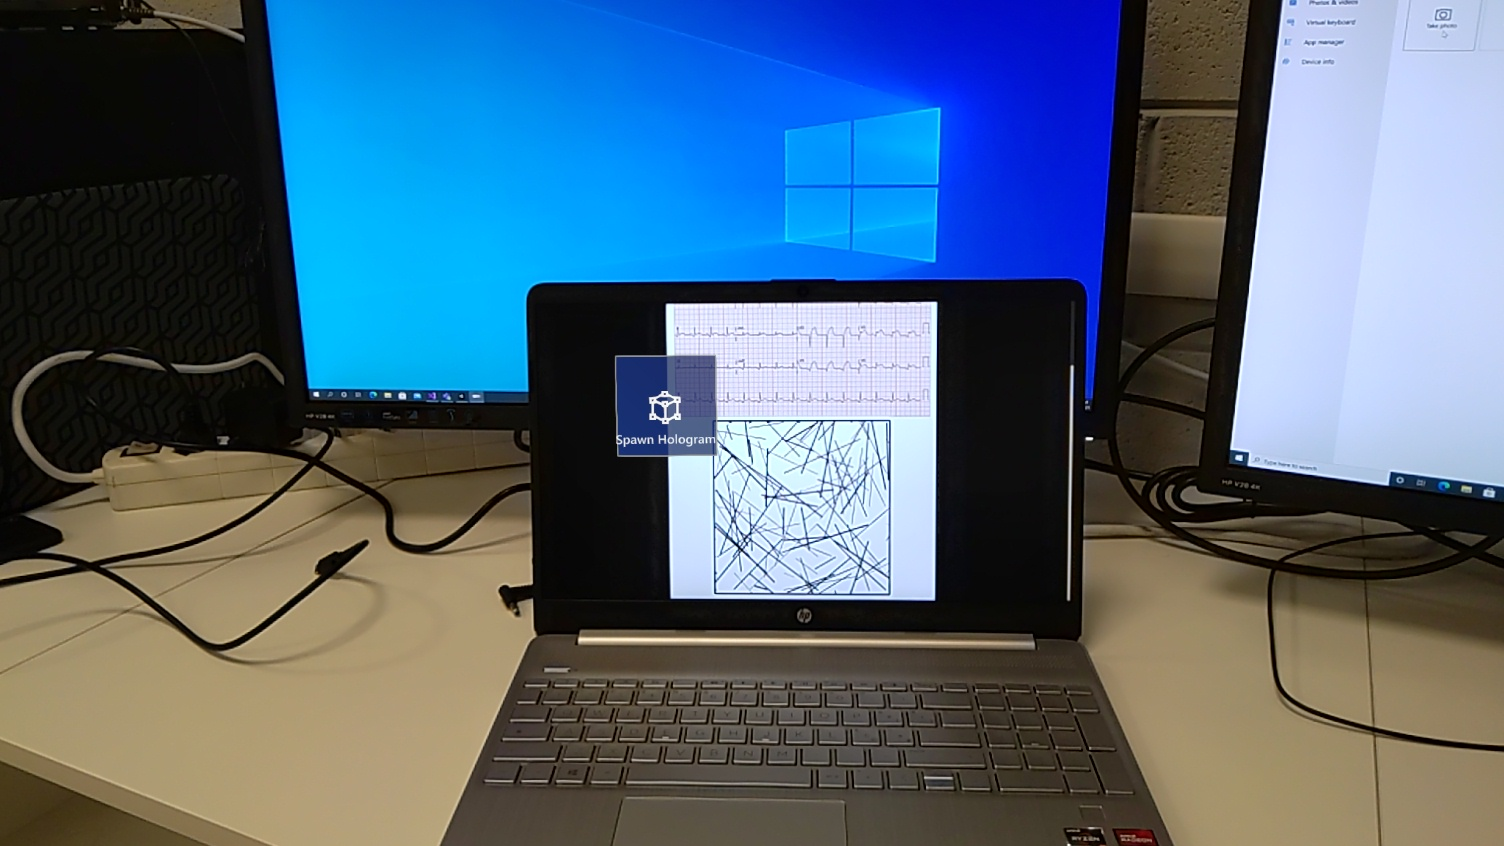
\includegraphics[width=\textwidth]{images/ecg-marker-button.jpg}
    \caption{Nel momento in cui viene inquadrato il marker viene generato un pulsante che permette di creare l'ologramma.}
    \label{fig:figure410}
\end{figure}

Una volta premuto il pulsante relativo al marker presente nel documento in Figura \ref{fig:figure49} vengono istanziati due ologrammi: il modello 3D del cuore del paziente e una finestra che riporta le stesse informazioni presenti nel documento (Figura \ref{fig:figure411}).
A questo punto l'operatore è libero di posizionare gli ologrammi all'interno dell'ambiente come preferisce.

Sia la finestra che il cuore dispongono di un menu che permette di eliminarli e di attivare la funzionalità Follow Me, la quale permette all'utente di essere seguito dall'ologramma nel momento in cui si muove.

\begin{figure}[H]
    \centering
    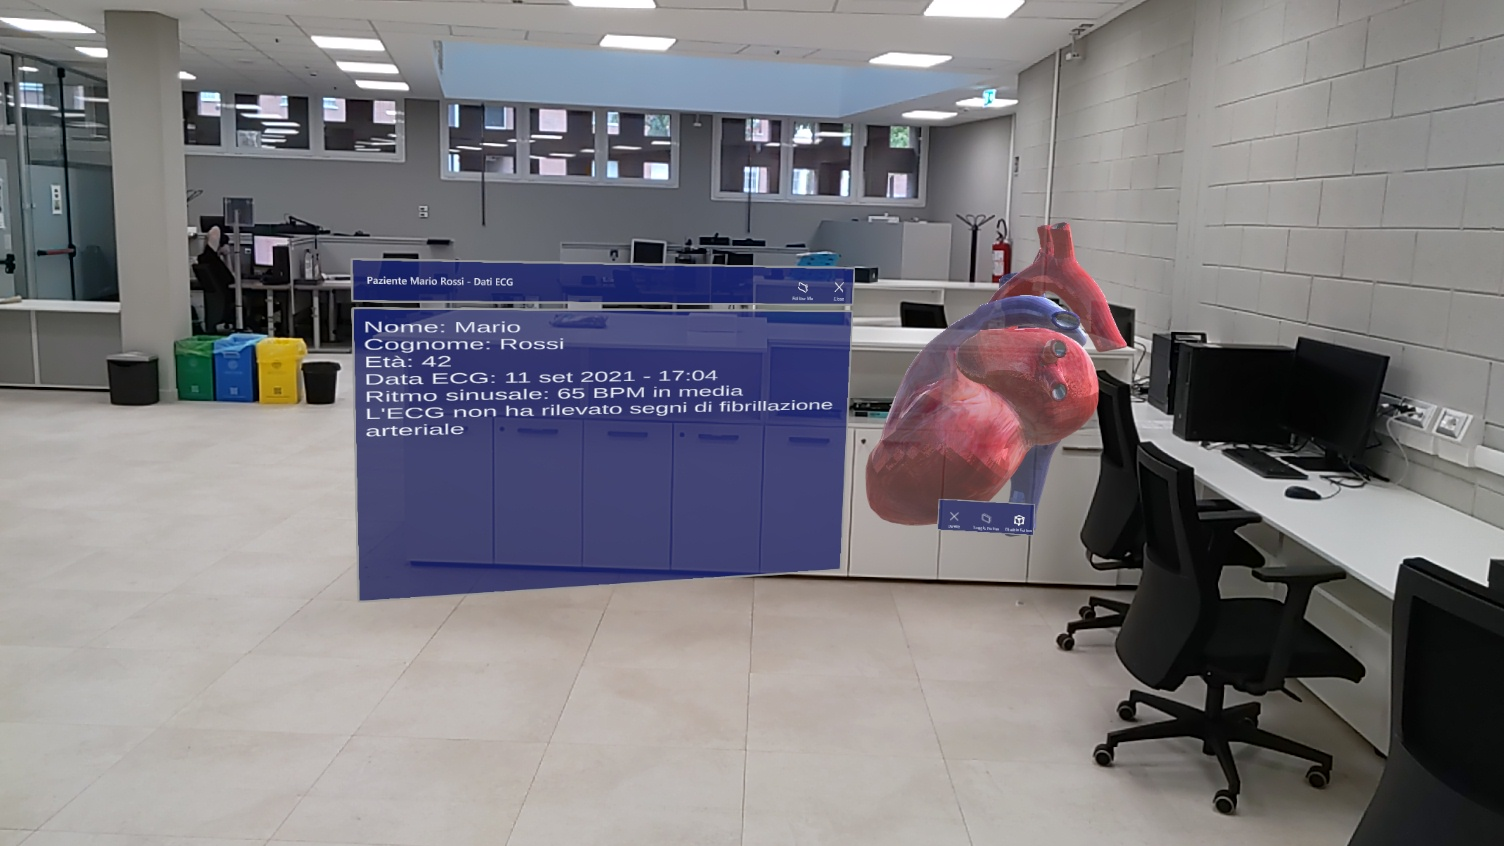
\includegraphics[width=\textwidth]{images/ecg-hologram.jpg}
    \caption{Ologrammi relativi al documento in Figura \ref{fig:figure49}.}
    \label{fig:figure411}
\end{figure}

\section{Considerazioni Finali}\label{sec:sezione45}
Con questo caso di studio si è dimostrata l'utilità della realtà mista in ambito sanitario, ma il sistema proposto può essere riutilizzato in tutto o in parte anche in altri ambiti.
Il sistema può inoltre essere esteso, ampliando i casi in cui può essere utilizzato. Alcune delle possibili integrazioni che possono essere fatte vengono presentate nella sottosezione successiva.

Per quanto riguarda lo sviluppo del prototipo con MRTK e Unity è bene fare una precisazione: alcune delle funzionalità del MRTK sono ancora in fase sperimentale e Unity è stato progettato per sviluppare videogiochi, non applicazioni Mixed Reality.
A causa di questi aspetti, creare e configurare correttamente un progetto per HoloLens 2 è un'operazione estremamente complessa e che richiede molto tempo.
Avere un ambiente di sviluppo progettato appositamente per creare applicazioni Mixed Reality risolverebbe questo problema.

\subsection{Sviluppi Futuri}
Il macrosistema presentato nella sezione \ref{sec:Sezione4.3} è stato concepito per essere esteso, in modo da poter aggiungere ulteriori servizi e integrare nuovi dispositivi.
Applicando determinate modifiche può anche essere riutilizzato in altri ambiti, oltre a quello sanitario.
Sviluppando applicazioni specifiche per ogni piattaforma, è possibile coinvolgere nelle esperienze di realtà mista dispositivi differenti, come smartphone o smart-glasses.

Invece per quanto riguarda le rappresentazioni, queste potrebbero essere generate dinamicamente.
Prendiamo come esempio un display che riporta grafici dinamici, come l'andamento del battito cardiaco di un paziente.
Può essere utile avere una rappresentazione sotto forma di ologramma di ciò che il display sta mostrando.
Sfruttando al massimo la potenza della realtà mista, determinati strumenti potrebbero anche essere sostituiti completamente dalle loro rappresentazioni.

Si potrebbe anche gestire una rappresentazione degli operatori, in modo da permettere esperienze condivise sfruttando la telepresenza. In questo tipo di esperienza gli operatori possono collaborare pur non trovandosi fisicamente nello stesso ambiente.
La telepresenza consentirebbe all'operatore di sentirsi come se fosse presente in un luogo diverso dalla sua vera posizione.
Gli operatori presenti nell'ambiente avrebbero la possibilità di interagire con quelli in telepresenza grazie alle rappresentazioni digitali di questi ultimi.

\chapter*{Conclusioni}
\addcontentsline{toc}{chapter}{Conclusioni}
\markboth{CONCLUSIONI}{CONCLUSIONI}
Traendo le conclusioni, in questa tesi sono stati presentati i risultati degli studi effettuati a proposito dello sviluppo di applicazioni Mixed Reality per HoloLens 2.

Il campo della realtà mista è molto ampio, può essere descritto secondo svariati punti di vista e avere infinite applicazioni.
La definizione stessa di realtà mista si perfeziona con l'introduzione di nuove tecnologie che realizzano quest'ultima.

Nei quattro capitoli di questa tesi viene più volte evidenziato il fatto che HoloLens 2 è un dispositivo unico nel suo genere, che introduce importanti novità tecniche.
Nessun altro dispositivo in commercio è in grado di rilevare l'ambiente e di proiettare ologrammi permettendo all'utente di interagirci come se fossero reali, nel modo in cui lo fa HoloLens 2.
La realtà mista, della quale fino a qualche anno fa si è solo parlato da un punto di vista teorico, ora può essere concretizzata grazie ad HoloLens 2.

Tuttavia, questa tecnologia ha ancora dei limiti, come gli strumenti di sviluppo, che sono in parte ancora in fase sperimentale.
Come detto nella Sezione \ref{sec:sezione45}, un ambiente di sviluppo creato su misura risolverebbe i problemi che si sono presentati durante le fasi di studio e di sviluppo.
Probabilmente nei prossimi anni verrà fornito un supporto migliore per lo sviluppo di queste applicazioni.

Bisogna anche considerare che al momento gli utenti che hanno la possibilità di utilizzare HoloLens non sono molti perché inizialmente è stato commercializzato solo negli Stati Uniti, per poi essere reso disponibile in altri paesi solo nel corso del 2020.
Probabilmente in futuro dispositivi come HoloLens verranno commercializzati su larga scala, raggiungendo un gran numero di utenti.

Alcune delle esperienze che la realtà mista permette in teoria non possono ancora essere realizzate concretamente, la telepresenza è un esempio.
Con il progresso tecnologico, le potenzialità dei dispositivi Mixed Reality verranno incrementate notevolmente, questo permetterà di realizzare tutte le esperienze che finora sono state presentate solo a livello teorico.
In futuro sarà possibile realizzare sistemi che ridurranno sempre di più il divario fra mondo reale e virtuale, fino a farlo scomparire del tutto.	
\chapter*{Ringraziamenti}
\addcontentsline{toc}{chapter}{Ringraziamenti}
\markboth{RINGRAZIAMENTI}{RINGRAZIAMENTI}

Prima di tutto desidero ringraziare il professor Angelo Croatti e il professor Alessandro Ricci, che mi hanno seguito costantemente durante il tirocinio e nella fase di stesura della tesi.

Un'altra persona che voglio ringraziare è Anna Vitali, con la quale ho sviluppato applicazioni Mixed Reality per comprendere il funzionamento di HoloLens 2 e Unity.

Ringrazio i miei genitori che mi hanno sempre sostenuto, appoggiando ogni mia decisione, fin dalla scelta del mio percorso di studi.

Infine un ringraziamento speciale va sia agli amici di una vita, che a quelli che ho conosciuto in questi tre anni di università.
	
\backmatter	

\bibliography{bibliografia}{}
\bibliographystyle{plain}

\end{document}